%%% File encoding: UTF-8
%%% äöüÄÖÜß  <-- no German umlauts here? Use an UTF-8 compatible editor!

%%% Magic comments for setting the correct parameters in compatible IDEs
% !TeX encoding = utf8
% !TeX program = pdflatex 
% !TeX spellcheck = de_DE
% !BIB program = biber

\documentclass[master,english,smartquotes,apa]{hgbthesis}
% Valid options in [..]: 
%    Type of work: 'diploma', 'master' (default), 'bachelor', 'internship' 
%    Main language: 'german' (default), 'english'
%    Turn on smart quote handling: 'smartquotes'
%    APA bibliography style: 'apa'
%%%-----------------------------------------------------------------------------

\RequirePackage[utf8]{inputenc} % Remove when using lualatex or xelatex!

\graphicspath{{images/}}  % Location of images and graphics
\logofile{logo}           % Logo file: images/logo.pdf (no logo: \logofile{})
\bibliography{references} % Biblatex bibliography file (references.bib)

% \usepackage[table]{xcolor}
\usepackage{longtable}

%%%-----------------------------------------------------------------------------
% Title page entries
%%%-----------------------------------------------------------------------------

\title{ Application of Software Quality Measures to Bare-metal Firmware for Optical Coherence Tomography}
\author{Florian Hinterleitner}
\programname{embedded systems design}
\programtype{Fachhochschul-Masterstudiengang}
\placeofstudy{Hagenberg}
\dateofsubmission{2022}{06}{15} % {YYYY}{MM}{DD}
\advisor{Langer, Rankl, Zorin} % optional
%\strictlicense % restrictive license instead of Creative Commons (discouraged!)
\definecolor{gray}{gray}{.80}

\newcommand{\GREY}[1]{\textcolor{gray}{#1}}
\newcommand{\TODO}[1]{\textcolor{red}{\textbf{ToDo:} #1}}
\newcommand{\RED}[1]{\textcolor{red}{#1}}
\newcommand{\redrow}[1]{{#1}}
\newcommand{\BLACK}[1]{\textcolor{black}{#1}}
\newcommand{\BLUE}[1]{\textcolor{blue}{#1}}
\newcommand \bild[4]{\begin{figure}[#1]	\centering	\includegraphics[width=\textwidth]{images/#2}	\caption{#3}	\label{#4}	\end{figure}}
\newcommand \bildGr[5]{\begin{figure}[#1]	\centering	\includegraphics[width=#5]{images/#2}	\caption{#3}	\label{#4}	\end{figure}}
% \newcommand{\redrow}{\rowcolor{red!70}}

\newcommand{\req}[9]
{
		\begin{table}[H]
		\begin{tabular}{|p{3cm}|p{12cm}|}
		% \hline
		\hline 	Tag #1		& \begin{tabular}{p{7.5cm}|l|l} #2 & Module & #9 \end{tabular} \\
			% \hline Priority				& \begin{tabular}{p{7.5cm}|l|l} #3 & Status & #4 \end{tabular}  \\		% (h)igh/(m)id/(l)ow
			\hline Description				& #5 \\															% todo/WIP/test/done
			% \hline Input				& \begin{tabular}{p{7.5cm}|l|l} #6 & Output & #8 \end{tabular} \\
			% \hline Operation			& #7 \\
			\hline
		\end{tabular}
		\label{#1}
	\end{table}
}


\lstdefinestyle{Codeschnipsel}{
language=C,
basicstyle=\sffamily\small,
keywordstyle={\color{blue}\bfseries},
%identifierstyle={\color{DarkRed}},
commentstyle={\color{green}\slshape},
stringstyle={\color{orange}},
backgroundcolor={\color{Cornsilk}},
%columns=fullflexible,
frame=shadowbox,
rulesepcolor=\color{green},
morekeywords={uint8_t, uint16_t, uint32_t, bool}, % eigene Keywörter
basewidth={0.4em,0.3em},
fontadjust=true,
breaklines=true,
showspaces=false,
showtabs=false
}


\newcommand{\lstC}{\lstinline[style=Codeschnipsel]}



\begin{document}
\frontmatter                                   % Front part (roman page numbers)
\maketitle

\tableofcontents

% \chapter{Preface}

This document uses the APA citation and reference style (see Ch.\ \ref{cha:Literature} for details).




 % A preface is optional
% \chapter{Abstract}


This should be a 1-page (maximum) summary of your work in English.

		
% \chapter{Kurzfassung}

\begin{german}
Die Firma RECENDT GmbH entwickelt und baut OCT-Systeme (optical coherence tomography), f{\"u}r die im Rahmen dieser Diplomarbeit ein Teil der Steuerung entworfen werden soll. Zur 2-dimensionalen Messung mit OCT-Systemen kommen Galvanometer-Scanner im X/Y-Betrieb zum Einsatz. Das sind hochdynamische Drehantriebe f{\"U}r optische Anwendungen, die mit einer Rate von rund 500Hz etwa 20\textdegree vor- und r{\"u}ckw{\"a}rts rotieren k{\"o}nnen. Sie tragen mitrotierende Spiegel um den optischen Pfad in 2 Dimensionen auszulenken und somit fl{\"a}chige Scans zu erm{\"o}glichen. \\

Die ausgew{\"a}hlten Galvo-Modelle ben{\"o}tigen Steuersignale zur Erzeugung der Scan-Muster. Typischerweise sind dies zwei synchrone Rampen-Signale, eines schnell, eines langsam. Aufgabe ist es nun, auf bestehender Mikrocontroller-Hardware einen Signalgenerator zu programmieren. Dieser soll sowohl Rampen-Signale als auch arbitr{\"a}r gew{\"a}hlte Signalformen erzeugen k{\"o}nnen. Dies beinhaltet FW-Module f{\"u}r die Digital-Analog-Wandler, Trigger-Einheit f{\"u}r das Timing sowie Synchronisation der Kan{\"a}le. Weiters ist die USB-Kommunikation per SCPI-Protokoll zu programmieren. Die Anbindung an eine {\"u}bergeordnete Steuerung des OCT-Systems erfolgt per USB. Die handels{\"u}blichen Galvo-Scanner besitzen mechanische Tr{\"a}gheiten, die bei Scan-Raten ab 800Hz kein maximale Auslenkung mehr erlauben. Deshalb w{\"u}rde bei hohen Geschwindgkeiten der optische Messbereich eingeschr{\"a}nkt werden. Um auch bei h{\"o}heren Scan-Raten volle Auslenkungen zu erreichen, soll versucht werden, mit adaptierten Steuersignalen die Tr{\"a}gheiten auszugleichen. \\
\end{german}			
\mainmatter                                    % Main part (arabic page numbers)
\chapter{Introduction}
\label{cha:Introduction}


\section{Motivation}
The RECENDT GmbH  is an Austrian, non-university research institute specialized in non-destructive testing. It researches, develops and produces, among other technology areas, measurement systems employing optical coherence tomography. A key element of such OCT-systems are galvanometer-scanners.  These allow for investigation of areas, instead of only point-wise measurements, by manipulating a laser-beam. This manipulation again, has to be controlled via two separate steering-voltages, one for manipulation in x-, the other in y-axis. An existing microcontroller-board, providing two sufficiently precise and fast analogue outputs, is to be programmed. This will result in the 'OCTane', a signal-generator for mentioned steering-voltages, controllable via USB. The resulting firmware shall also incorporate a HAL (hardware abstraction layer), utilizing several other functionalities, the microcontroller has to offer. Optionally, adapted signals for the steering voltages shall be investigated to allow linear control over galvanometer-scanners in higher frequency ranges.

\section{Optical coherence tomography}
Optical coherence tomography (OCT) is an imaging method for the analysis of transparent and semi-transparent materials. It shows similarities to the measurement processes via ultrasound or radar. The sample to be measured is subjected to an electromagnetic wave, the resulting 'echoes' are analysed with regard to their times of flight, as well as their intensity. From these run-times,  the geometric structure is determined, including the layer structure of the sample and also the maximum penetration depth of the applied wave. This creates a single point 1D-measurement, with that one dimension being the depth direction of the sample. This electromagnetic wave is generated by a coherent broadband light source in the visible, up to the near infrared spectrum. Coherent means, that several wave-bundles of a light source must have a fixed phase relationship to each other. This is necessary to obtain stable interference patterns. For the detection of the echoes, however, conventional photodetectors or cameras do not suffice, on the one hand due to the propagation speed of light, on the other hand due to the low reflected light intensities. Therefore, interferometry is used to detect the back reflected light. In interferometry, a laser beam is split into two waves. One wave is sent on an optical reference path of known length, the other to the surface of the sample. The reflections, the returning waves are superimposed and, depending on the nature of the sample material, result in constructive or destructive interference. This interference can be detected using a photodetector, or a spectrometer and used for further processing. A single point measurement and its depth information about the material under test is called an A-scan. Aggregation of A-scans along a line (x-direction) across the sample material, forms a B-scan. Aggregation of B-scans along a line in the y-direction result in a volume scan, i.e. a spatial, three-dimensional image of the sample material. Relevant parameters of OCT systems are the penetration depth, the axial and lateral measurement range, axial and lateral resolution and the measurement speed. While the penetration depth of ultrasound typically reaches a few centimetres and a resolution in the millimetre range, OCT allows only to look a few millimetres below the surface, but with micrometer resolutions. Measurable areas, or field-of-view, in ultrasound is in the order of centimetres, with OCT in the order of millimetres. achievable speed al results from A-scan rates up to 100kHz. The term 'optical coherence tomography' results on the one hand from the coherent light source. The other two parts of the name, 'tomos' means slice or section, and 'graphein' stand for writing or drawing, and both come from Greek. They reflect that the resulting image is assembled from individual slices or sectional images. 
The manipulation of the light beam along the mentioned lines takes place with rotatably mounted mirrors, one for the x- one for the y- direction. The faster this rotation is possible, the faster OCT-images can be created. One widespread technical realization, allowing very fast rotation of the mirrors called a galvanometer-mirror or -scanner.

\section{Galvanometer-Scanners}
% \TODO{Buedln ausm WIA-Papaer holen} \\
% \TODO{'scanner' statt 'mirror'} \\
Galvanometer scanners (colloquial: galvos) are highly dynamic opto-mechanical components, based on the classic galvanometer according to Hans Christian Oersted: A rotatable, magnetizable object, e.g. a magnetic needle, that will be deflected from its position in the proximity of a current-carrying conductor. The low sensitivity of the effect on the current is improved by a high number of windings of the electric conductor around the deflectable object, creating an electrical inductance, a coil. The non-linear connection between current and deflection angle can be linearized to a first-order approximation, by placing the coil between a rigidly positioned iron-cylinder inside and a permanent-magnet, which is arranged outside the coil \cite{keithleyHistory}. 
If this classic galvanometer is equipped with a mirror as a rotatable object, optical paths, specifically: the beam-path of a point light source, can be manipulated in one space dimension. Feasible for technical applications is, that this manipulation can be controlled reasonably linear by the current or voltage at the galvo coil. With the galvanometer-scanner employed for this master-thesis, power-electronics for the conversion of control signals to the required coil-currents and -voltages were already included. Therefore, furthermore, only 'control signals' will be discussed, instead of currents and voltages. A combination of two galvanometer scanners in a suitable geometric arrangement, irradiated with a point laser, allows to manipulate this point in two dimensions. Such an arrangement is shown in fig. ~\ref{DetailGalvoOn}. At sufficient speed, at which the laser point is deflected, 2-dimensional contours can be projected, resulting in a 'stationary' image for the human eye. It shall be noted, that only closed geometric figures are possible, as long as the light source itself cannot be turned off. These components are commercially available as laser scanner and used for light effects at music events, art installations and in discotheques. Applied to OCT-systems, on the other hand, galvanometer scanners are used to expand the measurement area from a single point of interest. Scanning mentioned coherent light over an area of the examined sample, allows for three dimensional analysis of the sample. If a dedicated x- and a y-galvo are to be steered with a slow and a fast ramp, respectively, it results in a rectangular illumination of the sample, the preferred pattern for OCT-systems. This way, raster scanning can be applied to samples.

\begin{figure}[h!]	\centering	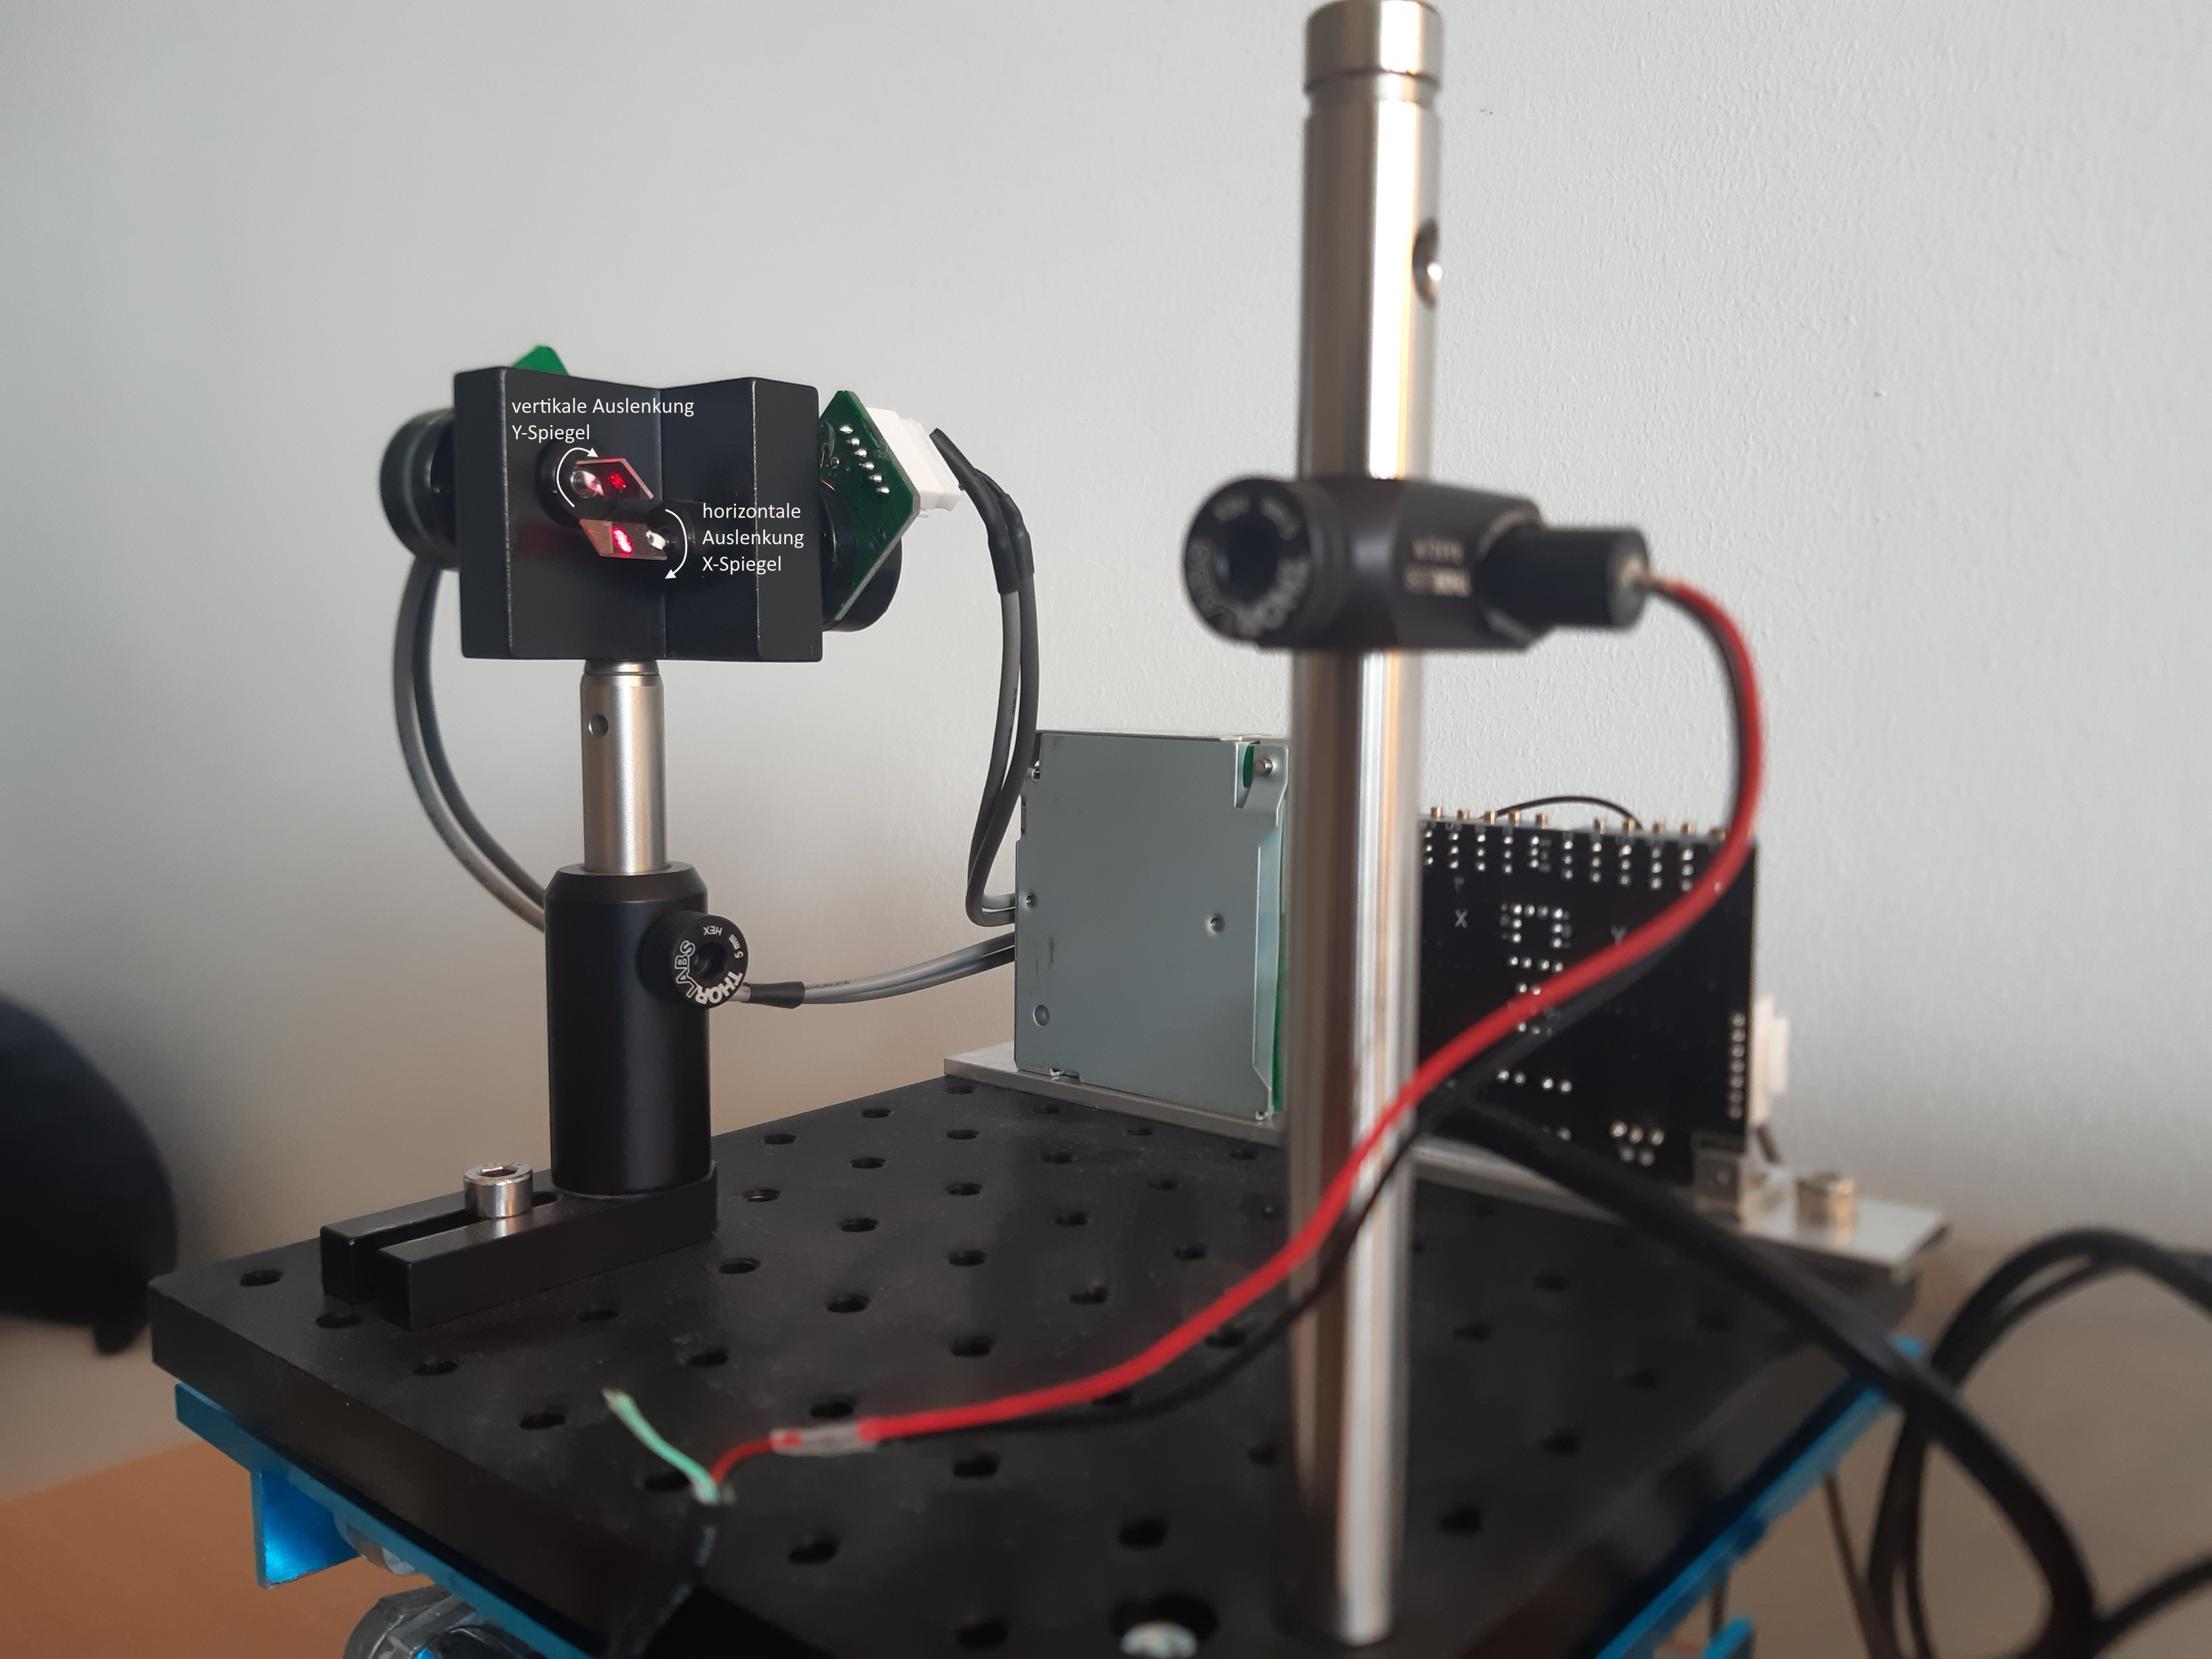
\includegraphics[width=\textwidth]{images/DetailGalvoOn.jpg}	\caption{DetailGalvoOn}	\label{DetailGalvoOn}	\end{figure}
\begin{figure}[h!]	\centering	\includegraphics[width=\textwidth]{images/DutTop02.jpg}	\caption{DutTop02}	\label{DutTop02}	\end{figure}

\section{Control of Galvanometer-Scanners}
Commercially available galvanometer scanners usually allow control in the form of analogue voltage inputs with a range of $\pm$ 10volts. The angle of the rotated mirror follows that control-voltage in a linear manner for sufficiently low frequencies. The signal-forms to result in the rectangular scan-grids, as described in the previous section, are depicted in fig.~\ref{GalvoRamps01}. To achieve these signals, a microcontroller-board was designed, including 16-bit analogue outputs, USB-connectivity and coaxial trigger outputs, among other features. To utilise these features and form an arbitrary signal generator for mentioned ramp-signals, a firmware is necessary. This should be done in a fashion employing quality-assurance during the implementation-process, as well as the verification-phase of the firmware and its supporting hardware. Aside from signal-generation and USB-connectivity, additional features are desirable, such as user-controllable relays, utilisation of watchdog-timer, UART-, I2C- and SPI-ports as well as analogue inputs. The combination of hard- and firmware will be called OCTane. Fig. ~\ref{blocktane} demonstrates the involvement of an OCTane into an OCT-system.
\bildGr{h!}{blocktane.pdf}{Integration of an OCTane}{blocktane}{0.75\textwidth}

\begin{figure}[h!]	\centering	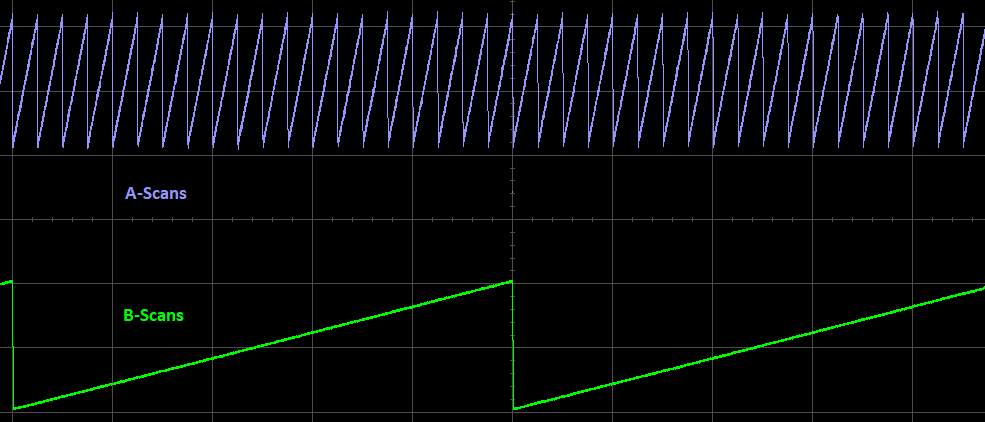
\includegraphics[width=\textwidth]{images/GalvoRamps01.png}	\caption{GalvoRamps01}	\label{GalvoRamps01}	\end{figure}
This leads to the scientific problem at hand: 
\begin{center} {\bf How can measures of quality be applied to a bare-metal firmware?}
\end{center}
% \subsection{optional: adapted steering curves}
% ...fliegt wohl raus
% \TODO{Modell ausm Paper per flachheitsbasierter Reglung auf Steuer-rampen draufrechnen}
% \textcolor{grey}{  }

\chapter{Fundamentals - Code Quality and Real-Time}
\label{cha:Fundamentals}
	\section{Motivation}
	The areas of applications for microcontrollers, as well as the complexity of their software continues to grow. Also the demands towards correct and reliable function of those systems increase accordingly. Therefore software development requires significantly more effort than development of the corresponding hardware. As the lifespan of a software surpasses that of the corresponding hardware, these efforts becomes a sensible investment. To obtain the most value from that software-product, it has to fulfil certain quality measures. Neglecting these quality aspects would lead to an unjustifiable amount of work necessary for maintenance, when the product is already in service. Examinations of the dynamics of software development indicate, that, the later in a project lifecycle, changes become necessary, the higher the expenses. The worst case scenario: errors are induced in the implementation, persist unnoticed through testing and verification. Finally, this errors appear as faults in operation at the customer site. Furthermore, if the project suffers from lazy documentation and insufficient structure, identifying these errors and correcting them becomes even more expensive. The increasing complexity of nowadays software further escalates the problem. An even worse phenomenon can arise: Insufficient understanding of a faulty piece of software can lead to introducing even more errors with additional code, that is actually intended to fix a bug. Especially when poor structuring masks hidden dependencies between modules. A general rule of thumb is: The earlier an error originates, for example in the phase of gathering requirements, the more extensive changes are necessary, later on. In other words: The earlier an error is originates and the later it emerges, the more expensive are its consequences. Pursuing a sufficient quality level from the beginning of the project, significantly reduces waste of money, hours and enthusiasm on unnecessary maintenance. It may also substantially increase the customers approval \cite{Luo2001SoftwareTT}. % \TODO{Absatz}

	The described problems have suitable solutions. Applying the appropriate methods, implemented software can become reliable, easy to change, inexpensive to maintain and allow a more intuitive understanding. Distinguishable into two categories, these methods are either analytical or constructive. \\
	
	Best practice is to apply a circular combination of constructive and analytical methods. Constructive methods alone assist in preventing errors, but do not guarantee their absence. Analytical methods are capable of demonstrating the absence of errors, but not their prevention. Therefore a large amount of preventable errors might emerge, by exclusively applying analytical methods. The combined use consists of constructive methods during every phase of a development project, and assessing the intermediate results with analytical methods by the end of each phase. This process is called the "principle of integrated quality assurance" \cite{Liggesmeyer2002}. If the intermediate results do not meet the arranged quality criteria, the current state of the project does not reach the next phase, but remains in the extended current phase. This implies, that the current state of the product requires further development, until it fulfils all necessary quality criteria. This phase- and quality driven conduct, supports the development team in detection of errors at an early point and their removal at reasonable effort. Ideally, developers detect and eliminate all errors in the by the end of the same phase, where theses errors originate. This furthermore helps in minimizing the number of errors in a product over several phases. \\
	
	The described process makes it evident, that testing only a finished product is no sufficient way of ensuring high quality. Already the first intermediate result requires examination for deviations from the quality goals. Upon detection of deviations, measures have to be taken for correction at an early stage. Also an integration of constructive and analytical quality measures significantly improves the development process. While constructive methods are most helpful during the implementation activities of a phase, the corresponding assessment benefits primarily from analytical measures. \\
	
	A further incentive in testing, especially in the formal way of well defined test-cases, originates from Boris Beizers quote from "Software Testing Techniques" \cite{Beizer90}:  
	\begin{quote}
	The act of designing tests is one of the most effective bug preventers known % 
	\end{quote}
	Additionally to the safeguarding of existing functionalities and helping in detecting errors, the thought process of formal testing methods also helps in better understanding and developing of software. \\

	The early definition of quality goals is a key factor, as it allows to achieve the intended quality. It constitutes of the specification of the desired quality features, not of defining the software requirements. This has to happen even before the phase of requirement-definition, as the requirements themself are affected by aforementioned quality goals. On the other hand, testing results against quality features is also of vital importance. \\ 
	
	The typical approach of developers is, to test a program in its early stages. This is already an informal dynamic test. Inspecting the code after implementation for structural errors is the informal equivalent of a static analysis. Application of these informal methods is very common, while formal processes of testing is much less established. Ideally, testing generates reproducible results, while following well defined procedures. \\

	While hardware quality assurance often results in quantitative results, this is usually not the case for software. But processes exist for both worlds, to ensure systematic development, as well as quality assurance. Developers of systems integrating both hardware and software have to be aware of their differences. Combining the quality measures for soft- and hardware allows to consider interactions between soft- and hardware. This prevents interactions to corrupt quality goals. Developers have to specify and verify quality properties for the complete system. It is insufficient to perform this tasks on separate modules. The correct behaviour of the whole system requires demonstration, as the test results of individual modules, usually, can not be superimposed.
	
	% \TODO{... bis hier nach Langer-Review korrigiert}
	\section{Terminology and Definitions of Terms}
	To clarify regularly used terms, here are definitions in accordance with either \cite{Kopetz1997} or \cite{Liggesmeyer2002}
	\subsubsection{Quality, Quality Requirements, Quality Features, Quality Measures}
		\begin{itemize}
		\item Quality, according to the standard 'DIN 55350 - Concepts for quality management', is defined as: The ability of a unit, or device, to fulfil defined and derived quality requirements.
		\item Quality requirements describe the aggregate of all single requirements regarding a unit or device.
		\item Quality features describe concrete properties of a unit or device, relevant for the definition and assessment of the quality. While it does not make quantitative statements, or allowed values of a property, so to say, it very well may have a hierarchical structure: One quality feature, being composed of several detailed sub-features. A differentiation into functional and non-functional features is advised. Also features may have different importance for the customer and the manufacturer. Overarching all these aspects, features may interfere with each other in an opposing manner. As a consequence, maximizing the overall level of quality, regarding every aspect, is not a feasible goal. The sensible goal is to find a trade-off between interfering features, and achieve a sufficient level of quality for all relevant aspects. Typical features, regarding software development include: Safety, security, reliability, dependability, availability, robustness, efficiency regarding memory and runtime, adaptability portability, and testability.
		\item {Quality measures} define the quantitative aspects of a quality feature. These are measures, that allow conclusions to be drawn about the characteristics of certain quality features. For example, the MTTF (mean time to failure), is a widespread measure for reliability.
		\end{itemize}
	
	\bildGr{b!}{ErrorFaultFailure.pdf}{Causal chain of failures.}{ErrorFaultFailure}{0.5\textwidth}

	\subsubsection{Error, Failure, Fault}
	\begin{minipage}{\linewidth}
	\begin{itemize}
		\item {Error}, the root cause of a device or unit to fail, may originate from operation outside the specification, or from human mistakes in the design.
		\item {Failure}, or defect is the incorrect internal state of a unit, and is the result of an error. It exists either on the hard- or software-side and is the cause of a fault, but not necessarily.
		\item {Fault} is the incorrect behaviour of the unit, or it's complete cease of service, observable by the user. It is caused by a failure.
		\item These definitions are in accordance with \cite{Liggesmeyer2002} and \cite{Kopetz1997} and have causal dependencies, depicted in Fig.~\ref{ErrorFaultFailure}.
		\item While an error can be classified by its persistence, being permanent or transient, failures and faults are classified more detailed into consistent/inconsistent, permanent/transient and benign/malign, among other categories.
	\end{itemize}
	\end{minipage}
	
	\subsubsection{Correctness}
		{Correctness} is the binary feature of a unit or device, loosely described as 'the absence of failures'. A more specific description would be, that a correct software operates consistent to its specification. This implies, that no conclusion about correctness is possible, without an existing specification.
	\subsubsection{Completeness}
		{Completeness} describes, that all functionalities, given in the specification are implemented. This includes normal intended operation, as well as the handling of error-states. It is a necessary, but not a sufficient criterion for correctness.
	\subsubsection{Testability}
	{Testability} describes the property of a unit, to include functionality dedicated only to facilitate the verification of that unit. Supporting concepts include the \\
	% \begin{minipage}{\linewidth}
	\begin{itemize}
		\item Partitioning of the whole unit into modules, that are testable in isolation. These modules should have little to no side-effects with each other. 
		\item A dedicated debug-unit, making the actual state of the unit observable from outside further assists Testability. 
		\item Another concept is, to specify only as much input space as is necessary, resulting in fewer necessary test-cases to ensure a high coverage.
	\end{itemize}
	% \end{minipage}

	The aggregate of these concepts is called {\bf design-for-testability}.
	Generally, time-triggered units support testability to a higher degree, than event-triggered systems.
	\subsubsection{Safety and Security}
	% \begin{minipage}{\linewidth}
	\begin{itemize}
		\item {\bf Safety} means, that a unit is fit for its intended purpose and provides reliable operation within a specified load- and fault-hypothesis.
		\item {\bf Security}, though, is the resistance of unit against malicious and deliberate misusage.
	\end{itemize}
	% \end{minipage}
	\subsubsection{Reliability}
	{Reliability} is a dynamic property, giving the probability, that a unit is operational after given time {\bf t}.
		\begin{align*}
		\textrm{Reliability ...} \quad R(t) & = e^{-\lambda (t-t_o) }\\
		\textrm{failure rate ...}  \quad \lambda & = \frac{1}{MTTF} 
		\end{align*}
	An exponential function, decaying from 100\% at time = t0, where a unit was known to be operating. $\lambda$ is the failure rate with dimension 'failures/h'
	
	\subsubsection{Maintainability}
	{Maintainability} is the probability, that a system is repaired and functioning again within a given time after a failure. Note that this includes also the time required to detect the error.
	A quantified measure for it is the mean-time-to-repair (MTTR).
	\subsubsection{Availability}
	{Availability} combines reliability and maintainability into a measure, giving the percentage of time, a unit is operational, providing full functionality.
		\begin{align*}
	\textrm{Availability ...} \quad A & = \frac{MTTF}{MTTF + MTTR}
		\end{align*}
	It is apparent, that a low time-to-repair and a high time-to-failure leads to high availability.
	\subsubsection{Robustness}
		Robustness is actually a property of the specification and requirements. While correctness rates, how far the implemented software complies with the specification, it correct software still might fail in critical situations, that are not covered in the specification. Therefore, to achieve robustness, the specifications have to be examined and ensured, that all critical situations are covered and the expected behaviour of the device under these conditions is defined.
	\subsubsection{Dependability}
	{Dependability} finally, is composed of sufficiently fulfilled levels of \\
		% \begin{minipage}{\linewidth}
		\begin{itemize}
			\item Reliability
			\item Availability
			\item Maintainability
			\item Safety
		\end{itemize}
		% \end{minipage}
	...assembled into the common acronym {\bf R.A.M.S.}
	
	% \subsection{load-hypothesis, fault-hypothesis}
		% \TODO{Erklärung} 
		
	\subsection{Bare Metal-Systems}
	The label 'bare-metal system' applies to firmware that does not contain an operation system. Various components may be present, for example I/O-device management and a user-interface are indispensable. Nevertheless, a kernel and process management are not part of a bare-metal system, also a file-system is rather uncommon. This comes with various implications, as this forces developers to cross-compile their code on a different system. Furthermore, initializations of hardware-components and peripherals, scheduling of phase-sensitive tasks and handling of interrupts has to be implemented by a developer, instead of delegating these duties to an operation-system.
	
	% \section{Code Quality}

	\section{Function-oriented Testing}

	This chapter establishes methods to design test-cases, to verify a given piece of software against its specification. The first method, named 'equivalence partitioning', assists in reducing all possible inputs to an examined unit, down to a sufficient set of inputs, while the second method 'state based testing' aims to sufficiently cover code, whose behaviour relies heavily on its own condition and history. Both are best suited in a white-box scenario, that means, that the inner structure of the examined software must be known to the tester, for example in form of the not compiled source-code. Equivalence class partitioning might be applied in a black-box scenario, where only a specification is present, but the consequential flaws of such an approach will become apparent in the following chapter.

	\subsection{Equivalence Class Partitioning}
	This method is applied most beneficial on a unit- or module level testing. The input- and output spaces of various functions might allow an extreme amount of values, testing them all would lead to unacceptable amount of test-cases and would prevent their execution in a feasible time. Then again, many of those possible inputs would take the same paths through the examined module, in other words, excite the module to the same behaviour. Such a sub-set of inputs forms a common class, a so called 'equivalent class', that can ideally by represented by one input and therefore one test-case. A distinction of cases inside a module would form separate paths for the information to take, therefore form different behaviours of the module itself. Each of those distinctions call for a separate equivalence class and their own test-case. The aggregate of test-cases to cover all possible paths through a unit, or to trigger all possible kinds of behaviour of a unit, form a sufficient set for function-oriented testing. This method, that applies the ancient concept of 'divide and conquer', partitions a unit into low levels of complexity, that can be represented by one single equivalent test-case, thus giving it the name 'equivalence partitioning'.

	Equivalence classes should initially be derived from the software's specification and can be distinguished into input- and output-classes. While forming a specific output-class it shall be noted, that an according choice of input values has to be defined, presumably exciting the tested unit to the desired or specified output values. \\
	An equivalence class, representing valid input or output values is hence called 'valid equivalence class'. For input or output values, that are specified as invalid, or not specified at all, according 'valid equivalence classes' must be formed as well, to test a units capability in handling those exceptional situations and possibly reveal errors inside a unit. This differentiation in types of test-classes is illustrated in Tab. ~\ref{EquiClasses}.
	
	\begin{table}[h!]
	\begin{center}
		\begin{tabular}{c c}
		
						& port-wise  \\
		validity-wise	& \begin{tabular}{|c | c|} \hline
						valid input class 	& valid output class   \\  \hline
						invalid input class 	& invalid output class \\ \hline
							\end{tabular}		\\ % \hline 
		\end{tabular}
			\caption{Distinguishing equivalence classes.}
			\label{EquiClasses}
	\end{center}
	\end{table}
	While output classes are much less common in everyday programming, their importance shall not be neglected: Identical inputs might very well result in different outputs, depending on varying side-effects, that have influence on the inspected unit. This has to be accounted in separate equivalence classes for expected outputs.
	
	Following this first steps of partitioning, the resulting classes shall further be separated into sub-classes that take into account distinction of cases within a module, where data might travel several different paths or branches of the source code. This step is only possible in a white-box-scenario, as it requires direct inspection of the source-code. While demanding additional effort, this allows to examine also rather hidden corners of the source-code, that otherwise might go unnoticed and possibly mask hidden errors.

	Some examples demonstrate the correct application of the described method:
	

	\begin{itemize}
		\item valid/invalid input classes: \\
			input is specified as an integer number between 1 and 20 volts \\
			$\rightarrow$ valid class: 1 $\le$ 'test-value' $\le$ 20 \\
			$\rightarrow$ invalid class: 1 > $test-value$ and \\
			$\rightarrow$ invalid class: <test-value> > 20 \\
		\item output class: \\
			output is specified for given input filenames as: 0 if file exists, -1 if file does not exist. \\
			$\rightarrow$ valid class: Filename of an existing file\\
			$\rightarrow$ invalid class:  Filename of an inexistent file\\
			$\rightarrow$ invalid class:  String with a malformed file-path \\
		\item dedicated allowed values: \\
			addressed module can be chosen from TriggerA, TriggerB, or TriggerC. \\
			$\rightarrow$ valid class: TriggerB \\
			$\rightarrow$ invalid class:  TriggerK \\
			$\rightarrow$ invalid class:  Trucker \\
		% \item in-source:
			% Aus einer bekannten IF-Schleife werden zwei TCs
	\end{itemize}

	A visual explanation of the first example is given in Fig. ~\ref{EquivPart01} 
	\bildGr{h!}{EquivPart01}{Basic equivalence partitions.}{EquivPart01}{\textwidth}
	
	\subsection{Boundary Value Analysis} %  (Grenzwertanalyse, Ligges)
	Until now it might seem, that test-values can be chosen randomly from gathered classes, which is often a sufficient case. But a closely related method called 'boundary value analysis' refines the selection of test-values. From a set of integers between 10 and 100, with a known code structure to be free from case distinctions, the representative test-value can truly be chosen randomly as 15, 60, or 78. In more complex numerical structures, like floating-point numbers, overarching '0' and negative numbers as input space, a single value becomes insufficient. It is then advisable to deliberately choose values close to the bounding values of a function and in the given case also values close to the '0'.
	Further explanation of choosing useful values will be given on a slight variation of the first equivalent classes-example: Assumed is a function specified for floating point input values in the range of $\pm$ 10V. 
			\bildGr{h!}{EquivPart02}{Equivalent class for floating-point numerical input.}{EquivPart02}{\textwidth}
	The given set, visualized in Fig. ~\ref{EquivPart02}, has obvious bounding values of +10 and -10, giving the first to test-values. Small values deviating from $\pm$ 10V are also values to test for. Furthermore, '0' and small values deviating from 0 in positive and negative direction will reveal the units stability, in case, the input is used as a divisor. \\
	This results in the following classes and their according values for test-cases:
	\begin{align*} % \setlength\itemsep{1px}
	0.00		& \rightarrow   Test-Case 1		 \\
	10.00		& \rightarrow   TC2	 \\
	-10.00		& \rightarrow   TC3	 \\
	-0.01		& \rightarrow   TC4	 \\
	0.01		& \rightarrow   TC5	 \\
	9.99		& \rightarrow   TC6	 \\
	-9.99		& \rightarrow   TC7	 \\
	10.01		& \rightarrow   TC8	 \\
	-10.01		& \rightarrow   TC9	 \\
	\end{align*}
	And their categorization into valid/invalid values:
	\begin{itemize}[label={}]
		\item	$\rightarrow$ valid classes: +10V, +9.99V, -10V, -9.99V, 0V, +0.01V, -0.01V \\
		\item	$\rightarrow$ invalid classes: +10.01V, -10.01V \\
	\end{itemize}


	
	Every value has to be applied via a separate testcase, to alleviate which values cause problems, in case of failing tests. \\
	Boundary value analysis and equivalence class partitioning are closely related and often mentioned in unison, nevertheless, their separate description in this chapter is intended to specify their different applications.
		
	% \subsection{State Based Testing}

	% Darauf hat PlagAware angeschlagen, engl Präs vom Ligges:
	% technodocbox.com/C_and_CPP/94907983-Software-quality-assurance-dynamic-test.html
	

\pagebreak	
	% von Josef abgesegnet
	\section{Coverage Metrics}
	Code coverage belongs to the group of dynamic testing techniques, and concerns itself with the structure of software. It is part of the class of control-flow and structure-oriented dynamic testing techniques. The primary application of this white-box technique lies in testing modules and units, thus 'testing on a small scale'. On the level of integration-tests, coverage has valid applications and is rather common among developers. There is contradicting literature, whether or not code coverage is a suitable technique on a system level of testing (see \cite{Tian2005} vs. \cite{Liggesmeyer2002} ) \\
	The term 'coverage' refers to the amount of source code, a program executes and therefore 'covers', during testing. Covered code delivers results that require assessment of their correctness against a specification. Uncovered code requires additional test cases ensuring coverage of those areas. Code coverage allows the combination with other test techniques, that describe the generation of those test cases, because code coverage does not specify rules for that. \\
 	
	The following list shows control-flow-oriented techniques, relevant for this thesis:
	\begin{itemize} \setlength\itemsep{1px}
		\item Statement coverage
		\item Branch or decision coverage
		\item Basic condition coverage
		\item Condition/decision coverage
	\item Boundary-interior coverage, structured path test
		\item Modified condition/decision coverage (MCDC)
		\item Modified boundary-interior test
		\item Path coverage
		\item Multiple condition coverage
	% \item ( State and transition coverage ) % Tian S.153
		\item Mutation analysis \\
	\end{itemize} 

	Fig. ~\ref{SubsumptionHierarchy01} demonstrates the implicative relations of the coverage types in aforementioned list. For example, complete decision coverage implies	full statement. Multi-Condition and path coverage on the other hand have no relevant relation to each other and both constitute the strongest coverage metric in their own aspect. \\
	
	\bildGr{h!}{CoverageSubsumption.pdf}{Subsumption hierarchy of software testing methods \cite{Liggesmeyer2002}.}{SubsumptionHierarchy01}{0.49\textwidth}
	% \bildGr{h!}{CoverageSubsumption.png}{Subsumption Hierarchy}{SubsumptionHierarchy02}{0.75\textwidth}

	Statement coverage is the most basic metric and only requires to execute every line of code, existing in the code under test. A sufficient amount of test-cases should always achieve 100\% statement coverage, otherwise 'unreachable' code sections indicate design-flaws. \\
	
	Branch or decision coverage indicates, if a program executes all branches. It subsumes statement coverage and extends the concept, in that, every decision in the source code must evaluate to true and false. A decision is possibly composed of multiple elementary or atomic conditions. \\
	
	Basic condition coverage indicates, if all elementary conditions evaluate to both possibilities. It requires, that in compound decisions, every elementary condition separately results to true and false.  \\

	Condition/decision coverage consists of all requirements from basic condition coverage and branch or decision coverage combined. It is a relevant metric in case of complete evaluation of compound decisions, in contrast to short-circuit evaluation. It subsumes statement, branch or decision and basic condition coverage. \\
	
	Boundary-interior coverage is a metric for the sufficient testing of loops, while the structured path test describes, how to design corresponding test-cases. It requires separate test-cases that enter a loop, with (interior) and without (boundary) incrementing it.	Because of these special requirements, it cannot be subsumed by previous metrics. Therefore, it resides in a separate branch of the hierarchy-tree in fig. ~\ref{SubsumptionHierarchy01}. \\

	Modified condition/decision coverage (MC/DC) is a refinement of condition/decision coverage. It requires every elementary condition to result in true and false. Additionally, it  demonstrates the impact on the compound decision, separately for every elementary condition. 	\\

	The modified boundary-interior test is similar to the structured path test, but requires separate test-cases for every loop, especially nested loops. Paths, that execute a loop and vary in the execution of nested loops, count as one path. Paths that only vary outside the examined loop do not require separate consideration. Finally it explicitly requires complete branch coverage, regardless of the previous rules. \\

	Path coverage refers to the execution of all possible paths, present in the code under test. It is the strongest requirement towards evaluation of program-flow and subsumes boundary-interior coverage as well as the modified boundary-interior test.  \\

	% bis hierher von Josef abgesegnet

	Multiple condition coverage extends basic condition coverage, by imposing the strongest requirement towards compound decisions: Every possible result of one elementary condition, true or false, has to be combined with every possible result of every other elementary condition. \\

	% \item Partition coverage
	% State and transition coverage indicates which states and transitions a given finite state machine executes.  \\ % Tian S.153

	Mutation analysis deliberately manipulates the code under test to demonstrate, whether the present test-cases detect these changes. It is an auxiliary method to assess capabilities of test-cases, though not a type of coverage itself. \\

	The major similarity of all coverage types, is the intention to indicate the completeness of the code under test, albeit with regards to different aspects. Also, they all strive to execute all possible variants of decisions, branches and parameter spaces. This aims to reveal all possible errors, as software under execution will either show the intended or divergent behaviour. In the latter case, measures to eradicate found errors during development are necessary. A lack of coverage indicates insufficient testing, while not every metric allows to achieve 100\% coverage in practicable time. Adding test-cases is a feasible way to improve coverage. Branches, decisions or statements, that no sensible test-case can reach, suggest a flaw in the software design. \\

	\subsubsection{Limitations}
	The most prominent limitation of any type of coverage lies in the aspect, that it can exclusively test, what is implemented: Coverage can not reveal functionalities, that are part of the Specification, but do not have an Implementation. \\	
	Furthermore, the higher ranking a type of coverage, the more difficult it becomes, to achieve complete coverage. In this context, a higher level in fig. ~\ref{SubsumptionHierarchy01}  indicates a higher ranking coverage. While a complete statement coverage is a minimal criterion for sufficiently testing a program, same is not the case for the more complex types of coverage. \\

	In many cases it is neither possible nor necessary, to test every path or combination of conditions. Nonetheless, In these situations, the according coverage metric is useful in pointing out 'unreachable' states of the program. It is then upon the developer to interpret the coverage report. If it indicates a design flaw, changes to the program are necessary. If the report points out states in the program that are reliably unreachable, neither during testing, nor during execution, the responsible developer may decide these states to be 'not worthy of testing'. Nevertheless, this requires to profoundly argue such a decision, communicate it all affected team-members and documented it. Lastly, reports of uncovered states can be useful as hints, to construct complexer test-cases to also cover these states. \\

	\subsubsection{Control-flow Graph}
	The basis for all control-flow oriented tests is the control-flow graph. Fig. ~\ref{ctrlFlowExamp} shows an example of a simple function, containing a loop and an if-condition. This graphical representation visualizes, in an intuitive way, which paths can be traversed during execution of a delimited piece of code. To maintain clarity in the resulting image, a single graph should only visualize small parts of a program, typically a single function. Larger amounts of code rapidly lead to overwhelmingly complex control-flow graphs. This type of graph is able to represent any program, written in an imperative programming language. \\
	
	\bildGr{h!}{ctrlFlowExamp}{Example of a control flow graph of a looped function.}{ctrlFlowExamp}{0.35\textwidth}
	The following sections offer more detailed descriptions of coverage metrics.
	\subsection{Statement Coverage Test}
	The basic control flow oriented test method is the statement or line coverage, also known by the abbreviation C$_0$. It aims to execute every statement, or line of code, at least once. Regarding the control flow graph, this means to execute every node of the graph. The definition of this metric is the amount of executed code versus the amount of existing code:
		\begin{align*}
		C_0 = \frac{\textrm{number of executed statements}}{\textrm{number of statements}}
		\end{align*}
	Usually, coverage reports state this and similar metrics in percent. 100\% or complete statement coverage denotes the execution of every line of code at least once. One obvious benefit lies in the immediate detection of non-executable code sections, also known as 'dead code'. Another benefit lies in revealing possible errors, present in the tested code: Incomplete statement coverage encourages a developer to add test-cases, to execute and test also the remaining areas of code. If their execution triggers an existing error, this error becomes apparent by causing either faulty output or even a crash of the program. And only after an error becomes apparent, a developer can apply counter-measures against it. \\
	This ability of the statement coverage is limited to errors, that are sensitive to execution, regardless of input. This metric only requires to execute code and does not specify, which input values to apply. Furthermore, conditional execution has only minor impact on statement coverage, so if- case- and loop-statements do not undergo thorough examination. \\
	In general, statement coverage is usually a by-product of other coverage metrics and not determined via an independent test procedure, because many other coverage metrics imply the statement metric. Nevertheless, as basis for most higher-level coverage metrics, statement coverage is still worth studying and understanding. Because of the inherent shortcomings, it is a necessary, but not sufficient metric for adequate software testing. \\
	\subsection{Branch or Decision Coverage Test}
	% conditional
	The branch coverage, also called decision coverage, concerns itself with the conditional execution of code. It is a more advanced method than the statement coverage and represents the minimum criterion in control-flow oriented testing. Again, regarding the control flow graph, this means to traverse every edge of the graph. \\ Obviously, statement coverage does not guarantee the execution of every branch, as nodes may have multiple edges leading to and from them. The example in fig. ~\ref{ctrlFlowExamp} contains an edge to the very right, that would require traversal for branch coverage, but may be ignored by statement coverage. The alternative label 'decision coverage' refers to the inherent requirement, that every decision must at least once result to 'true' or 'false' \cite{Tai1980ProgramTC}. \\
	Branch coverage goes by the abbreviation $C_1$ and measures the amount of executed branches versus the amount of existing branches, again in percent.
		\begin{align*}
		C_1 = \frac{\textrm{number of executed branches}}{\textrm{number of branches}}
		\end{align*} \\
	% https://www.cs.odu.edu/~zeil/cs333/website-s12/Lectures/wbtesting/pages/gcov-branch.html
	% gcov flags:
	  % -b, --branch-probabilities
	  % -c, --branch-counts	
	Based on its definition, branch coverage is able to quantify the execution of branches and draw conclusions upon the resulting categories. \\
	\begin{itemize} \setlength\itemsep{1px}
	\item not executed branches
	\item seldom executed branches
	\item often executed branches \\
	\end{itemize} 

	On the one hand, not executed branches may turn out to be unnecessary, signify a design error and could be eliminated. On the other hand, it can indicate, that preconditions to reach a branch are difficult to generate via test-cases. The test report may then contain hints towards the design of suitable test-cases. Often executed branches represent candidates for optimization. Speeding up code, that is run very often is, obviously, more beneficial, than optimizing code that executes rather seldom. \\

	Drawbacks of branch coverage contain insufficient assessment of loops, as this metric only requires to execute a loop-body once, regardless of loop-counters. Also not all possible combinations of edges within the control-flow graph have to be traversed. This may hide errors that would emerge only upon traversal of very specific execution paths. These special paths are not necessarily contained in test-cases, that would otherwise suffice for branch coverage. Furthermore, compound conditions are not reviewed in detail. \\

	\subsection{Basic Condition Coverage Test}
	The next more sophisticated metric is the (Basic) Condition coverage. It extends the concept of branch coverage, by closer examination of compound or composite conditions. The terminology regarding abbreviation is not consistent for this and the following types of coverage. Some sources denominate condition coverage as $C_2$, while other sources attribute the same symbol for the structured path test. Therefore, this thesis omits further examples of that notation. \\
	Fig. ~\ref{compDecision} gives an example of such a condition. 
	
		% \bildGr{h!}{compDecision}{Example of a compound condition.}{compDecision}{0.75\textwidth}
		\bildGr{h!}{compDecision01}{Example of a compound condition.}{compDecision}{0.75\textwidth}
	
	Condition coverage requires every separate elementary decision to result in 'true' and 'false', while branch coverage demands this only for the complete condition. In particular, condition coverage demands, that 
	\begin{itemize} \setlength\itemsep{1px}
		\item \lstC |	strPtr != NULL 		|
		\item \lstC | 	isObsolete(strPtr)	| and
		\item \lstC | 	isValid(strPtr) )	|
	\end{itemize}
	have to result to 'true' and 'false', independently. \\

	In the usual case of short-circuit evaluation, the if-condition can possibly leave out execution of second or third arguments at all. In the given case, the subroutine \lstC ! isOsbolete(strPtr) ! is not guaranteed to undergo execution, would it be not deliberately required by condition coverage. The developer might force the compiler to abstain from short-circuit evaluation and therefore achieve the execution of every single argument. Nevertheless, the thorough way, is to design separate test-cases, aiming for the examination of elementary decisions. This is because during debugging, separate test-cases indicate the source of failure within a compound condition more specific, than just one test-case for the whole condition. Furthermore, complete evaluation would prevent condition coverage, to completely subsume branch coverage. \cite{Kalkov2013CodeCC}
	
	Condition coverage, partially, considers the complexity of compound conditions, which is neglected by decision coverage.
	
	\subsection{Condition/Decision Coverage Test}
	Condition/Decision Coverage extends the requirements of the basic condition coverage, by literally demanding the execution of every branch. As described earlier, this is not guaranteed by basic condition coverage, in case, the compiler performs complete evaluation. For reasons already described, this thesis only considers short-circuit evaluation. In this case, condition/decision coverage and basic condition coverage become identical.

	A common weakness of both these metrics lies in only dissecting compound conditions into its elementary decisions. While this addresses problems arising from short-circuit evaluation, it does not regard inter-dependencies between elementary decisions.
	
	\newcommand{\mcdc}{MC/DC }
	\subsection{Modified Condition/Decision coverage test (\mcdc)}
	The modified condition/decision coverage targets nested logical links between elementary decisions and is abbreviated '\mcdc'. It achieves this by demanding to demonstrate every single elementary decisions impact on the compound condition, independently. This is not guaranteed by condition/decision coverage. It is a thorough method to examine compound conditions, at reasonable effort. This is due to the linear relation between the complexity of a compound condition and the test effort: According to \cite{ChilenskiMiller1994} \mcdc requires N+1 test-cases to comprehensively assess a compound condition containing N elementary decisions. \\

	Tab. ~\ref{MCDCtable} demonstrates the possible combinations of four elementary decisions for the compound condition \lstC !(A||B)\&\&(C||D)! .

	\begin{table}[h!]
		\begin{center}
			\begin{tabular}{c|c|c|c|c|c|c|c}
			Testcase & A 	& B		& C		& D		& A||B	& C||D	& (A||B)\&\&(C||D)	\\ \hline
			1		 & 0 & 0	& 0	& 0	& 0	& 0	& 0	\\ \hline
			2		 & 0	& 0	& 0	& 1 	& 0	& 1	& 0	\\ \hline
			3		 & 0	& 0	& 1	& 0	& 0	& 1	& 0	\\ \hline
			4		 & 0	& 0	& 1	& 1 	& 0	& 1	& 0	\\ \hline
			5		 & 0	& 1	& 0	& 0	& 1	& 0	& 0	\\ \hline
			6		 & 0	& 1	& 0	& 1 	& 1	& 1	& 1	\\ \hline
			7		 & 0	& 1	& 1	& 0	& 1	& 1	& 1	\\ \hline
			8		 & 0	& 1	& 1	& 1 	& 1	& 1	& 1	\\ \hline
			9		 & 1	& 0	& 0	& 0	& 1	& 0	& 0	\\ \hline
			10		 & 1	& 0	& 0	& 1 	& 1	& 1	& 1	\\ \hline
			11		 & 1	& 0	& 1	& 0	& 1	& 1	& 1	\\ \hline
			12		 & 1	& 0	& 1	& 1 	& 1	& 1	& 1	\\ \hline
			13		 & 1	& 1	& 0	& 0	& 1	& 0	& 0	\\ \hline
			14		 & 1	& 1	& 0	& 1 	& 1	& 1	& 1	\\ \hline
			15		 & 1	& 1	& 1	& 0	& 1	& 1	& 1	\\ \hline
			16		 & 1	& 1	& 1	& 1 	& 1	& 1	& 1	\\ \hline
			\end{tabular}
			\caption{Test-cases for \mcdc coverage.}
			\label{MCDCtable}
		\end{center}
	\end{table}
	% \newpage
	Following the rule, to demonstrate each elementary decisions impact on the compound condition, only the test-cases number 2, 6, 9, 10 and 11 are necessary. This amounts to five test-cases, which equals the number of elementary decisions+1. \\
	Considering logic dependencies among elementary decisions can reduce the number of test-cases, even more. The decision in fig. ~\ref{compDeciMutualEx} implies a truth-table similar to tab. ~\ref{MCDCtable}, but with $2^{5} = 32$ entries or lines. Obviously, the left input operand is identical in all five elementary decisions. Therefore, those elementary decisions are mutually exclusive, as, for example, col can not be RED and BLUE at the same time. This leads to the conclusion, that only five test-cases with valid input values and one invalid test-case are necessary. In this case, six test-cases are sufficient for \mcdc coverage instead of 32. The similarity of this example with a 'switch-case' statement suggests, to apply \mcdc also to this kind of selection control mechanism \cite{Chilenski2001}. \\
	\bildGr{h!}{compDeciMutualEx}{Mutual exclusive example of a compound condition.}{compDeciMutualEx}{\textwidth}
	Although, this chapter puts emphasis on the design of suitable test-cases, \mcdc does not provide specifications for that. It is due to the lack of free and mature software tools to measure \mcdc coverage of C-code on a bare-metal system. Therefore, the guidelines to produce test-cases aim to counter that lack. \\

	The advantage of the \mcdc, evidently, lies in the thorough test of compound conditions with feasible effort. For a condition, composed of four elementary decisions, only five of sixteen possible input combinations require test-cases. It implies all aforementioned coverage metrics \cite{Hayhurst2001APT}. \\
	
	The described advantages come at the price of higher efforts in identifying suitable stimuli as test-cases. While the test-cases to achieve other coverage metrics are often self-evident from code or fragmentary coverage reports, filtering out the necessary input combinations for \mcdc often require examination of truth-tables for every single compound condition.
	
	\subsection{Multiple Condition Coverage Test}
	Multiple condition coverage is the superior method with respect to conditional execution. It demands to test all possible truth value combinations of all single elementary decisions within a compound decision. This constitutes the most thorough examination of conditions within a program, because, literally, all possible sub-decisions are included. Inherently, this also contains compound conditions to result to 'true' and 'false'. \\
	
	Multiple condition coverage shows no regard, whether, short-circuit evaluation takes place or not. Furthermore, it does not consider logical links, like mutual exclusions, between elementary decisions. Therefore, multiple condition coverage subsumes all aforementioned coverage metrics and constitutes a brute-force approach to the examination of conditional execution. With regards to tab. ~\ref{MCDCtable}, multiple condition coverage would demand to implement 16 test-cases. \\
	
	With those strict requirements, comes an exponential effort for actual testing of a program: A compound decision composed of N elementary decisions calls for $ 2^N $ individual test-cases. For small values of N, this is acceptable, but rapidly becomes unfeasible for complex decisions with a large number of elementary decisions. Furthermore, elementary decisions, that mutually exclude each other, do not allow for meaningful sets of input values. Fig. ~\ref{compDeciMutualEx} is an expressive example for that, as the input variable 'col' can not be two different colours at the same time. But this would be an actual requirement of multiple condition coverage. \\
	
	The strict demands of multiple condition coverage, resulting in excessive efforts for testing, renders this metric hardly practical for reasonable examination of software. Furthermore, with \mcdc, there is a feasible approach at hand, that allows nearly the same insight into the code under test, as multiple condition coverage. It is the best compromise between effort for testing and depth of examination. Especially for complex processing logic, leading to complex compound decisions.

	\subsection{Techniques for Testing Loops}
	The methods described so far are of limited feasibility for programs containing loops: Every single execution of a loop constitutes a separate path and demands a separate test-case, according to requirements imposed by, for example, branch coverage. Neither is this practical nor worthwhile for high loop-counts: Even though, the relation between loop count and test-cases is linear, the number of test cases can become extremely high. On the other hand, if no structural differences happen inside a loop-body, no additional insight is gained from testing the same body with every single count-value. Only count-values with consequences to the internal control flow of a loop-body justify separate test cases. An example would be a loop containing nested if statements. \\
	Solutions at hand come in the form of the following test-methods specifically targeting looped programs. Because of their relevance for the examination of software and the close relation to described coverage metrics, these methods are part of this chapter, even though, they are not coverage metrics, themselves.
	\begin{itemize} \setlength\itemsep{1px}
	\item Boundary Interior Path Test and
	\item Structured Path Test
	\item Modified Boundary Interior Test Technique
	
	\end{itemize}
		\subsubsection{Boundary Interior Path Test}
		This method inspects the different possible paths through a given program and partitions them into classes, each class affording a separate test-case. Paths form a common class, if they have the same control-flow and differ, for example only in different loop-counts and require only one common test-case. Classes, then again, have different control-flow paths. These differing control-flow paths, for example, might stem from different loop-counts, which have varying impact on internal control-structures of a loop. This leaves out numerous paths with no, or insignificant differences and groups them into one common class with one representative test-case  \cite{Howden1975MethodologyFT}. The boundary-interior path test incorporates ideas from equivalence class partitioning, to identify separate classes of input values, in this case: loop-counts. It distinguishes loop-counts by varying effects on the internal control-flow of a loop. Consequentially, only one representative value of the loop-count, per class, has to be tested. \\
		These attributes distinguish between different classes:
		\begin{itemize} \setlength\itemsep{1px}
		\item a loop is not entered, only code before and after it is executed.
		\item a loop is entered, but only executed once. (boundary)
		\item a loop is entered, executed at least twice. (interior)
		\item a loop is entered and different paths through the loop are possible (e.g.: if-statements). This again, needs differentiation regarding boundary- or interior- classes.
		\end{itemize}
		
		\bildGr{h!}{loopBounderyInterior.png}{Example code, boundary interior path test.}{loopBounderyInterior}{0.5\textwidth}
		
		The fragment of code in fig. ~\ref{loopBounderyInterior} requires one test-case where the loop body is not executed, therefore the ptr-variable has to be NULL, from the outset.
		Boundary interior path test requires also one test-case, that executes the loop-body only once, constituting the boundary-test-case. The ptr-variable has to become NULL after one increment.
		A third test-case, that executes the loop-body at least twice, is necessary. It constitutes the interior-test-case and requires the ptr-variable to result to NULL, earliest after two increments.
		
		\subsubsection{Structured Path Test}
		The structured path test is a generalization of the boundary interior path test and subsumes it. On the other hand it is a special case, a subset of path coverage. The goal is, to test many different paths, but exclude blocks from further test-cases after a limited number of iterations. This number is a variable by the denomination 'k'. The structured path test attempts to loosen the rigorous requirements of path coverage, resulting in feasible testing effort, while maintaining a valuable depth of analysis of a given piece of code. By choosing $ k = 2 $, the structured path test becomes identical with the boundary interior test. \cite{Howden1978AnEO}
		\subsubsection{Modified Boundary Interior Test Technique}
		The introduction of a third, closely related method, the modified boundary interior test, addresses weaknesses of the boundary interior and the structured path test. The most prominent weaknesses are the possibility of not executable paths within loops, rapid increase of test-cases caused by nested control structures and no testing of higher loop-counts. Furthermore, both these methods do not subsume any other coverage metric from fig. ~\ref{SubsumptionHierarchy02}. 
		The modified requirements to distinguishing path classes consist of:
		\begin{itemize} \setlength\itemsep{1px}
		\item paths, that do not enter a loop, but only only execute code before and after it. These classes strive for path coverage surrounding the loop.
		\item paths, that enter a loop and execute it once, and do not exclusively differ in the execution of nested loops. Paths executing a loop, that only differ in code surrounding that loop, do not call for a separate class.
		\item paths, that enter a loop and execute it at least twice, and do not exclusively differ in the execution of nested loops. Paths executing a loop at least twice, that only differ in code surrounding that loop, do not call for a separate class.
		\item These rules have to be applied separately for every loop, in particular, also for every nested loop.
		\item paths, that execute branches, if they are not already covered by aforementioned paths.
		\end{itemize}
		
		The first requirement tests the surroundings of loops, while neglecting loops themselves, resulting in rather little effort. The 2nd and 3rd requirement are slight adaptions of the boundary-interior test, incorporating the possibility of nested loops. The last requirement, deliberately, aims for a complete test to subsume decision coverage. Additionally, separate test-cases should cover the maximum number of loop-iterations, as well as exceed them, to demonstrate maximum computation times and detect errors from overflows or exceeding limited resources. 
		
		Fig. ~\ref{modBounderyInterior} contains exemplary code to demonstrate the application of these requirements.
		
		\bildGr{h!}{modBounderyInterior}{Example code, modified boundary interior test.}{modBounderyInterior}{0.75\textwidth}
		
		Classes, and therefore separate test-cases, are necessary for both possible results of the if-statement, as well as one that executes the first while-loop once and one that iterates it twice. The second while loop requires a class to test single execution of its body and one for iterating of the loop body twice. As the inner loop has a fixed count of iterations, only one test-case is required in that regard. Best practice suggests to add a test-case for the maximum possible number of increments, as well as one that tests beyond that number.

		The modified boundary interior test delivers significant insight in the tested code, while affording reasonable effort during testing. It has a significance similar to the \mcdc method, but focuses on the verification of program parts containing loops. 
		
	\subsection{Path Coverage Test}
		The path coverage test is a superior method, requiring to execute all possible paths through a programs control-flow graph. This may seem appealing from the viewpoint of gathering as much insight into a program as possible. Alas, with increasing complexity, the efforts to test all those paths, growing exponentially, quickly surpass the gainable advantages. Comparably significant test data arises from the modified boundary interior test as well, with significantly lower efforts. Therefore, the path coverage test has a rather niche existence, but has importance nevertheless, as related methods are derived from it.
		
	\subsection{Requirements Coverage}
		This metric indicates, what parts of a requirement catalogue have according verification procedures, usually in the form of test-cases \cite{Butool2019ImprovingRC}. It has, therefore, a close relation to the concept of completeness: A software project only fulfils completeness, if all requirements are covered, i.e. have suitable test-cases, to demonstrate their implementation \cite{Marchetto2019CombiningCA}. A suitable tool to achieve and document this metric is the traceability matrix, which contains the relations between single requirements and test-cases.
	
	




		\chapter{Requirements}
	\label{cha:Requirements}
		% Allgemeine REQs an FW, RT (und evtl design-for-testability)
		% \section{Firmware-Requirements}
		All stakeholders of the OCTane decided in two meetings the requirements towards the OCTane and especially the firmware running on it. The fact, that the stakeholders, or, in other words, the users of the OCTane agreed on these, leads to the label 'user requirements'. Accompanying tags in the form 'RU-xx' allow for tracing relations between a requirement and according test-cases or points of implementation inside the source-code. %, as well as a traceability matrix
		\section{User requirements}
				
	% perl -p -e 's/RU-/"RU-".++$i/ge' _REQS.tex > REQS.tex

	\req{ RU-1 }{Basic Functionality}{}{}
	{ The FirmWare has to access available hardware, to generate two-channel signals in ramp-, constant or arbitrary form, with 
	\begin{itemize} \setlength\itemsep{1px}
	\item sample-rates ( $\ne$ signal-frequency) up to 250kSPS
	\item a resolution of 16bit
	\item resulting in $\pm$10 volts of output voltage
	\end{itemize}
	
	}
	{}{}{}{General}
	\begin{center}
	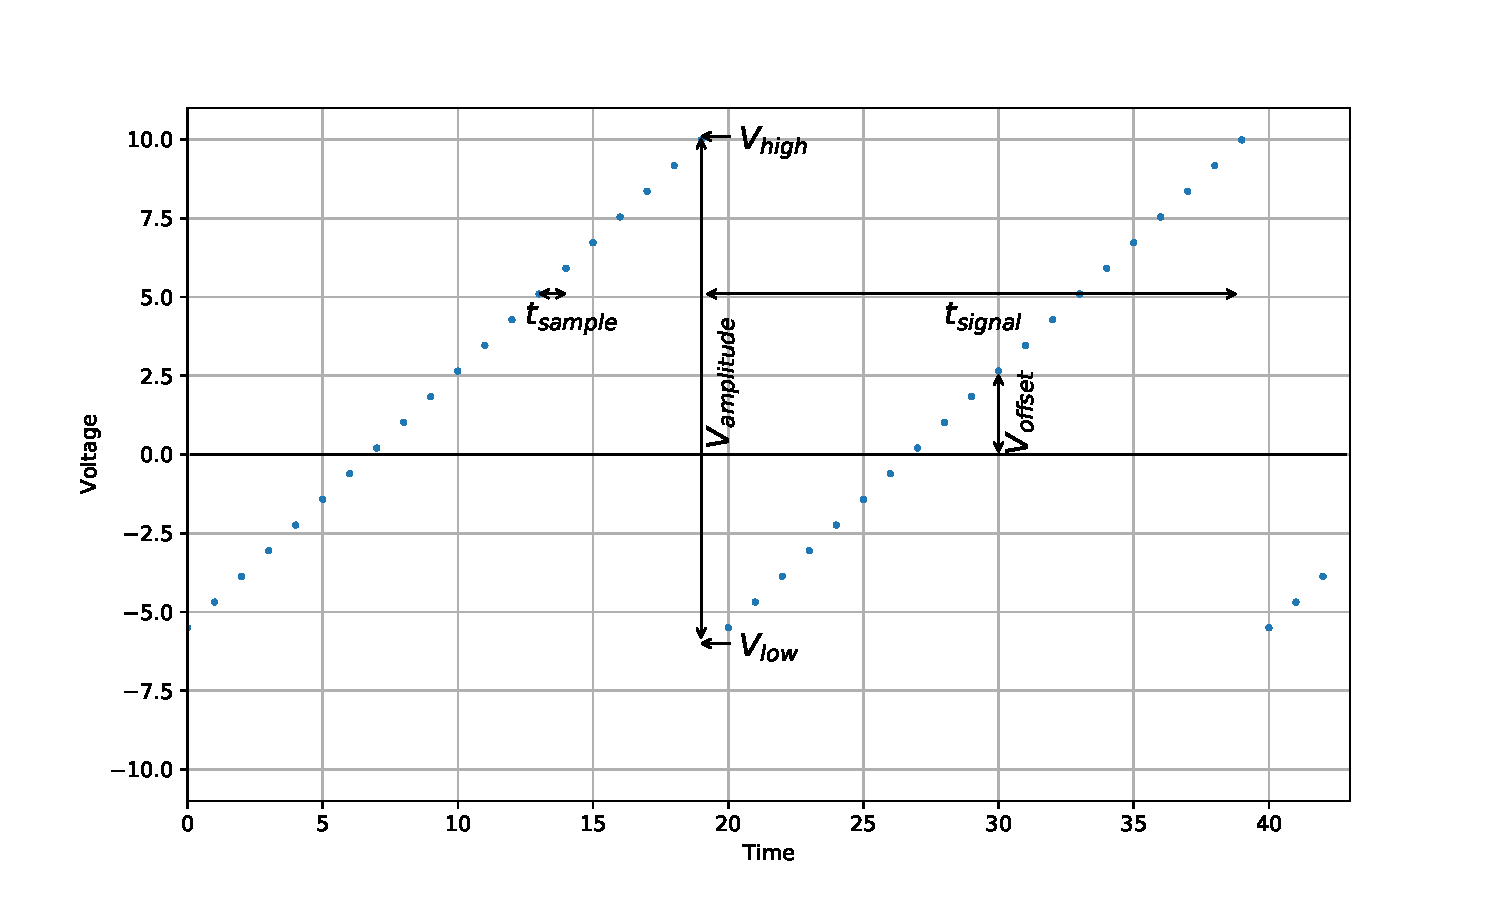
\includegraphics[width=0.99\textwidth, trim = {0 1.6cm 0 1.5cm}, clip]{src/_rampProperties.pdf}
	\end{center}
	\begin{align*}
	t_{sample} &\textrm{ ... sampling-time or -period, alias: trigger-rate } \\
	t_{signal} &\textrm{ ... signal-time or -period } \\
	f_{sample} &\textrm{ ... sampling-frequency or -rate } \\
	f_{signal} &\textrm{ ... signal-frequency or -rate } \\
	N &\textrm{ ... sample-count, length of the signal-vector } \\
	f_{sample} & = \frac{1}{t_{sample}} = N \cdot f_{signal} \\
	f_{signal} & = \frac{1}{t_{signal}} = \frac{1}{N \cdot t_{sample}} \\
	% f_{sample} & = N \times f_{signal} \\
	% t_{signal} & = N \times t_{sample}	\\
	% \end{align*}
	% \begin{align*}
	V_{amplitude} &\textrm{  ... difference between maximum and minimum voltage of a signal. } \\
	V_{offset} &\textrm{  ... deviation of a signal from 0 volts. } \\
	V_{high} &\textrm{  ... maximum voltage of a signal } \\
	V_{low} &\textrm{  ... minimum voltage of a signal } \\
	V_{amplitude} &= V_{high} - V_{low} \\ % \quad \quad V_{high} = V_{offset} + \frac{V_{amplitude}}{2} \\
	V_{offset} &= \frac{V_{high} + V_{low}}{2} \\ % \quad \quad V_{low} = V_{offset} - \frac{V_{amplitude}}{2} \\
	\rightarrow V_{high} &= V_{offset} + \frac{V_{amplitude}}{2} \quad V_{low} = V_{offset} - \frac{V_{amplitude}}{2}
	\end{align*}
	
	
	\req{ RI-5 }{Priorities}{}{}
	{ In case of temporal overlapping tasks, first priority lays with analogue signal generation, second prio with USB-connectivity, third prio with Miscellaneous functions. }
	{}{}{}{General}

	
	\req{ RU-2  }{Last Command Counts}{}{}
	{ The last submitted and accepted value for each parameter is the valid one.}
	{}{}{}{General}

	\req{ RU-3  }{Parameters}{}{}
	{ The FirmWare has to implement user-adjustable parameters according to Tab. 1. }
	{}{}{}{General}
	
	{	\scriptsize
					\begin{table}[H]
			\centering
			\scriptsize
			\begin{tabular}{l|p{65mm}|l|l|l}
			% \hline
			\redrow Parameter 	& Values						& reset value 	& Dim.		& Type 	\\ \hline
			TriggerA State		& off|idle|arm|run				& idle			& 			& enum	\\ \hline
			TrigA Mode			& finite|infinite (freerun)		& finite		& 			& enum	\\ \hline
			TrigA Input			& USB|ext|TrigB|butt0 			& TrigB			& 			& enum	\\ \hline
			TrigA Signal-Rate	& 100m ... 125k					& 30.00e3		& Hz		& float	\\ \hline
			TrigA Signal-Period	& 8u ... 10						& 3.33e-5		& s			& float	\\ \hline
			TrigA Size			& 0	... 250000	 				& 1000			& samples	& int	\\ \hline
			TriggerB State		& off|idle|arm|run 				& idle			& 			& enum	\\ \hline
			TrigB Signal-Rate	& 100m ... 125k					& 30			& Hz		& float	\\ \hline
			TrigB Mode			& finite|infinite (freerun)		& finite		& 			& enum	\\ \hline
			TrigB Input			& USB|ext|TrigC|butt1 			& TrigC			& 			& enum	\\ \hline
			TrigB Signal-Period	& 8u ... 10						& 3.33e-2		& s			& float	\\ \hline
			TrigB Size			& 0	... 250000	 				& 1000			& samples	& int	\\ \hline
			TriggerC State		& off|idle|arm|run				& idle			& 			& enum	\\ \hline
			TrigC Mode			& finite|infinite (freerun)		& finite		& 			& enum	\\ \hline
			TrigC Input			& USB|ext|butt2					& USB			& 			& enum	\\ \hline
			TrigC Signal-Rate	& 20m ... 125k					& 3e-2			& Hz		& float	\\ \hline
			TrigC Signal-Period	& 8u ... 50						& 33.33			& s			& float	\\ \hline
			TrigC Size			& 0 ... 250000					& 1				& samples	& int	\\ \hline
			SourceA Mode		& triggered|detached|singleshot	& triggered		& -			& enum	\\ \hline
			SourceA Function	& ramp|arbitrary 				& ramp			& -			& enum	\\ \hline
			SourceA Symmetry	& 	0 ... 100					& 0				& percent	& float	\\ \hline
			SourceA Amplitude	& 	0 ... 20					& 20			& volts		& float	\\ \hline
			SourceA Offset		& -10 ... +10					& 0				& volts		& float	\\ \hline
			SourceA High-Volt	& -10 ... +10					& +10			& volts		& float	\\ \hline
			SourceA Low-Volt	& -10 ... +10					& -10			& volts		& float	\\ \hline
			SourceA Const-Volt	& -10 ... +10					& 0				& volts		& float	\\ \hline
			SourceA timeout		& 0 ... 1000					& 0				& ms		& float	\\ \hline
			SourceB Mode		& triggered|detached|singleshot	& triggered		& -			& enum	\\ \hline	
			SourceB Function	& ramp|arbitrary				& ramp			& -			& enum	\\ \hline	
			SourceB Symmetry	& 0	... 100						& 0				& percent	& float	\\ \hline
			SourceB Amplitude	& 0	...  20						& 20			& volts		& float	\\ \hline
			SourceB Offset		& -10 ... +10					& 0				& volts		& float	\\ \hline
			SourceB High-Volt	& -10 ... +10					& +10			& volts		& float	\\ \hline
			SourceB Low-Volt	& -10 ... +10					& -10			& volts		& float	\\ \hline
			SourceB Const-Volt	& -10 ... +10					& 0				& volts		& float	\\ \hline
			SourceB timeout		& 0 ... 1000					& 0				& ms		& float	\\ \hline
			I2C mode    	   	& off|USB|slave 				& off			& -			& enum	\\ \hline
			UART mode	     	& off|USB|slave 				& off			& -			& enum	\\ \hline
			Galvo-Relay			& off|on						& off			& -			& bool	\\ \hline
			SLD-Relay			& off|on						& off			& -			& bool	\\ \hline
			AIM-Relay			& off|on						& off			& -			& bool	\\ \hline
			CAM-Relay			& off|on						& off			& -			& bool	\\ \hline
			Relay5				& off|on						& off			& -			& bool	\\ \hline
			Relay6				& off|on						& off			& -			& bool	\\ \hline
			Watchdog			& off|reset|powerdown|keepalive &				& -			& enum	\\ \hline
			WDGTimeout			& 0 ... 1000					& 1000			& ms		& int	\\ \hline
			CRCmode				& off|on						& off			& -			& bool	\\ \hline
			VerboseMode			& off|on						& on			& -			& bool	\\ \hline
			A-in mode			& off|USB|trig'd 				& -				& -			& enum	\\ \hline
			A-in value			& 0 ... $2^{12}$				& -				& LSB		& int	\\ \hline
			D-IO mode			& off|in|out 					& -				& -			& enum	\\ \hline
			D-IO value			& 0 ... $2^{16}$				& -				& bin-vect	& int	\\ \hline
					\end{tabular}
				\caption{user-adjustable parameters}
			\label{tab:params}
		\end{table}


	}





	\req{ RU-4 }{USB-Protocol}{ H }{ WIP }
	{  The device has to provide the user with a USB-Interface. It has to be in the form of a VCP, text-based and SCPI-oriented.
		Messages in either direction may be up to 100 characters long and have to be delimited by the linefeed symbol '\texttt{\textbackslash}n'.	}
	{}{}{}{USB-Stack}
	\req{ RU-5  }{USB-Actions}{ H }{ WIP }
	{ The FirmWare has to perform actions and state transitions as requested by USB-messages.}
	{}{}{}{USB-Stack}
	\req{ RU-6 }{Verbose}{}{}
	{ The FW has to reply to every USB-command with a meaningful answer. This is called a 'verbose'-mode, has to be active on startup, but detachable by SCPI-command. Opposite is called $laconic$ - mode }
	{}{}{}{USB-Stack}
	\req{ RU-7 }{USB-Timing}{}{}
	{ USB-messages sent from the device to the host must be sent with a minimum interval of 1ms. The device must receive USB-messages in intervals up to 1ms.}
	{}{}{}{USB-Stack}
	\req{ RU-8  }{Case-Insensitivity}{ M }{ WIP }
	{  The SCPI-detection has to be case-insensitive, and respond to the long form as well as the short form of SCPI commands.}
	{}{}{}	{USB-Stack}
	\req{ RU-9  }{USB-turnoff}{}{}
	{	The FirmWare has to deactivate USB-reactivity during  A-, B- or C-scans, unless in freerun-mode.
		On startup, this functionality is active.	}
	{}{}{}{USB-Stack}
	\req{ RU-10  }{SCPI}{ H }{ WIP }
	{ The FirmWare has to parse USB-messages in a SCPI-fashion as defined in document "USB-Protocol.pdf", into FW-internal data structures.}
	{}{}{}{USB-Stack}
	\req{ RU-11  }{Restart}{ H }{ WIP }
	{ The FirmWare has to perform a complete System-restart, when requested by USB-command.}
	{}{}{}{USB-Stack}
	\req{ RU-12  }{Standard-SCPIs}{}{}
	{ The FirmWare has to implement mandatory SCPI-command according to IEEE 488.2}
	{}{}{}{USB-Stack}


	\req{ RU-13  }{Arbitrary Signal Vectors}{}{}
	{The FirmWare must provide functionality to load user-defined arbitrary signal vectors, individually for both channels. 
		In $verbose$ - mode, every single transmitted value will be replied with a meaningful message, in $laconic$ - mode, only the average value of the final vector will be replied
		Values will be transmitted one value per USB-command. optional: Transmit-mode to submit values chunk-wise.	}
	{}{}{}{Signals}
	\req{ RU-14  }{Vector Length}{}{}
	{ The FirmWare must provide functionality to set a user-defined signal vector length, either for ramp- and arbitrary signal, individually for both channels. }
	{}{}{}{Signals}
	\req{ RU-15  }{source states}{}{}
	{ Signal generation must contain the following operational modes:  $triggered$, $detached$, $single-shot$
		\begin{itemize}
		\item $triggered$ : each pulse of the corresponding trigger causes the next vector value to be represented at the analogue output (default)
		\item $detached$ : analogue output holds a certain constant level, regardless of trigger and vector values ( alias: $ref-pos$ - mode )
		\item $single-shot$ : analogue output holds a certain constant level, and returns to 0 volt after a specified timeout.
		\end{itemize}	}
	{}{}{}{Signals}
	\req{ RU-16  }{Default Ramp Signals}{}{}
	{ By default, signal vectors are to be loaded with ramp signals.}
	{}{}{}{Signals}
	\req{ RU-17  }{signal-end}{}{}
	{ The FirmWare has to stop signal generation upon completion of all vector lengths and reset analogue outputs to 0V. }
	{}{}{}{Signals}
	\req{ RU-18  }{free-run}{}{}
	{ The FirmWare has to provide a freerun mode. This mode continues signal generation, until a specific stop command is submitted via USB.}
	{}{}{}{Signals}
	\req{ RU-19  }{Adjustable Signal Parameters}{}{}
	{ Signal generation has to be adjustable in amplitude and offset  {\bf or}  high and low-voltage, signal-freq, {\bf or} -period ). This values apply to ramp- as well as arbitrary signals and will be applied to the signal vectors in a overwriting manner. }
	{}{}{}{Signals}
	\req{ RU-20  }{Ramp symmetry}{}{}
	{Ramp signals must have adjustable symmetry/asymmetry between 0$\%$ and 100$\%$. The according meaning is depicted in the following graphics. }
	{}{}{}{Signals}
		\begin{center}
		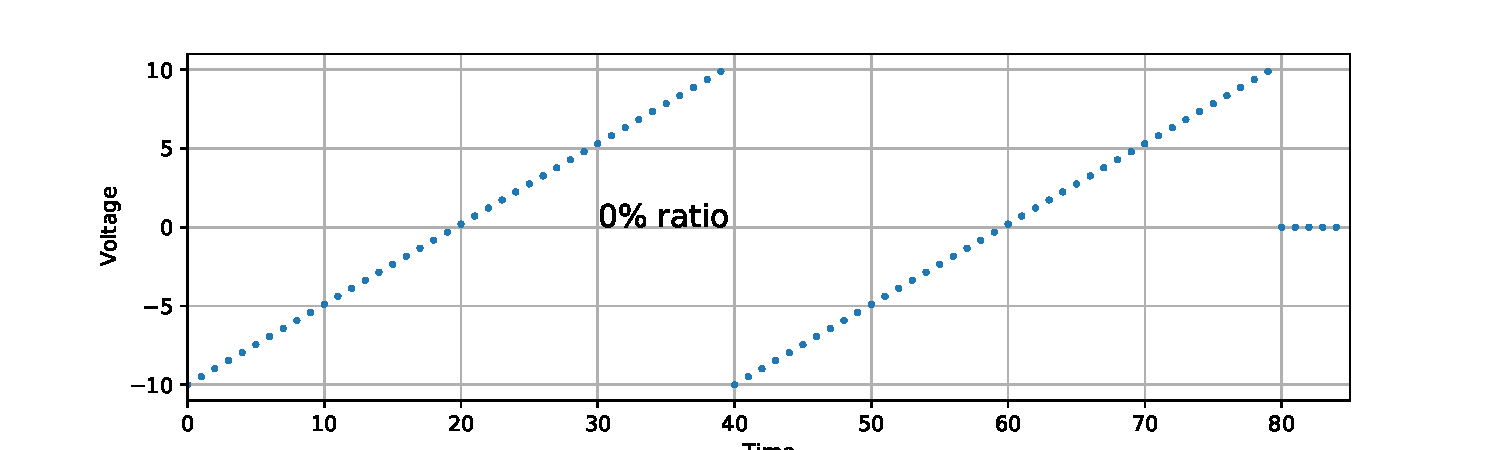
\includegraphics[width=0.95\textwidth]{src/_rampAssymetry0perc.pdf}
		\end{center}
		\begin{center}
		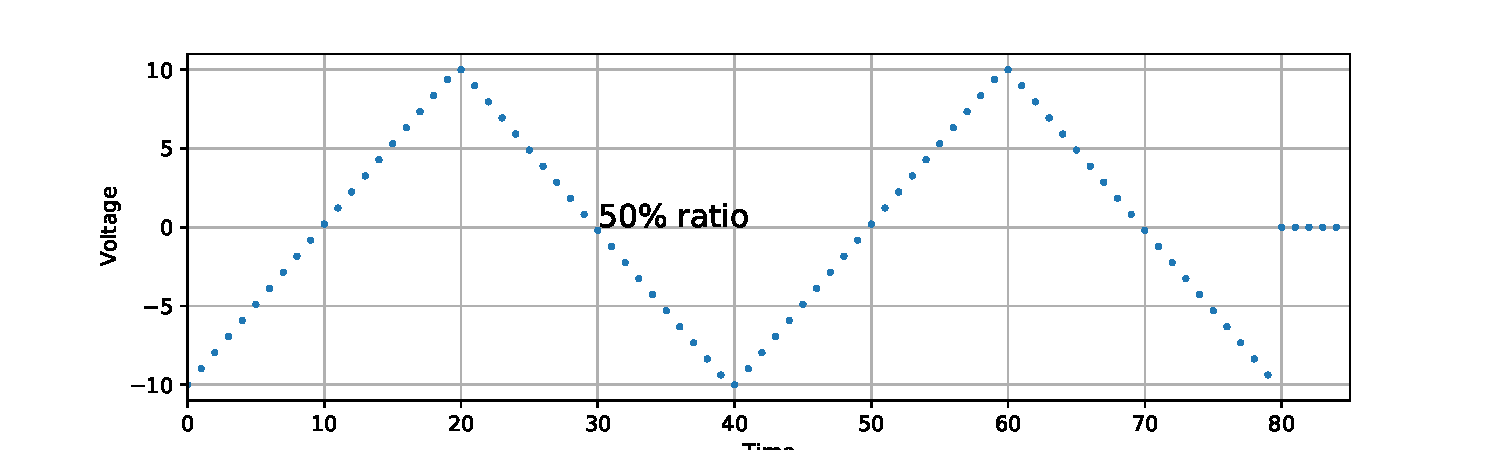
\includegraphics[width=0.95\textwidth]{src/_rampAssymetry50perc.pdf}
		\end{center}
		\begin{center}
		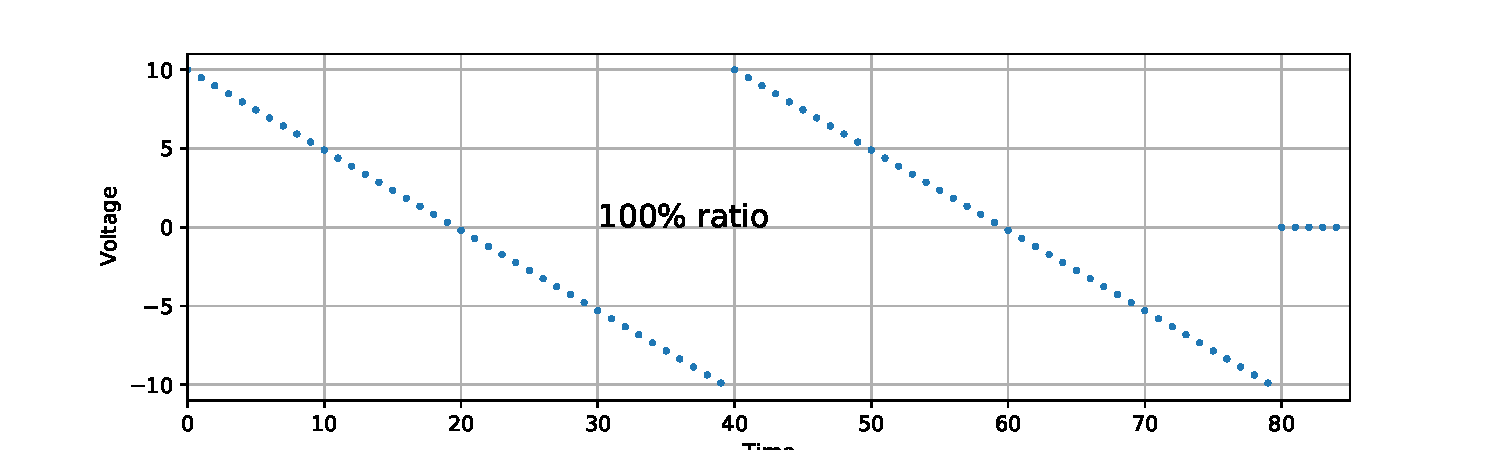
\includegraphics[width=0.95\textwidth]{src/_rampAssymetry100perc.pdf}
		\end{center}


	\req{ RU-21  }{Trigger-IO}{}{}
	{ Internal Trigger-Pulses must be put out via corresponding Trigger-outputs }
	{}{}{}{Triggers}
	\req{ RU-22  }{Trigger-Source}{}{}
	{ Trigger-Modules must be implemented to handle timing of the signal-generation, comprising following input-sources:  $USB$, $Trigger-Input$, $Superior$-$Trigger$, $Push-button$ }
	{}{}{}{Triggers}
	\req{ RU-23  }{Timing-Parameters}{}{}
	{ The FirmWare has to accept signal frequency or signal period and signal vector length as parameters. It has to reply with the actual frequency/period or an error message.}
	{}{}{}{Triggers}
	\req{ RU-24  }{Timing-Calc}{}{}
	{ The FirmWare has to derive necessary sample-rates and trigger-periods from signal period and vector length, either by calculation or by selection from a look-up-table.}
	{}{}{}{Triggers}
	\req{ RU-25  }{Sequences}{}{}
	{ The FirmWare has to generate sequences of A, B and C-Triggers. A-Trigger pulses have a duty-cycle of 50\%, B and C-Trigger have falling edges upon completion.}
	{}{}{}{Triggers}
		\begin{center}
		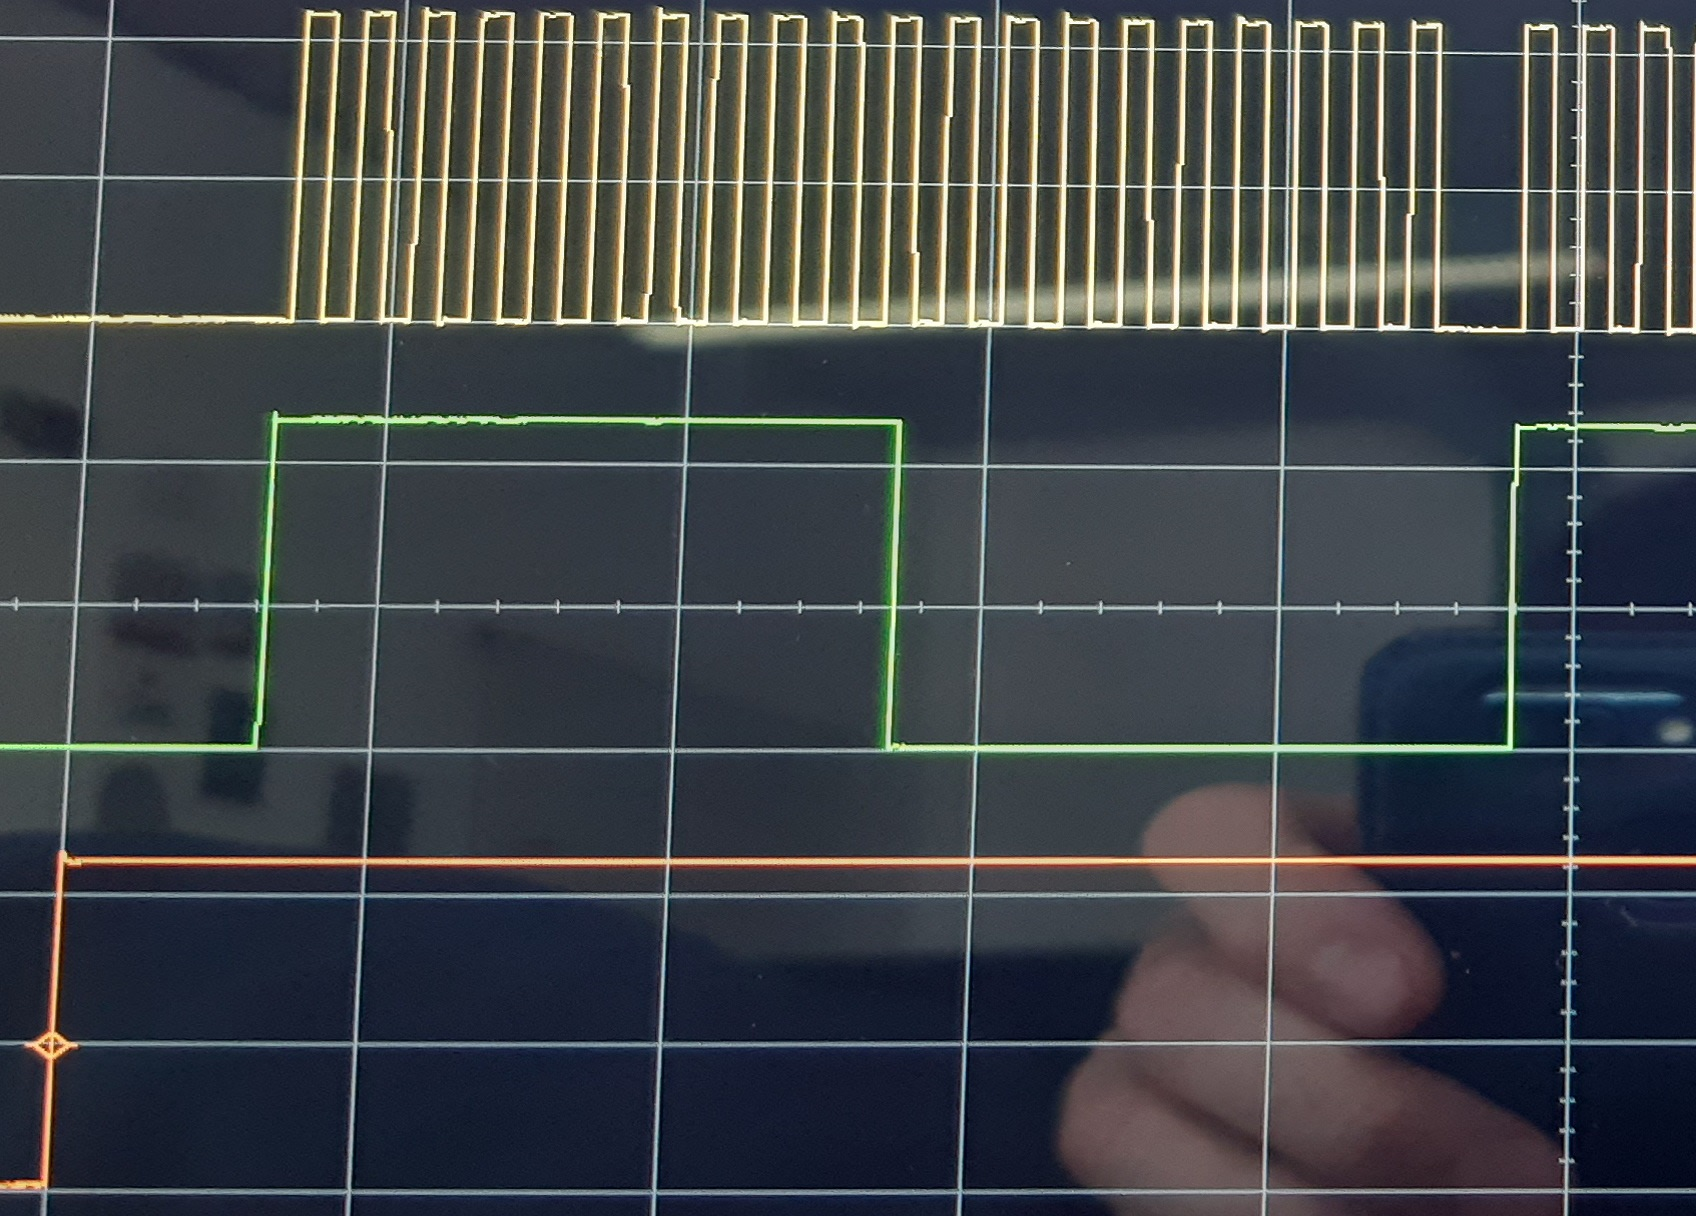
\includegraphics[height=0.2\textheight]{src/_TrigSequence.jpg}
		\end{center}


	\req{ RU-26  }{Buttons,LEDs}{}{}
	{ The FirmWare must access the available push-buttons and state-LEDs. }
	{}{}{}{Miscellaneous}
	\req{ RU-27  }{Button-Function}{}{}
	{ Push-buttons must be programmed to cause transitions to the devices internal state, in a debounced manner. }
	{}{}{}{Miscellaneous}
	\req{ RU-28  }{LED-Function}{}{}
	{ State-LEDs have to represent the current internal state of the device: $idle$, $armed$, $running$ or $error$. }
	{}{}{}{Miscellaneous}
	\req{ RU-29 }{Relays}{}{}
	{ The FirmWare has to provide access to the available relays. Access must consist of $close$, $open$ and $read$-functions }
	{}{}{}{Miscellaneous}
	\req{ RU-30 }{Additional IOs}{}{}
	{ The FirmWare has to provide access for available UART-, $I^2C$-, SPI-modules, as well as digital IOs and analogue inputs.}
	{}{}{}{Miscellaneous}
	\req{ RU-31 }{Additional IO-Modes}{}{}
	{ Functionality for USART-, $I^2C$-, SPI-modules, the digital IOs and analogue inputs must consist of $activation$, $de-activation$, $write$ and $read$.}
	{}{}{}{Miscellaneous}
	\req{ RU-32 }{IO Read}{}{}
	{ $read$-Function must send received information to the host via USB.
	  $read$-Function must be performed upon USB-command, or slave-action.}
	{}{}{}{Miscellaneous}
	\req{ RU-33  }{CRC}{}{}
	{ The FirmWare has to implement functions to perform cyclic-redundancy-check calculations and apply it on verification of incoming strings and adaption of outgoing strings}
	{}{}{}	{Miscellaneous}
	\req{ RU-34  }{Watchdog Functionality \label{WDG}}{ M }{ todo }
	{  The FirmWare has to implement functions to enable the processors built-in watchdog and set its parameters. Available modes have to be $reset$, $powerdown$, $keepalive$}
	{}{}{}	{Miscellaneous}



		\pagebreak
			\subsection{USB-Protocol}
		A direct consequence of the user-requirements is the list of scpi-commands and according replies, forming the USB-protocol.	Scpi-commands can be in 'short form', defined by the capital letters, or in 'long form', defined by the whole string. OCTane accepts both forms as commands and is case-insensitive. \cite{scpi1993}
		{	\scriptsize
					\begin{longtable}{|l|l|l|l|l|}				\hline
		Sub-sys				& Parameter		& Value					& Command									& Response 			\\ \hline
		\redrow	Trigger A	& State			& off|idle|arm|run		& TRIGgerA:STATe	OFF						& <state>|<error>	\\ \hline
							& State			& 						& TRIGgerA:STATe	IDLE					& <state>|<error>	\\ \hline
							& State			& 						& TRIGgerA:STATe	ARM						& <state>|<error>	\\ \hline
							& State			& 						& TRIGgerA:STATe	RUN						& <state>|<error>	\\ \hline
							& Mode (freerun)& finite				& TRIGgerA:MODE		FINite					& <mode> |<error>	\\ \hline
							& Mode 			& infinite				& TRIGgerA:MODE		INFinite				& <mode> |<error>	\\ \hline
							& Input			& USB					& TRIGgerA:INput	USB						& <input>|<error>	\\ \hline
							& Input			& external input		& TRIGgerA:INput	EXTernal				& <input>|<error>	\\ \hline
							& Input			& Trigger B				& TRIGgerA:INput	TRIGgerB				& <input>|<error>	\\ \hline
							& Input			& Trigger C				& TRIGgerA:INput	TRIGgerC				& <input>|<error>	\\ \hline
							& Input			& Button				& TRIGgerA:INput	BUTTon					& <input>|<error>	\\ \hline
							& Signal-Rate	& 1.0e-1 ... 125e3		& TRIGgerA:RATE		<freq>					& <time>|<error>	\\ \hline
							& Signal-Period	& 	8e-6	... 10		& TRIGgerA:PERIod	<time>					& <time>|<error>	\\ \hline
							& Vector-Size	& 1...250000			& TRIGgerA:SIZE		<size>					& <size>|<error>	\\ \hline
		%	Sequencer		& -Gener		& 						& TRIGgerA:									& DONE|		\\ \hline
		\redrow	Trigger B	& State			& off|idle|arm|run		& TRIGgerB:STATe	OFF						& <state>|<error>	\\ \hline
							& State			& 						& TRIGgerB:STATe	IDLE					& <state>|<error>	\\ \hline
							& State			& 						& TRIGgerB:STATe	ARM						& <state>|<error>	\\ \hline
							& State			& 						& TRIGgerB:STATe	RUN						& <state>|<error>	\\ \hline
							& Mode (freerun)& finite				& TRIGgerB:MODE		FINite					& <mode> |<error>	\\ \hline
							& Mode 			& infinite				& TRIGgerB:MODE		INFinite				& <mode> |<error>	\\ \hline
							& Input			& USB					& TRIGgerB:INput	USB						& <input>|<error>	\\ \hline
							& Input			& External				& TRIGgerB:INput	EXTernal				& <input>|<error>	\\ \hline
							& Input			& Trigger C				& TRIGgerB:INput	TRIGgerC				& <input>|<error>	\\ \hline
							& Input			& Button				& TRIGgerB:INput	BUTTon					& <input>|<error>	\\ \hline
							& Signal-Rate	& 	1.0e-1 ... 125e3	& TRIGgerB:RATE		<freq>					& <time>|<error>	\\ \hline
							& Signal-Period	& 	8e-6	... 10		& TRIGgerB:PERIod	<time>					& <time>|<error>	\\ \hline
							& Vector-Size	& 1...250000			& TRIGgerB:SIZE		<size>					& <size>|<error>	\\ \hline
		%	Sequencer		& -Gener		& 						& TRIGgerB:									& DONE|		\\ \hline
		\redrow	Trigger C	& State			& off|idle|arm|run		& TRIGgerC:STATe	OFF						& <state>|<error>	\\ \hline
							& State			& 						& TRIGgerC:STATe	IDLE					& <state>|<error>	\\ \hline
							& State			& 						& TRIGgerC:STATe	ARM						& <state>|<error>	\\ \hline
							& State			& 						& TRIGgerC:STATe	RUN						& <state>|<error>	\\ \hline
							& Mode (freerun)& finite				& TRIGgerC:MODE		FINite					& <mode> |<error>	\\ \hline
							& Mode 			& infinite				& TRIGgerC:MODE		INFinite				& <mode> |<error>	\\ \hline
							& Input			& USB					& TRIGgerC:INput	USB						& <input>|<error>	\\ \hline
							& Input			& External				& TRIGgerC:INput	EXTernal				& <input>|<error>	\\ \hline
							& Input			& Button				& TRIGgerC:INput	BUTTon					& <input>|<error>	\\ \hline
							& Signal-Rate	& 	1.0e-1 ... 125e3	& TRIGgerC:RATE		<freq>					& <time>|<error>	\\ \hline
							& Signal-Period	& 	8e-6	... 10		& TRIGgerC:PERIod	<time>					& <time>|<error>	\\ \hline
							& Vector-Size	& 1...250000			& TRIGgerC:SIZE		<size>					& <size>|<error>	\\ \hline
						% 	& Slope			& rising|falling Edge	& TRIGgerC:SLOPe	<POS|NEG>				& DONE|		\\ \hline
						% 	& Outmode		& pulse|duty			& TRIGgerC:OUTMode	<pulse|duty>			& DONE|		\\ \hline
						% 	& Outpulse		& pulse|duty			& TRIGgerC:OUTPulse	<time>					& DONE|		\\ \hline
						% 	& OutSlope		& rising|falling Edge	& TRIGgerC:OUTSLope	<POS|NEG>				& DONE|		\\ \hline
		%	Sequencer		& -Gener		& 						& TRIGgerC:									& DONE|		\\ \hline
		\redrow	Source-A	& Mode			& triggered				& SOURceA:MODE			TRIGgered			& <mode>|<error> 	\\ \hline
							& Mode			& detached				& SOURceA:MODE			DETached			& <mode>|<error> 	\\ \hline
							& Mode			& singleshot			& SOURceA:MODE			SINGleshot			& <mode>|<error> 	\\ \hline
							& Function		& Ramp					& SOURceA:FUNCtion:SHAPe 	RAMP	 		& <func>|<error>	\\ \hline
							& Function		& 		Arbitrary		& SOURceA:FUNCtion:SHAPe 	ARBitrary 		& <func>|<error>	\\ \hline
							& Symmetry		& 0 ... 100 			& SOURceA:RAMP:RATIO 	<ratio> 			& <ratio>|<error> 	\\ \hline
							& Arb load		& -						& SOURceA:ARBitrary:LOAD 					& <count>|<error>	\\ \hline
							& Arb val		& $\pm$10.000			& SOURceA:ARBitrary:VALUe <idx, val>		& <idx, val>|<error>\\ \hline
							& Amplitude		& 0.000...20.000		& SOURceA:FUNCtion:AMPlitude <ampl>			& <ampl>|<error>	\\ \hline
							& Offset		& $\pm$10.000			& SOURceA:FUNCtion:OFFset <offs>			& <offs>|<error>	\\ \hline
							& High			& $\pm$10.000			& SOURceA:FUNCtion:HIgh <high>				& <high>|<error>	\\ \hline
							& Low			& $\pm$10.000			& SOURceA:FUNCtion:LOw <low>				& <low>|<error> 	\\ \hline
							& Constant		& $\pm$10.000			& SOURceA:VOLTage:LEVel	<volts>				& <volts>|<error> 	\\ \hline
							& Timeout		&  1...1000ms		 	& SOURceA:PULSe:WIDth		<time>			& <time>|<error> 	\\ \hline
						% 	& ReadVec		& -						& SOURceA:ARBitrary:READ					& all vector values \\ \hline
		\redrow	Source-B	& Mode			& trig|det|single		& SOURceB:MODE			TRIGgered			& <mode>|<error> 	\\ \hline
							& Mode			& trig|det|single		& SOURceB:MODE			DETached			& <mode>|<error> 	\\ \hline
							& Mode			& trig|det|single		& SOURceB:MODE			SINGleshot			& <mode>|<error> 	\\ \hline
							& Function		& Ramp					& SOURceB:FUNCtion:SHAPe 	RAMP	 		& <func>|<error>	\\ \hline
							& Function		& Arbitrary				& SOURceB:FUNCtion:SHAPe 	ARBitrary 		& <func>|<error>	\\ \hline
							& Symmetry		& 0 ... 100 			& SOURceB:RAMP:RATIO 	<ratio> 			& <ratio>|<error> 	\\ \hline
							& Arb load		& -						& SOURceB:ARBitrary:LOAD 					& <count>|<error>	\\ \hline
							& Arb val		& $\pm$10.000			& SOURceB:ARBitrary:VALUe <idx, val> 		& <idx, val>|<error>\\ \hline
							& Amplitude		& 0.000...20.000		& SOURceB:FUNCtion:AMPlitude <ampl>			& <ampl>|<error>	\\ \hline
							& Offset		& $\pm$10.000			& SOURceB:FUNCtion:OFFset <offs>			& <offs>|<error>	\\ \hline
							& High			& $\pm$10.000			& SOURceB:FUNCtion:HIgh <high>				& <high>|<error>	\\ \hline
							& Low			& $\pm$10.000			& SOURceB:FUNCtion:LOw <low>				& <low>|<error> 	\\ \hline
							& Constant		& $\pm$10.000			& SOURceB:VOLTage:LEVel	<volts>				& <volts>|<error> 	\\ \hline
							& Timeout		&  1...1000ms		 	& SOURceB:PULSe:WIDth		<time>			& <time>|<error> 	\\ \hline
						% 	& ReadVec		& -						& SOURceB:ARBitrary:READ					& all vector values \\ \hline
		% \redrow	Misc.		& 				& 						& 											&  					\\ \hline
			Relays			& Galvo			& close|open|read		& ROUTe:<CLOSe|OPEN|STATE?> GAL				& <state>|<error>	\\ \hline
							& SLD			& close|open|read		& ROUTe:<CLOSe|OPEN|STATE?> SLD				& <state>|<error>	\\ \hline
							& AIM			& close|open|read		& ROUTe:<CLOSe|OPEN|STATE?> AIM				& <state>|<error>	\\ \hline
							& CAM			& close|open|read		& ROUTe:<CLOSe|OPEN|STATE?> CAM				& <state>|<error>	\\ \hline
						% 	& Sense			& read state			& ROUTe:STATE?	GAL|SLD|AIM|CAM				& <state>|<error>	\\ \hline
						% 	& close			& close Relay			& ROUTe:CLOSe	GAL|SLD|AIM|CAM				& <state>|<error>	\\ \hline
						% 	& open			& open Relay			& ROUTe:OPEN	GAL|SLD|AIM|CAM				& <state>|<error>	\\ \hline
			I2C				& mode			& OFF					& I2C::MODE OFF								& <mode>|<error>	\\ \hline
							& mode			& USB					& I2C::MODE USB								& <mode>|<error>	\\ \hline
							& mode			& slave-action			& I2C::MODE SLAVeaction						& <mode>|<error>	\\ \hline
							& write			& 0 ... 255				& I2C::WRITe <val>							& <val>|<error> 	\\ \hline
							& read			& 0 ... 255				& I2C::READ									& <val>|<error> 	\\ \hline
			UART			& mode			& OFF					& UART:MODE OFF								& <mode>|<error> 	\\ \hline
							& mode			& USB					& UART:MODE USB								& <mode>|<error> 	\\ \hline
							& mode			& slave-IRQ				& UART:MODE SLAVeaction						& <mode>|<error> 	\\ \hline
							& write			& 0 ... 255				& UART:WRITe <val>							& <val>|<error>		\\ \hline
							& read			& 0 ... 255				& UART:READ									& <val>|<error> 	\\ \hline
			DIO				& mode			& OFF			 		& DIGIO:MODE OFF							& <val>|<error>		\\ \hline
							& mode			& input			 		& DIGIO:MODE IN								& <val>|<error>		\\ \hline
							& mode			& output 				& DIGIO:MODE OUT							& <val>|<error>		\\ \hline
							& write			& 0 .. 65535			& DIGIO:WRIte <val>							& <val>|<error>		\\ \hline
							& read			& 0 .. 65535			& DIGIO:READ								& <val>|<error>		\\ \hline
			AnalogIN		& mode			& OFF					& ANAlog0|1|2|3:MODE OFF					& <val>|<error>		\\ \hline
							& mode			& USB					& ANAlog0|1|2|3:MODE USB					& <val>|<error>		\\ \hline
							& mode			& triggered				& ANAlog0|1|2|3:MODE TRIGA					& <val>|<error>		\\ \hline
							& mode			& triggered				& ANAlog0|1|2|3:MODE TRIGB					& <val>|<error>		\\ \hline
							& mode			& triggered				& ANAlog0|1|2|3:MODE TRIGC					& <val>|<error>		\\ \hline
							& read			& 0 ... 4095			& ANAlog0|1|2|3:READ						& <val>|<error>		\\ \hline
		\redrow System		& CRCmode		& OFF					& SYStem:CRC16 OFF							& <state>|<error>	\\ \hline
							& CRCmode		& on					& SYStem:CRC16 ON							& <state>|<error>	\\ \hline
							& ShutDown 		& -						& SYStem:POWerdown							& POWD|<error>	\\ \hline
							& ListSCPI 		& -						& SYStem:LISt								& <list>|<error>	\\ \hline
							& RESEt 		& -						& SYStem:RESEt								& RESE|<error>		\\ \hline
							& RESTart 		& -						& SYStem:RESTart							& REST|<error>	\\ \hline
							& Verbosity		& OFF					& SYStem:VERBose OFF						& <mode>|<error>	\\ \hline
							& Verbosity		& on					& SYStem:VERBose ON							& <mode>|<error>	\\ \hline
							& Watchdog		& OFF					& SYStem:WATchdog OFF						& <mode>|<error>	\\ \hline
							& Watchdog		& on					& SYStem:WATchdog ON						& <mode>|<error>	\\ \hline
							& Time			& 1...1000ms			& SYStem:WATchdog <time>					& <time>|<error>	\\ \hline
			% Encoder		& 	opt. 		& 						& 												& 		& 		\\ \hline
			% Stepper		& 	opt. 		& 						& 												& 		& 		\\ \hline
		\caption{OCTane USB-Protocol, commands}
			\end{longtable}

		% \begin{table}[h!]
			\centering
			\begin{longtable}{|l|l|l|l|l|l|}
			% \begin{tabular}{|p{1.6cm}|l|l|l|l|l|}
			\hline


		Sub-sys					&  Parameter	 	& possible messages	& occurence 						& 			&  \\ \hline
		\redrow	Trigger A|B|C	&  State	 		& TrigX idling|armed|running& sent on every state change 		& 			& 	\\ \hline
				Trigger A|B|C 	& Input				& -200				& error, if button in use			& 			& 	\\ \hline
				Trigger A|B|C 	& Signal-Rate		& -200				& error, if out-of-range			& 			& 	\\ \hline
				Trigger A|B|C 	& Signal-Period		& -200				& error, if out-of-range			& 			& 	\\ \hline
				Trigger A|B|C 	& Vector-Size		& -200				& error, if out-of-range			& 			& 	\\ \hline
		\redrow	Source A|B		& Arb load	 		& -200				& error, if not in Arb-mode			& 			& 	\\ \hline
				Source A|B		& Arb val	 		& VectorX complete	& if sufficient amount of values was sent	& 			& 	\\ \hline
				Source A|B		& Arb val	 		& -200				& error, if out-of-range			& 			& 	\\ \hline
				Source A|B		& Arb val	 		& -200				& error, if exeeds vector-size		& 			& 	\\ \hline
				Source A|B		& Symmetry	 		& -200				& error, if out-of-range			& 			& 	\\ \hline
				Source A|B		& Amplitude			& -200				& error, if out-of-range			& 			& 	\\ \hline
				Source A|B		& Offset			& -200				& error, if out-of-range			& 			& 	\\ \hline
				Source A|B		& High				& -200				& error, if out-of-range			& 			& 	\\ \hline
				Source A|B		& Low				& -200				& error, if out-of-range			& 			& 	\\ \hline
				Source A|B		& Constant			& -200				& error, if out-of-range			& 			& 	\\ \hline
				Source A|B		& Timeout			& -200				& error, if out-of-range			& 			& 	\\ \hline

		\redrow	AIN 			& input value		& AINx: <value>		& sent on every corresp. Trigger	& 			& 	\\ \hline
				DIN 			& input value		& DIN: <value>		& sent on every DIO:READ-Command	& 			& 	\\ \hline
				UART 			& input value		& UART: <value>		& sent on every corresp. Trigger	& 			& 	\\ \hline
				I2C 			& input value		& I2C: <value>		& sent on every corresp. Trigger	& 			& 	\\ \hline
		\caption{OCTane USB-Protocol, responses}
		\label{USB-Protocol-responses}
		\end{longtable}
		% \end{table}

		}
		Table ~\ref{USB-Protocol-responses} specifies the responses by the OCTane, if they are not described sufficiently in the previous table.
		{	\scriptsize
					\begin{longtable}{|l|l|l|l|l|}				\hline
			Command & 	Description									& 	Action	& Return		\\ \hline
			*CLS	& Clear Status Command							& 		& 		\\ \hline
			*ESE & Standard Event Status Enable Command	& 		& 		\\ \hline
			*ESE? & Standard Event Status Enable Query 		& -		& 		\\ \hline
			*ESR? & Standard Event Status Register Query 	& -		& 		\\ \hline
			*IDN? & Identification Query 							& 	-	& ID-String \\ \hline
			*OPC & Operation Complete Command 				& 		& 		\\ \hline
			*OPC? & Operation Complete Query 					& 	-	& 		\\ \hline
			*RST & Reset Command 									& 		& 		\\ \hline
			*SRE & Service Request Enable Command 			& 		& 		\\ \hline
			*SRE? & Service Request Enable Query 				& 	-	& 		\\ \hline
			*STB? & Read Status Byte Query 						& 	-	& Status Byte		\\ \hline
			*TST? & Self-Test Query 									& 	-	& 		\\ \hline
			*WAI & Wait-to-Continue Command 					& 		& 		\\ \hline
			\caption{IEEE 488.2 mandatory commands}
		\end{longtable}
		
		% \begin{longtable}{|l|l|l|l|l|}				\hline
			% Command & 	Description									& 	Action	& Return		\\ \hline
			% *AAD & Accept Address Command						& 		& 		\\ \hline
			% *CAL? & Calibration Query								& 		& 		\\ \hline
			% *DDT & Define Device Trigger Command				& 		& 		\\ \hline
			% *DDT? & Define Device Trigger Query					& 		& 		\\ \hline
			% *DLF & Disable Listener Function Command		& 		& 		\\ \hline
			% *DMC & Define Macro Command						& not imp'd & 		\\ \hline
			% *EMC & Enable Macro Command						& not imp'd & 		\\ \hline
			% *EMC? & Enable Macro Query							& not imp'd & 		\\ \hline
			% *GMC? & Get Macro Contents Query 					& 		& 		\\ \hline
			% *IST? & Individual Status Query						& 		& 		\\ \hline
			% *LMC? & Learn Macro Query								& not imp'd & 		\\ \hline
			% *LRN? & Learn Device Setup Query					& 		& 		\\ \hline
			% *OPT? & Option Identification Query					& 		& 		\\ \hline
			% *PCB & Pass Control Back									& 		& 		\\ \hline
			% *PMC & Purge Macros Command						& not imp'd & 		\\ \hline
			% *PRE & Parallel Poll Enable Register Command	& 		& 		\\ \hline
			% *PRE? & Parallel Poll Enable Register Query		& 		& 		\\ \hline
			% *PSC & Power-On Status Clear Command			& 		& 		\\ \hline
			% *PSC? & Power-On Status Clear Query				& 		& 		\\ \hline
			% *PUD & Protected User Data Command				& 		& 		\\ \hline
			% *PUD? & Protected User Data Query					& 		& 		\\ \hline
			% *RCL & Recall Command									& 		& 		\\ \hline
			% *RDT & Resource Description Transfer Command	& 		& 		\\ \hline
			% *RDT? & Resource Description Transfer Query		& 		& 		\\ \hline
			% *SAV & Save Command									& 		& 		\\ \hline
			% *TRG & Trigger Command									& 		& 		\\ \hline
			% *RMC & Remove Individual Macro Command		& not imp'd & 		\\ \hline
			% *SDS & Save Default Device Settings Command	& 		& 		\\ \hline
			% \caption{IEEE 488.2 optional commands}
		% \end{longtable}
		}
			
		\subsection{Analogue Output Resolution}
		The analogue voltage outputs provide a voltage range of $\pm$10volts, or 20 volts peak-to-peak at a resolution of 16Bit, or $2^{16}$ LSBs \footnote{'least significant bit', the smallest digital value, corresponding with the smallest voltage step}. This requires to decide on a mapping of digital to analogue values. The most obvious mapping would be, to equate -10V with 0 LSB and +10V with 65535 LSB, providing the following resolution:
		\begin{align*}
			\rightarrow 1 LSB \overset{\wedge}{=} U_{LSB} &= \frac{20Vpp}{2^{16}} = 305.17 \mu V \\
		\end{align*}
		Nevertheless, a viable alternative is, to only use 60000 LSB and shift the range towards the centre of the outputs response curve, leading to the following resolution:
		\begin{align*}
			\rightarrow 1 LSB \overset{\wedge}{=} U_{LSB} &= \frac{20Vpp}{60000} = 333.33 \mu V = \frac{1}{3}mV \\
		\end{align*}
		This provides the advantage to cover every exact milli-volt value, which is not possible for the first option, due to quantization. Also, a shift of 3000 LSBs results in considerable headroom in regards to the possible output. This is allows to slightly exceed the required output swing of $\pm$10volts. Therefore, the concluded mapping results to:
		\begin{align*}
			% \textrm{LSB} & \textrm{Voltage} \\
			% 0     &\rightarrow ... \\
			3000LSBs	&\rightarrow -10.000 volts \\
			33000LSBs	&\rightarrow 0.000 volts \\
			63000LSBs	&\rightarrow	10.000 volts \\
			% 65535 &\rightarrow ... \\
		\end{align*}
		% \TODO{Ivan: wie nennt man 1 LSB in digital? HEX-werte?, außerdem wie schreibt man Volt-werte auf English}
		% With the transfer formulas:
		% \begin{align*}
			% \rightarrow 1 LSB \overset{\wedge}{=} U_{LSB} &= \frac{20Vpp}{60000} = 333.33 \mu V = \frac{1}{3}mV \\
			% \rightarrow 1 LSB \overset{\wedge}{=} U_{LSB} &= \frac{20Vpp}{60000} = 333.33 \mu V = \frac{1}{3}mV \\
		% \end{align*}
	% \begin{itemize}
		% \item 0 ... 30000 ... 60000
		% \item 1000 ... 31000 ... 61000
		% \item 2000 ... 32000 ... 62000
		% \item 3000 ... 33000 ... 63000
		% \item 2500 ... 32500 ... 62500
		% \item 0 ... 32767 ... 65535
	% \end{itemize}
	


	\section{Load-Hypothesis, Fault-Hypothesis}
	\section{Traceability-Matrix}
	Linking Requirements by there tags, to the SW-modules, where they are fulfilled
	The traceability Matrix establishes the relations between user requirements and test cases. Furthermore it is good practice to also include requirement IDs inside the source code on the exact point of implementation. The convenient layout for a traceability matrix is to list requirement IDs column-wise, while noting the IDs of the test cases row wise. The reason being that one requirement may have multiple test cases and and it is more convenient to note these multiple IDs in rows, rather than columns.
	\section{V-Model}

	\section{Verification}
	\subsection{Test-cases}
	Automated test-cases are the primary method to ensure code-quality, because they allow for the assessment of functionalities against requirements and produce according documentation of conducted tests. Furthermore, they help identifying  errors in case of failures and secure implemented functionalities during future adaptions. To demonstrate a complete assessment of the firmware, for every existing user-requirement, at least one test-case is necessary. Depending on the depth of examination through the layers of a firmware, test-cases can either be external or internal. \\
	
	External test-cases denote code running on a separate device, controlling and probing the device under test, most useful for a behavioural and user-oriented verification. Internal test-cases are part of the firmware itself, allowing inspection of hardly accessible areas of code. Though running on the target-hardware, these tests also need to transfer test-data onto an external device, capable of storing and report-generation. Best-practice is to apply both approaches according to necessity and even combine them into hybrid test-cases: External code providing input and capturing output, while calling internal test-cases, that can access and deliver information of the device usually inaccessible via production code. \\
	
	Every test-case has to be simple enough, to render verification of the test-code itself unnecessary. First off, to prevent the effort to verify test-code, but also, because explaining test-cases to a customer, who is possibly no programmer, becomes more feasible. A test-case, so complex, that i would require a superordinate test-case, suggests to be split into several cases of lesser respective complexity. \\
			
	In case of commands resulting in digital, analogue or serial output-signals, the according test-case should measure that output and take it into account for the test result. Automated measurement is required if performable with justifiable effort and available measurement instruments. Apart from this method of fully automated testing, few requirements demand assessment in a manual fashion. For example, oscillograms of the resulting analogue signals require evaluation by the eye of a skilled engineer. Automation of this process via spectral analysis or automated comparison with reference signals would require unjustifiable effort, compared to an evaluation via visual inspection. 
	The core purpose of this project is to develop a firmware and not an elaborate test-setup. \\

	Test-cases, usually, belong to one of the following classes: % , \TODO{according to the V-Model}:
	\subsection{Unit-Tests}
		Unit-tests are test-cases that evaluate the correctness of single functions, methods or procedures. A single variable, array or data-set also constitutes such a unit, if the contained data demands deliberate assessment via a test-case. Viable inputs exist in the form of binary values with separate cases for 'true' and 'false'. In case of numerical input, be they of integer or floating-point nature, the boundary-value and equivalence-class methods deliver suitable input values. For inputs in text form, all specified valid texts, and at least one invalid text form a set of useful input values. \cite{jorgensen13}
	\subsection{Integration-Tests}
		The next level of tests concern the interactions between units and their correct cooperation to form correctly working modules and sub-systems. A major focus in integration testing lies on the verification of units and modules to ensure their correct interaction. As this aspect is of a lesser concern during unit-testing, integration-testing is an established branch of verification in its own right. Furthermore, side-effects of units, which are hardly a concern during unit-testing, are important aspects during integration-testing. Testing and demonstrating seamless interoperability and collaboration of modules are the prime objectives. \cite{SpilSoft2005} % \TODO{welche inputs? Oder: beschreibung der integrations-Art nach ISTQB S. 56} Similar to a unit-test for text-driven functions, an integration test has to contain all possible valid inputs and at least one invalid. \\
		The strategy of integration, happening during implementation has significant influence on the design of suitable integration-tests. These are the most common approaches:
		\begin{itemize} \setlength\itemsep{1px}
		\item Top-down integration 
		\item Bottom-up integration 
		\item Ad-hoc integration 
		\item Backbone integration 
	\end{itemize} 


	\subsection{System-Tests}
	% https://de.wikipedia.org/wiki/Heisenbug
	% \TODO{kann ma den da reinschummeln?}	\cite{Beizer95}
	% \subsection{Load/Fault Tests}
	
	% \TODO{cite: IEEE830.pdf, Crowder-REQs, Buttazzo, system-deadlocks (Coffman) und Datenblätter }
	% \subsection{End to end Test}
	% The core concern is if a test is intended and designed as a unit or an end to end test, regardless of additional resources of the system being used.
	% Even though unit tests are not into end-to-end tests they may very well use the outer interfaces of the system under test.

	\subsection{Code Coverage}
	Code Coverage is an accompanying metric to test-cases, indicating their accuracy and completeness of assessment. The goal for this project is to achieve complete statement and branch coverage for the original, self-written source-code. Third-party libraries and HAL-modules from the processor-vendor are excluded from this requirement.
	
		\chapter{Concept}
	\label{cha:Concept}
	\section{ System Architecture }
	% \subsection{Modules of the Firmware}
	\bildGr{h!}{_FW-Modules}{Basic modular concept.}{_FW-Modules}{\textwidth}
	The modular concept for the firmware in fig. \ref{_FW-Modules} contains all major modules and there dependencies. the 'MAIN'-module merely performs initializations and starts up the finite state machine contained in the 'FSM'-module. This component handles the domain-logic, incoming scpi-messages, generates scpi-replies and programs instances of the 'Trigger'-module to generate signal-sequences. Furthermore, the 'FSM'-module receives and transmits scpi-messages via the 'USB'-component, a set of library function provided by the vendor of the microprocessor. Also, interactions with low-level-functions, contained in the 'HAL'-module, are managed by the 'FSM'-module. The 'Trigger'-module has control over the analogue output-sources to produce the actual signal-voltages and the 'Timers'-module for correct frequencies and synchronization. This image contains a basic architecture and acts as a 'big picture', an overview of the whole firmware. Further details would create an indistinct image, or are not yet decided during this design phase.

	\section{Module Integration Strategy}
		To ensure an order for the development of the modules and provide an organizational frame, a suitable integration strategy is necessary. These strategies constitute the most promising approaches in module integration: \\
		\begin{itemize} \setlength\itemsep{1px}
		\item Top-down integration 
		\item Bottom-up integration 
		\item Ad-hoc integration 
		\item Backbone integration \\
		\end{itemize} 

		Top-down integration approaches the code under test from its entry point and external interfaces, non-existing sub-systems require replacement through stubs delivering dummy-data. \\
		
		Bottom-up integration builds modules and subs-systems based upon existing low-level functions, while non-existing higher-ranking systems require replacement through test-drivers delivering dummy-commands. \\
		
		Ad-hoc integration is the least formal integration-strategy, where components undergo integration directly after integration, regardless of their level or rank within the complete system. The effort in planning integration is negligible, while non-existing components demand higher effort for their replacements. Furthermore, the lack of a thoroughly planned integration phase might diffuse into the resulting software exhibiting an erratic and patchy structure. \\
		
		Backbone integration \cite{Beizer90} is the formal equivalent of ad-hoc integration, where the initial task is, to build an overarching backbone or skeleton for the whole project and afterwards integrate components in arbitrary order. This leaves substantial freedom to the order of developing components, alas requires thorough planning up front and notably effort initially, to implement the backbone. \\

		Backbone integration is the most promising option and consequently the selected choice for the project at hand. The appeal of that strategy stems from the possibility to develop and integrate components in any order. This allows to work on another component, if one imposes seemingly unsolvable problems and come back to that problematic component at a later point. In contrast to the ad-hoc method, backbone integration maintains order and structure over a software project, while leaving mentioned degrees of freedom. \\

	\section{Layer Structure}
	Combining the chosen strategy with the modular concept from fig. \ref{_FW-Modules} and taking more detailed requirements into account, leads to the refined layer-structure in fig. \ref{_sysArch}.
	\bildGr{h!}{_sysArch}{Layer structure of the firmware.}{_sysArch}{\textwidth}

	It extends the basic system-architecture and adds further sub-modules. The 'Main'-module incorporates the handling of Errors and Resource-Management. As this module is already responsible with the initialization of the system, adding Resource-Management to the same module is a sensible decision. The finite state machine sits at the heart of the architecture, as it handles commands and responses, performs parametrization of other components and request the start of signal-sequences from the triggers. Therefore, the separate graphic ~\ref{FSMbig} contains the even more detailed implications of the state machine. \\
	
	The necessity to measure timings and synchronization between modules with external instruments, suggests to introduce a Debug-Unit. This module allows control over eight separate digital outputs, to signal activity of up to eight functions, events or exceptions. All dependencies with other modules are ad-hoc and temporary, except for calls to the 'HAL'-module to access the digital outputs. Therefore the figure depicts no further dependencies of the debug-unit, as they are entirely optional. \\
	
	The 'Triggers'-module exists in three instances for three separate signal-sequences, that perform either individually, or inter-dependent. Fig. ~\ref{_Octane_Trigger_extended_neato.pdf} illustrates this matter in detail. the core matter of triggers is to parametrize and start timer-instances and therefore initiate signal-sequences. Per default, timers deactivate themselves after certain counts, but in a so-called 'infinite'-mode, it is also upon the superior trigger to stop signal-generation. Further responsibilities are to establish inter-dependencies between timers and reception of trigger-events via digital inputs, buttons or from the state-machine. \\
	
	Timers accept instructions by their respective triggers and in turn have control over their outputs. Two timers control analogue output sources and use trigger-outputs to signal their respective states. While the third timer has only a trigger-output, but no analogue source. Upon activation, a timer performs a given number of trigger-events at certain frequency and causes its signal-source to output the correct voltage according to the counter-index, while generating a rectangular pulse on the according trigger-output. After completion of one such sequence, the timer deactivates itself, unless the 'infinite'-mode is active, where it performs the described sequence on repeat. \\
	
	Two instances of the 'Sources'-module control analogue output voltages via a serial peripheral interface (SPI) and access these via the HAL. Source-instances handle the signal-vectors holding the digital representation of the analogue signals, so, the samples to be issued via SPI. Aside from access to the vectors samples, sources also provide functionality to load a default-signal into vectors, manipulate the vectors by scaling or shifting, or completely overwrite them with arbitrary signals. Additionally, enabling of the analogue outputs is under control of the corresponding source-module, again, via HAL. Triggers have primary control over the source-instances. A reach-through from the state machine to the sources happens for certain operational modes, but is not part of the figure, because of minor significance and to preserve a transparent layer structure. \\
	
	The original parts of the USB-module wrap the according components from the vendor and manage message-strings between the FSM and the USB-port. \\
	
	A Miscellaneous-module provides cyclic-redundancy-checking (CRC) for secure transfer of commands and replies. The microprocessor contains an onboard CRC-peripheral and the Misc-module makes use of this resource. A second responsibility of this module is to handle built-in watchdog functionality. \\
	
	The hardware abstraction layer (HAL) utilises the following resources provided by the processor:
	\begin{itemize} \setlength\itemsep{1px}
	% \item general purpose inputs/outputs (GPIO) as digital 
	\item serial peripheral interface (SPI)
	\item digital inputs/outputs (DIO)
	\item universal asynchronous receiver transmitter (UART)
	\item inter-integrated communication (I2C)
	\item analogue inputs (AIN)
	\end{itemize}
	It provides functionalities to write and read mentioned resources as well as initialize and de-initialize them. 
	
	\TODO{	Modules-Skizze + HW-Graph und ein meta-graph der diese verbindet. }

	\section{FSM}
	\bildGr{h!}{../src/_mainFSM_neato.pdf}{Overarching finite-state-machine.}{FSMbig}{0.75\textwidth}
	The overarching finite state machine of the firmware adheres to the state chart in fig.	~\ref{FSMbig}. It contains states as yellow boxes and arrowheads indicating possible transitions. Nest to arrows are the according conditions for every transition, while a '1' denotes an unconditional transition. \\
	
	Beginning from the entry point, the state-machine enters an 'init'-state, performing high-level initializations, mostly, setting the default parameters for signal-generation. \\
	
	It further proceeds to an 'idling'-state, where it is ready to receive scpi-commands by the USB-module. In this case, the 'rxUsb'-state takes over, buffering the incoming messages and returns to the 'idling'-state. In case of new parameters, the 'param'-state handles the correct application of parameters to the according sub-modules. A possible reply, in form of an outgoing USB-message, causes activation of the 'txUSB'-state, as long as messages are enqueued for transmission via the USB-module. \\
	
	In case of an 'arm'-command, the according 'armed'-state becomes active, if all preconditions are met. This requires, that all resources for signal-generation are available and hold valid parameters, otherwise the FSM falls back into the 'idling'-state and reports the denial of the 'arm'-command. \\
	
	Upon successfully reaching the arm command, only the commands 'idle', 'off' or 'run' are accepted. While the first two send the FSM back into 'idling'-state, the latter causes the start of signal-generation. This suspends USB-connectivity, unless 'infinite'-mode is active and, most important starts all necessary triggers. The subsequent 'running'-state is active, during the actual signal-generation and per default, accepts no USB-commands. As soon as all triggers are finished and inactive again, or, in 'infinite'-mode, via an 'idle'- or 'off'-command, the FSM lands in 'idling'-mode. It also resumes full USB-connectivity. \\
	
	The FSM enters an 'errorState' upon detection of serious failures, requiring a restart of the complete device. The errorState deactivates the USB-connection completely and initiates the actual restart. The reason for the USB-disconnect is, to allow a smooth re-connection after the restart. The errorState does not send any final message, to prevent babbling idiot failures \cite{Wang2009AvoidingTB}. \\
	
	A 'restart'-command, received via USB, also causes a complete restart of the device. A 'reset'-command sends the FSM into the 'init'-state, merely resetting all parameters for signal-generation and return to 'idling'-state afterwards. \\
	
	\subsubsection{Triggers and Voltage - Outputs}
	association of Triggers and their analogue outputs
	\begin{itemize}
		\item TriggerB $\rightarrow$ SourceB $\rightarrow$ Vout1
		\item TriggerA $\rightarrow$ SourceA $\rightarrow$ Vout2
	\end{itemize}

	\bildGr{h!}{../src/_Octane_Trigger_basic.pdf}{Basic trigger-concept.}{_Octane_Trigger_extended_neato}{0.35\textwidth}
	\bildGr{h!}{../src/_Octane_Trigger_extended_neato.pdf}{Extended trigger-concept.}{_Octane_Trigger_extended_neato}{0.75\textwidth}


	\subsection{Standard operation procedures (SOP)}
	{	\scriptsize
		% 	{	\begin{table}[h!]
		\scriptsize
			 \begin{tabular}{|p{5.5cm}|p{6cm}|} \hline
			SOURce1:FUNCtion:Amplitude 6	&	\\ \hline
			SOURce1:FUNCtion:Offset 3		&	\\ \hline
			SOURce2:FUNCtion:Amplitude 4	&	\\ \hline
			SOURce2:FUNCtion:Offset -4		&	\\ \hline
			TRIGgerC:STATe RUN				&	start scan sequence\\ \hline
			 \end{tabular}
			 \caption{One volume-scan.}
		\end{table}
	}
		\begin{table}[h!]
		\scriptsize
			 \begin{tabular}{|p{5.5cm}|p{6cm}|} \hline
			SOUR2:VOLT:LEV 4.5		& both Galvos in fixed positions	\\ \hline
			SOUR1:VOLT:LEV -2.95	& no Triggers	\\ \hline
			...	& 	\\ \hline
			SOUR2:VOLT:LEV 0	& Send galvos home afterwards	\\ \hline
			SOUR1:VOLT:LEV 0	& 	\\ \hline
			 \end{tabular}
			 \caption{A-scan in one position.}
		\end{table}

		\begin{table}[h!]
		\scriptsize
			 \begin{tabular}{|p{5.5cm}|p{6cm}|} \hline
			 % \end{tabular}
			 % \caption{ }
		% \end{table}
		% \begin{table}[h!]
			 % \begin{tabular}{|p{5.5cm}|p{6cm}|} \hline
			TRIGgerB:STATe stop	& deactivate	\\ \hline
			TRIGgerA:STATe stop	& in exactly this order	\\ \hline
			SOUR1:VOLT:LEV 0	& send Galvo home	\\ \hline
			SOUR1:mode:trig		& reattach Galvo to TriggerB	\\ \hline
			TRIGgerB:MODE trigC & reattach TriggerB to TriggerC \\ \hline
			 \end{tabular}
			 \caption{B-scan in one position, continuous A-scans, 'freerun-mode'.}
		\end{table}
		% \begin{table}[h!]
		% \scriptsize
			 % \begin{tabular}{|p{5.5cm}|p{6cm}|} \hline
			% SOUR1:MODE free				& detach Galvo from its Trigger	\\ \hline
			% SOURce2:FUNCtion:Amplitude 3.5	& 	\\ \hline
			% SOURce2:FUNCtion:Offset 1.95	& 	\\ \hline
			% TRIGgerB:Mode CONTinuous	& ...Trigger will run forever	\\ \hline
			% TRIGA:PRE 4	& 	\\ \hline
			% TRIGA:tcou 74	&	...40kHz A-Scans	\\ \hline
			% TRIGB:pre 64	&		....10Hz B-Scans 	\\ \hline
			% TRIGA:cou 1550 	& 1550 samples	\\ \hline
			% TRIGB:tcou 36500 	& 10Hz 	\\ \hline
			% TRIGgerB:STATe RUN	& activate	\\ \hline
								% & 			\\ \hline
			% TRIGgerB:STATe stop	& activate	\\ \hline
			% TRIGA:cou 1250 	& 1250 samples	\\ \hline
			% TRIGB:tcou 14600	& 25Hz 	\\ \hline
			% TRIGgerB:STATe RUN	& activate	\\ \hline
								% & 			\\ \hline
			% TRIGgerB:STATe stop	& deactivate	\\ \hline
			% TRIGA:cou 620 	& 620 samples	\\ \hline
			% TRIGB:tcou 7300	& 50Hz 	\\ \hline
			% TRIGgerB:STATe run	& activate	\\ \hline
								% & 			\\ \hline
			% TRIGgerB:STATe stop	& deactivate in exactly	\\ \hline
			% TRIGgerA:STATe stop	& this order	\\ \hline
			% SOUR1:VOLT:LEV 0	& send Galvo home	\\ \hline
			% SOUR1:mode:trig		& reattach Galvo to TriggerB	\\ \hline
			% TRIGgerB:MODE trigC & reattach TriggerB to TriggerC \\ \hline
			 % \end{tabular}
			 % \caption{Ivan Patch }
		% \end{table}	

			{	\begin{table}[h!]
		\scriptsize
			 \begin{tabular}{|p{5.5cm}|p{6cm}|} \hline
			SOURce1:FUNCtion:Amplitude 6	&	\\ \hline
			SOURce1:FUNCtion:Offset 3		&	\\ \hline
			SOURce2:FUNCtion:Amplitude 4	&	\\ \hline
			SOURce2:FUNCtion:Offset -4		&	\\ \hline
			TRIGgerC:STATe RUN				&	start scan sequence\\ \hline
			 \end{tabular}
			 \caption{One volume-scan.}
		\end{table}
	}
		\begin{table}[h!]
		\scriptsize
			 \begin{tabular}{|p{5.5cm}|p{6cm}|} \hline
			SOUR2:VOLT:LEV 4.5		& both Galvos in fixed positions	\\ \hline
			SOUR1:VOLT:LEV -2.95	& no Triggers	\\ \hline
			...	& 	\\ \hline
			SOUR2:VOLT:LEV 0	& Send galvos home afterwards	\\ \hline
			SOUR1:VOLT:LEV 0	& 	\\ \hline
			 \end{tabular}
			 \caption{A-scan in one position.}
		\end{table}

		\begin{table}[h!]
		\scriptsize
			 \begin{tabular}{|p{5.5cm}|p{6cm}|} \hline
			 % \end{tabular}
			 % \caption{ }
		% \end{table}
		% \begin{table}[h!]
			 % \begin{tabular}{|p{5.5cm}|p{6cm}|} \hline
			TRIGgerB:STATe stop	& deactivate	\\ \hline
			TRIGgerA:STATe stop	& in exactly this order	\\ \hline
			SOUR1:VOLT:LEV 0	& send Galvo home	\\ \hline
			SOUR1:mode:trig		& reattach Galvo to TriggerB	\\ \hline
			TRIGgerB:MODE trigC & reattach TriggerB to TriggerC \\ \hline
			 \end{tabular}
			 \caption{B-scan in one position, continuous A-scans, 'freerun-mode'.}
		\end{table}
		% \begin{table}[h!]
		% \scriptsize
			 % \begin{tabular}{|p{5.5cm}|p{6cm}|} \hline
			% SOUR1:MODE free				& detach Galvo from its Trigger	\\ \hline
			% SOURce2:FUNCtion:Amplitude 3.5	& 	\\ \hline
			% SOURce2:FUNCtion:Offset 1.95	& 	\\ \hline
			% TRIGgerB:Mode CONTinuous	& ...Trigger will run forever	\\ \hline
			% TRIGA:PRE 4	& 	\\ \hline
			% TRIGA:tcou 74	&	...40kHz A-Scans	\\ \hline
			% TRIGB:pre 64	&		....10Hz B-Scans 	\\ \hline
			% TRIGA:cou 1550 	& 1550 samples	\\ \hline
			% TRIGB:tcou 36500 	& 10Hz 	\\ \hline
			% TRIGgerB:STATe RUN	& activate	\\ \hline
								% & 			\\ \hline
			% TRIGgerB:STATe stop	& activate	\\ \hline
			% TRIGA:cou 1250 	& 1250 samples	\\ \hline
			% TRIGB:tcou 14600	& 25Hz 	\\ \hline
			% TRIGgerB:STATe RUN	& activate	\\ \hline
								% & 			\\ \hline
			% TRIGgerB:STATe stop	& deactivate	\\ \hline
			% TRIGA:cou 620 	& 620 samples	\\ \hline
			% TRIGB:tcou 7300	& 50Hz 	\\ \hline
			% TRIGgerB:STATe run	& activate	\\ \hline
								% & 			\\ \hline
			% TRIGgerB:STATe stop	& deactivate in exactly	\\ \hline
			% TRIGgerA:STATe stop	& this order	\\ \hline
			% SOUR1:VOLT:LEV 0	& send Galvo home	\\ \hline
			% SOUR1:mode:trig		& reattach Galvo to TriggerB	\\ \hline
			% TRIGgerB:MODE trigC & reattach TriggerB to TriggerC \\ \hline
			 % \end{tabular}
			 % \caption{Ivan Patch }
		% \end{table}	

	}

	\subsection{Testing with pytest-html}
		For practical reasons, pytest-html, running on a proxy host-device, controlling the device under test via USB performs the majority of tests. The resulting test-data is directly available on a device with capable processing power and high memory capacity, facilitating the automated generation of test-reports. The python programming language provides the package 'pytest-html', allowing for the automated generation of test-reports in HTML-format \cite{Pajankar2021pytest}.

		% \subsubsection{pytest - example}
			The following script contains a multiplication-function, according test-cases and a test-fixture:
		\lstinputlisting[numbers=none]{./src/pytest/pytestExample_test.py}
		Although, this is a pure python example, running on a laptop, the core principle also applies to the verification of a remote device. The general procedure of these test-cases consists of 
		\begin{itemize} \setlength\itemsep{1px}
		\item Executing the unit under test with varying inputs,
		\item Storing the result,
		\item Comparing the result against reference values.
		\end{itemize}
		
		Upon execution via 'pytest-html', these test-cases either result in 'passed' or 'failed', depending on the contained assertions. Furthermore, they cause entries in the resulting report-file, likewise to the extract in fig. ~\ref{pytestExampleReport}. The following shell-command produces the test-report: \\
		\lstinline[language=bash]{pytest -s --capture sys -rP --capture sys -rF --disable-pytest-warnings --html=report.html} \\
			
		\bildGr{h!}{pytestExampleReport}{Pytest example report.}{pytestExampleReport}{0.75\textwidth}

		Additionally, the decorator \lstinline{@pytest} allows to execute functions before and after a complete session, as well as before and after every test-case. The test-script contains this under the section 'test-fixture'. This is useful, for example, to open a serial port to the device under test before all test cases and close the same port after all cases have finished. Case-wise routines could be, for example, resetting the device under test before every test case to guarantee deterministic preconditions.

		The filename of a python script containing tests must end with the suffix \lstinline{_test}, while the test-cases must begin with the prefix \lstinline{test_}, otherwise pytest would not execute them. % pytest-Loggers are your friend

	\section{Hardware}
		\subsection{STM32F4}
		\bildGr{h!}{../src/_Octane_HW-Structure.pdf}{Structure of the Hardware.}{_Octane_HW-Structure}{0.75\textwidth}
		
		\bildGr{h!}{OCTane01.jpg}{OCTane-board.}{OCTane01}{0.75\textwidth}
		
		~\ref{OCTane01}
		~\ref{_Octane_HW-Structure}
		
		% \subsection{Wandler, Level-Shifter, HighSider}
		\subsection{Connection of Galvos and Triggers}
			\begin{table}[h!]
				 \begin{tabular}{|p{5.5cm}|p{6cm}|} \hline
				Source1	- Galvo y (slow)& Trigger B\\ \hline
				Source2	- Galvo x (fast)& Trigger A\\ \hline
				 \end{tabular}
				 \caption{Assignment of triggers and according analogue outputs.}
			\end{table}

	
		\chapter{Implementation}
	\label{cha:Implementation}
		% \section{Trigger-Diagramme}
		\section{Timer usage}
			\begin{itemize} \setlength\itemsep{1px}
			\item 3 capture compare timers for signal-generation
			\item 1 timer basic for key debouncing 
			\item 1 timer basic for reading timeouts
			\item 1 timer basic for flashing LEDs
			\end{itemize}
		\subsection{Trigger-Lines and Timers}
		utilisation of the output compare - timers
		\begin{itemize}
			\item TrigA \^{=} $TRIG\_2$  \^{=} PB3 $\leftarrow$ $TIM2_CH2$
			\item TrigB \^{=} $EN\_3$    \^{=} PC6 $\leftarrow$ $TIM8_CH1$
			\item TrigC \^{=} $EN\_4$    \^{=} PC7 $\leftarrow$ $TIM3_CH2$
		\end{itemize}
			% 3 Timers necessary, old concept: double frequency and on modulo 2 will be decided if PinSet and DACwrite, or PinClear
			% new conspt: output compare Timer etiher the advanceds from the F4 for TrigB and C with separate ISRs to set and clear
						% OR three GP-Triggers with dedicated output lines, that are set/reset by Timer itself (PSC, ARR and pulse)
						% $\rightarrow$ see schematic wich Trigger has wich line and Graph against according Timers!
		\subsection{Debug-Unit}
		A debug-unit, offering eight digital outputs via set.. and rst.. - functions, was established. Fig. ~\ref{dbgUnitLogic} shows a 'ladder' setting and resetting all debug-Pins upon initialization of the module. \TODO{rauswerfen?}
		
			% \bildGr{H}{dbgUnitLogic.png}{dbgUnitLogic}{dbgUnitLogic}{0.5\textwidth}


		\section{Verification}
				Regarding verification of the firmware, the decision fell on behavioural assessment via external tests on the one hand and internal tests on the other hand. A controlling host-computer performs external tests by issuing commands to the device under test via USB and reading back replies and measuring results on according outputs, as far as feasible. Internal tests are part of the firmware itself and support verification of code-parts not accessible to external/behavioural tests.
			\subsection{External Testing}
				'pytest-html' is a practical python-package to verify python-code. The ability to send and receive data via USB, automatically execute test-cases and generate according reports as html-file, also renders it an ideal tool to examine the device under test at hand. Every test-case focusses on a set of commands from the devices complete USB-protocol, sends a sequence of these commands to the device under test and reads back the replies. The comparison of sent sequence and the according replies and assessment against the devices requirements leads to the decision, if a test-case passes or fails. In particular, assertions in the testing python-code state, which command should cause which reply, causing tests to pass or fail. Every single result of a test-case is an entry in a html-report including result, a meaningful name for every case and excerpt records of the communication between host and device. In case of a failing test, an outline of the failing assertion is part of the report as well \cite{Hunt2019}. \\
				
				Fig. ~\ref{testCaseIDN} depicts an exemplary test-case, assessing the devices correct reply to an identification query \cite{BalajiScpi}.
			
			\bildGr{h!}{testCaseIDN}{Source-code of one test-case.}{testCaseIDN}{0.75\textwidth}
			The sequence of a single test-case consists of:
			\begin{itemize} \setlength\itemsep{1px}
			\item Sending a command to the device under test,
			\item Gathering resulting test-data and
			\item Verification of retrieved data against requirements.
			\end{itemize}
			Fig. ~\ref{reportExampleIDN} contains the report, after applying the test-code directly to an OCTane-device.
			
			\bildGr{h!}{reportExampleIDN}{Test report of one test-case.}{reportExampleIDN}{0.75\textwidth}
			The primary intention of pytest-html is to examine python code, therefore, some adaptions are necessary for the examination of an external device: \\
				\begin{itemize} \setlength\itemsep{1px}
				\item establishing a USB-connection with the device under test
				\item instructing the device under test for correct level of verbosity
				\item formatting incoming replies 
					\begin{itemize} \setlength\itemsep{1px}
						\item encoding byte-streams into strings
						\item removing line-breaks
						\item trimming of surplus spaces, tabs and indention-symbols
					\end{itemize}
				\item correct opposition of excitation-commands and expected results for assertions \\
				\end{itemize}
			Especially, the last task is of interest: On a desktop-system, the assertion of a test typically compares equality of the output of a unit under test with expected results. In the actual situation, the assertion examines, if a certain input provokes the correct corresponding output, instead of just comparing two values for equality. \\
			
			
			\newcommand{\ARR}{auto-reload register }
			\subsection{Internal and Hybrid Testing}
			An example requiring an internal test-case is the calculation of  the timer-parameters prescaler and \ARR. These values are based upon the input time period which is a floating Point number. \BLUE{This value to a prescaler in teacher based upon the lookup table}. Then a formula leads to the \ARR value based upon period and prescaler. As this is of no interest for the user of the device, no access to prescaler and \ARR exists in production code. Therefore, an internal test case, only part of the debug code, provides access to these values from a deeper layer of the firmware. Together with an external test-case, this forms a hybrid test case. Figure ~\ref{} contains the surplus code to access prescaler and \ARR, while ~\ref{} figure depicts the according external test case. The results in figure ~\ref{} show the correct interaction of both parts of the hybrid test case. Though the test case fails, it works correctly, by indicating an error inside the function under test. 
			% \TODO{: programmiere einen scpi case if debug der prescaler und \ARR  retourniert und einen passenden externer case der drauf zugreift}
			
			
			\subsection{Coverage Measurement with Gcov}
				'gcov' is a suitable software tool to measure code coverage and part of the gnu compiler collection 'gcc'. It is free of charge, open source and operates on various platforms like Linux, Windows and Mac and supports target platforms ranging from arm microprocessors to x86 processors. It is able to perform statement as well as branch coverage analysis. While the actual GCC compiler produces instrumented code suitable for coverage measurement, gcov merely converts coverage data post factum into human readable reports.
			\subsubsection{Instrumentation}
				The production code per se is not suited for coverage measurement, because no data is generated to base coverage analysis on. Therefore it is necessary to insert counter variables into the source code that keep track on how often every block of code was executed and which branches of decisions were taken and which not. Furthermore data management of those counters is necessary as well as exporting generated data onto a host system for further processing. Instrumentation is the process of inserting mentioned counters and the according data management into the original source code. Additionally the compiler generates information about basic blocks, arcs and information to relate them to line numbers in the source code. Basic blocks are sequences of statements without any branching statements and branch targets. Arcs on the other hand are branch operations and their according targets that link basic blocks together. \\
				
				The instrumented source code is not identical to production source code! In case of the gcov software tool the instrumentation is done by the actual GCC compiler and not the gcov tool itself. To force the compiler to produce instrumented code, the flags '-fprofile-arcs' and '–ftest-coverage' are necessary. The instrumented code is merely an intermediate by-product, not directly visible to the developer. It is good practice, to generate instrumented code only for one module at a time and not a complete project at once, especially on a bare-metal firmware-project. They binary footprint of the instrumented source-code is substantially larger than the non-instrumented code. Therefore, the demand in memory might overwhelm the limited resources of the embedded processor, if attempting to measure coverage for a complete project at once. Post-processing tools for gcov allow for assembling data-sets of several modules into one report. With the mentioned flags, the compiler measures how often a program reaches a branch instruction and how often it actually performs a branch operation. For this purpose GCC creates a control flow graph and an accompanying spanning tree. Statements not contained in this spanning tree require counting, as they are not executed in every case. \\
				
				
			\subsubsection{Producing Raw Data}
				Executing instrumented code produces a 'gcda'-file, holding information about control-flow-graph and the spanning tree. By default, the instrumenting instructions rely on syscalls to generate and fill files with the gathered counter-data. This step requires a workaround on bare-metal systems, as there, the mentioned syscalls only exist as dummies. A subsequent chapter describes this workaround. Now it is known which branch operations the program performed and how often it executed  each statement and block of code. This information allows to write to generate a 'gcov' file and a statistical analysis. The 'gcov' file is essentially the original source code, which the gcov-tool prepends with annotations about execution-counts of statements, branching information and omitted statements, retrieved from the binary gcda-file. \\

				The '-g' compiler option might be helpful for measurement of coverage data, even though it is not mandatory. It forces the compiler to generate debug information in the executable binary. This allows for example to perform breaks during execution of an instrumented program. This is a useful option for simulating failed memory allocations. Executing statements that attempt to access memory that was faulty allocated demonstrates how a program handles faulty memory regions. It is an exceptional situation for the program and therefore complicated to provoke during test cycles. Therefore, simulating exceptions via the debuggers break-functionality can be a useful method to test handling of said exceptions. So, to achieve complete branch coverage it, might be necessary to incorporate the GDB-debugger into the process. This thesis omits a detailed explanation of this debugger, as it is not the core topic. \cite{gcov} \\
				
				To produce the raw coverage information, at least one execution of the instrumental program is necessary. Repeated execution of the program results in the instrumenting code parts to append additional counter information to the already existing gcda file. This step again requires a certain amount of work around on bare metal systems.
			\subsubsection{Processing Raw Data}
				After one or several executions of the instrumented program, gcov is able to link and analyse the information contained in the gcda-file the gcno-file and the original source code. This results in the mentioned gcov-file and statistic data about the source-codes coverage. By applying the '-b' flag upon execution of gcov, branch coverage information is generated as well. Typically gcov states the percentages of executed code lines, of executed branches, of taken branches and of executed function-calls, in one module. The '-c' option allows to retrieve statistics about branching operations in absolute values rather than percentages. The '-f' option delivers statement coverage also for every separate function, additionally to the statement coverage of a whole module.
				% \TODO{include coverage example laying around somewhere in my system and screenshots of this source code and the report file}
			\subsubsection{Post-processing}
				Up to this point the existing analysis data is already of valuable insight for a developer, but scattered among modules and not in a presentable format. This calls for post-processing via tools like 'lcov', 'llvm-cov', 'kcov' or 'gcovr', who are able to generate an aggregate report of several modules in HTML-, JSON-, CSV-, and XML-format. \cite{lcov} \cite{kcov}
				Fig. ~\ref{gcovReportDebugUnit01} depicts an extract of the coverage report of one submodule and ~\ref{gcovReport01} contains a composite report about code coverage over the whole firmware-project. As the figures originate from an early phase of the project, they contain only one module called 'DebugUnit'. The software tool 'gcovr' produces such expressive reports as HTML-files. The summarizing statistics, the coverage metrics appear on the right side of the header of every report, with a colouring-scheme similar to traffic-lights, to indicate problematic metrics. The total report replicates this concept, itemized for every single module in the body part of the output. Reports of separate modules list the according source-code in the body part, indicating covered code-portions in green and not executed parts in red. This representation provides an intuitive overview of areas, that require further testing.
			\bildGr{H}{gcovReport01}{Coverage report of a project.}{gcovReport01}{0.75\textwidth}
			\bildGr{H}{gcovReportDebugUnit01}{Coverage report of one module.}{gcovReportDebugUnit01}{0.75\textwidth}
			
			% Although not a direct part of the firmware the basic steps to measure Code coverage on the bear Metal System are described here. 
			\subsection{Measuring Code Coverage on bare-metal systems}
			Code coverage imposes a significant challenge on bare metal systems: Measurement-tools assume an underlying operating system, especially a file-system, that receives the measured raw data. This requires a workaround, as 'bare-metal' literally means 'without an operating system'. It is very-well possible to establish a file-system, alas at significant demands in processing power and memory. As these resources require economical utilization, transferring data directly out of the device under test during test-cycles is an appealing alternative. Most ARM-based processors provide ITMs, instrumentation trace macro-cells, coupled with SWO (serial wire output), a dedicated debug-interface. This allows to define debug-informations in firmware and provide them via SWO. Debug-probes, like ST-Link2, support this interface and pass the data on to a host-system. The processors serial interfaces like USB or RS-232 are unaffected by this and remain available for user-application, instead of debugging-purposes. \\
			
			Fig. ~\ref{coverageFlow} illustrates the process, applying the described components for coverage measurement: A compiler generates executable binary-code from the instrumented code under test, a programming tool transfers the compiled code to the target platform. As gcov utilises the syscalls \lstC ! _open() ! , \lstC ! _write() ! and  \lstC ! _exit() !, additional code redirects these calls to the processors ITM-functions\footnote{Instrumentation trace macro-cell.}. During test-cycles, the IT-macro-cell provides the emerging coverage information via SWO, while a debug-probe picks up this information. The probe then passes the information on to a host-PC, capable of storing large volumes of data and further processing. An ad-hoc-script, written in python, converts the raw coverage information into gcda-files, compatible with gcov and its derivates. Either a combination of gcov and lcov, or gcovr then leads to a final HTML-report, similar to fig. ~ref{gcovReportDebugUnit01}. \\
			\bildGr{H}{coverageFlow}{Process to obtain coverage data.}{coverageFlow}{0.95\textwidth}
			Special attention regarding versions of the compiler, the coverage tool and the reporting tool is necessary. Report generation easily fails, if the versions of the tools generating gcno-, gcda- and html-files do not match up exactly. Furthermore, only one exact version (v5) of the arm-compiler generates instrumented source code applicable for coverage measurement on STM32 processors. Lcov does not produce any reports containing any coverage metrics at all, at least not with the compiler- and gcov-versions in use. \\
			\bildGr{h!}{gcvor52}{Report-form of gcovr v5.2.}{gcvor52}{0.5\textwidth}
			Unfortunately, only versions up to 4.2 of gcovr provides compatibility among compiler, coverage-tool and the platform performing the coverage analysis. While the most recent version 5.2 delivers separate metrics for function-calls and decisions (see fig. ~\ref{gcvor52}), version 4.2 is only capable of providing statement and branch-coverage\cite{gcovr} . \\

			The described process is rather cumbersome, hardly automated and requires some manual intervention. Nevertheless, the resulting reports are of significant value to the developer, which again justifies the efforts. 

		% \section{\GREY{Software tools}}
			% \subsection{\GREY{CubeIDE}}
			% \subsection{\GREY{python tools, pytest-html}}
			% \subsection{\GREY{OpenOCD}}
			% \subsection{\GREY{Valgrind}}
			% \subsection{\GREY{Wavedrom}}
			% \subsection{\GREY{WireShark/USBPcap}}
			% \subsection{\GREY{Gitlab Runner}}
			% \subsection{\GREY{HIL-Setup}}

		\chapter{Results}
	\label{cha:Results}
		% Results
	\section{Measurements}
	% \TODO{	Messaufbau, werte, ergebnisse, interpretation }
	% \TODO{	subsection Oszi, Debug-Unit und Opto-Detektoren}
		\section{Output-signals}

		~\ref{250kHz10000}
		~\ref{25kHz100}
		~\ref{500Hz100}
		~\ref{50Hz10}
		~\ref{5kHz1000}


		\bildGr{h!}{Sources/50Hz10.png}			{50Hz10.png}		{50Hz10}		{0.75\textwidth}
		\bildGr{h!}{Sources/500Hz100.png}		{500Hz100.png}		{500Hz100}		{0.75\textwidth}
		\bildGr{h!}{Sources/25kHz100.png}		{25kHz100.png}		{25kHz100}		{0.75\textwidth}
		\bildGr{h!}{Sources/5kHz1000.png}		{5kHz1000.png}		{5kHz1000}		{0.75\textwidth}
		\bildGr{h!}{Sources/250kHz10000.png}	{250kHz10000.png}	{250kHz10000}	{0.75\textwidth}
		
		
		\section{Test-Res}
		\section{Test-Cases}
		\section{Code Coverage}
		\section{Code Review}
		\section{Review Remarks}
		\section{Project-status}
		\section{ ... }
	% thethesis.tex

		\chapter{Conclusion}
	\label{cha:Conclusion}
	\section{Test Cases}
		\bildGr{h!}{exampleHelpfulFailedTest01}{Failed test-case.}{exampleHelpfulFailedTest01}{0.85\textwidth}
	Fig. ~\ref{exampleHelpfulFailedTest01} contains an example of a helpful test-case that failed in the beginning. The direct comparison of expected and actual results allows to backtrack the problem via searching for the unexpected result-string. This leads to the accompanying enum-ID of that string, that was misplaced because of a typing error of one single letter. 
	The Fig. ~\ref{exampleHelpfulFailedTestSrc01} depicts the according place in the source code, with the erroneous ID \lstC !TX_SOURB_VOLT_LEVq! instead of \lstC !TX_SOURB_VOLT_LEV! .
		\bildGr{h!}{exampleHelpfulFailedTestSrc01}{Faulty source-code.}{exampleHelpfulFailedTestSrc01}{0.55\textwidth}
	This example highlights the advantages of numerous simple test-cases, already during the debugging and early verification of newly implemented functionalities.

	
	

% \chapter{Figures, Tables, Source Code}
\label{cha:Figures}

% \chapter[Mathematical Elements]{Mathematical Elements, Equations and Algorithms}
\label{cha:Mathematics}


% \chapter[Using Literature]{Using Literature and other Resources}
\label{cha:Literature}

The APA citation style%
\footnote{\url{https://apastyle.apa.org/style-grammar-guidelines/references/}}
requires different citation macros, depending on the usage and the
occurrence of the reference in the text.

\section{Narrative Citations}

In narrative references, the source is used as the subject or object of the sentence. The
year is placed after the author's name in parentheses. To create this kind of citation use 
%
\begin{itemize}
\item[] \verb!\textcite{!\textit{keys}\verb!}!.
\end{itemize}
%
\textbf{Example:}
\textcite{Daniel2018} give a brief introduction to \latex, whereas \textcite{Oetiker2021, Kopka2003} 
go into more detail.


\section{Narrative Citations within Parentheses}

If a reference is to be used within parentheses, these must be omitted from the reference itself. 
The associated macro is
%
\begin{itemize}
\item[] \verb!\nptextcite{!\textit{keys}\verb!}!.
\end{itemize}
%
\textbf{Example:}
In any case, it is recommended to obtain literature on the topic of \latex (\eg, 
\nptextcite{Daniel2018, Oetiker2021, Kopka2003}).


\section{Parenthetical Citations}

Parenthetical citations are used when the reference should be cited at the end of a sentence or statement.
The author's name and year are enclosed in parentheses and separated by a comma. In this case use
%
\begin{itemize}
\item[] \verb!\parencite{!\textit{keys}\verb!}!.
\end{itemize}
%
\textbf{Example:}
For \latex, there are short introductions \parencite{Daniel2018}, as well as more comprehensive works 
\parencite{Oetiker2021, Kopka2003}.




% \chapter{galvoChar}
\newcommand \galvo {Galvanometer-Spiegel}
\newcommand \bildwidth {0.95\textwidth}

% bild{h!}{}{}{}
% #1 float position
% #2 filename.ext
% #3 cap
% #4 label
\newcommand \bild[4]{\begin{figure}[#1]	\centering	\includegraphics[width=\bildwidth]{pics/#2}	\caption{#3}	\label{#4}	\end{figure}}


% \begin{abstract}
OCT-Systeme (optical coherence tomography) ermitteln punktweise, tiefenaufgeloeste Geometrie-Daten in transparenten Materialien. Zur Ermittlung von 3-dimensionalen Datensaetzen wird der Messpunkt dabei mit \galvo n im X/Y-Betrieb verfahren. Dies sind hochdynamische Drehantriebe fuer optische Anwendungen, die mit einer Rate von etwa 500Hz vor- und rueckwaerts rotieren koennen. Sie tragen mitrotierende Spiegel, um den optischen Pfad auszulenken und somit flaechige Scans zu ermoeglichen. \\ 
Handelsuebliche Galvanometer-Spiegel besitzen mechanische Traegheiten, die bei Scan-Raten ab 800Hz keine maximale Auslenkung mehr erlauben. Dadurch wird bei hohen Geschwindigkeiten der optische Messbereich eingeschraenkt. An realen, vorhandenen \galvo wird durch Messungen diese Traegheit charakterisiert und modelliert. Dieses Modell soll als Basis dienen, um adaptierte Steuersignale zu erzeugen, die die angesprochenen Traegheiten Ausgleichen.\\
% \end{abstract}

% \begin{IEEEkeywords}
OCT-System, Galvanometer-Scanner, Regelungstechnik, Laser-Scanner, Interferometrie, dynamische Modellierung
% \end{IEEEkeywords}

% \section{Einleitung}
	% \subsection{Optische Kohaerenz-Tomographie}
% Optische Kohaerenz Tomographie (optical coherence tomography, OCT) ist ein bildgebendes Messverfahren zur Analyse von transparenten und opaken Materialien und weist aehnlichkeiten zu den Messprozessen via Ultraschall oder Radar auf. Die Probe, die vermessen werden soll, wird mit einer elektromagnetischen Welle beaufschlagt, die resultierenden 'Echos' werden bezueglich ihrer resultierenden Laufzeiten analysiert. Aus diesen Laufzeiten wiederum ergibt sich die geometrische Struktur, die den Schichtaufbau der Probe, oder auch die maximale Eindringtiefe der Welle enthaelt. So entsteht ein tiefenaufgeloester Messpunkt. In der Regel wird diese EM-Welle aus einer kohaerenten, breitbandigen Lichtquelle im sichtbaren bis in den nahen Infrarot-Bereich erzeugt. Kohaerenz bedeutet, dass mehrere Wellenzuege einer Lichtquelle eine feste Phasenbeziehung zueinander haben muessen. Dies ist notwendig, um stabile Interferenzmuster zu erhalten. Zur Detektion der Echos reichen jedoch keine herkoemmlichen Opto-Detektoren oder Kameras aus, einerseits aufgrund der Ausbreitungsgeschwindigkeit des Lichtes, andererseits an den geringen reflektierten Lichtintensitaeten. Deshalb kommt Interferometrie zum Einsatz, um die Eindringtiefe eines Photons zu ermitteln, das von einer Probe reflektiert wird. \\ Bei Interferometrie wird der Laserstrahl gesplittet und eine Welle auf einen optischen Referenzenpfad bekannter Laenge gesendet, die andere auf die Oberflaeche des Prueflings. Die Reflexionen, also die ruecklaufenden Wellen werden ueberlagert und erzeugen je nach Beschaffenheit des Probenmaterials konstruktive oder destruktive Interferenz. Diese Interferenz kann mittels eines Opto-Detektors\footnote{time-domain OCT, swept-source},  oder eines Spektrometers\footnote{ spectral domain - OCT }  gesampelt und weiterverarbeitet werden. Ein einzelner vermessener Punkt und seine Tiefeninformation ueber das betrachtete Material wird als A-Scan bezeichnet. Aggregiert man eine Menge von A-Scans entlang einer Linie (X-Richtung) ueber das Probenmaterial, bildet dies einen B-Scan und die Aggregation von B-Scans entlang einer Linie in Y-Richtung ergibt einen Volumen-Scan, also ein raeumliches, ein dreidimensionales Abbild des Probenmaterials. Relevante Parameter von OCT-Systemen sind die Eindringtiefe, der axiale und laterale Messbereich, axiale und laterale Aufloesung und die Messgeschwindigkeit. Betraegt die Eindringtiefe bei Ultraschall typischerweise einige Zentimeter und eine Aufloesung im Millimeter-Bereich, so erlaubt OCT nur wenige Millimeter unter die Oberflaeche zu schauen, jedoch mit Mikrometer-Aufloesungen. Abmessbare Bereiche bewegen sich bei Ultraschall in der Groessenordnung von Zentimetern, bei OCT in Millimetern\cite{WhitepaperEO}. Erreichbare Geschwindigkeiten ergeben sich aus A-Scan-Raten bis 100kHz. \\  
Die Bezeichnung 'optische Kohaerenz-Tomographie' ergibt sich einerseits aus der kohaerenten Lichtquelle. Andererseits stehen die Namensteile 'tomos' fuer Schnitt oder Sektion, und 'graphein' fuer Schreiben oder Zeichnen, und stammen beide aus dem Griechischen. Sie spiegeln wider, dass das entstehende Abbild aus einzelnen Sektionen oder Schnittbildern zusammengesetzt wird. Das Manipulieren des Lichtstrahls entlang der erwaehnten Linien erfolgt mit rotierbar gelagerten Spiegeln, einen fuer die X- einen fuer die Y-Richtung. Je schneller diese Rotation moeglich ist, desto schneller koennen OCT-Bilder erstellt werden. Eine weitverbreitete technische Realisierung, die sehr schnelles Rotieren der Spiegel erlaubt, heisst \galvo .
\bild{h!}{DetailGalvoOn}{Anordnung von XY-\galvo n}{DetailGalvoOn}

% \subsection{ \galvo }
% Bei \galvo n (auch: Galvos) handelt es sich um hochdynamische opto-mechanische Komponenten, die auf dem klassischen Galvanometer nach Hans Christian Oersted basieren: Ein rotierbar gelagertes, magnetisierbares Objekt, zB. eine Magnetnadel, wird in der Naehe eines stromdurchflossenen Leiters aus seiner Ruhelage ausgelenkt. Die geringe Empfindlichkeit der Auslenkung gegenueber dem Strom wird verbessert, indem eine hohe Wicklungszahl des elektr. Leiters um das auszulenkende Objekt gelegt wird und somit eine elektrische Induktivitaet, eine Spule, entsteht. Der nichtlineare Zusammenhang zwischen Strom und Auslenkwinkel kann durch Lagerung der Spule zwischen einem starr angebrachten Eisenzylinder innerhalb und einem Dauermagneten, der ausserhalb der Spule angeordnet ist, in guter Naeherung linearisiert werden\cite{keithleyHistory}. Wird dieses klassische Galvanometer mit einem Spiegel als rotierbares Objekt erweitert, lassen sich damit optische Pfade, konkret: der Strahlengang einer punktfoermigen Lichtquelle in einer Raumdimension manipulieren. Praktikabel fuer technische Anwendungen ist, dass diese Manipulation einigermassen linear per Strom oder Spannung an der Galvo-Spule gesteuert werden kann. Bei den vorliegenden \galvo n ist eine Leistungselektronik enthalten, die fuer die Umsetzung von Steuersignalen auf die erforderlichen Stroeme und Spannungen sorgt, im Folgenden wird deshalb nurmehr von Steuersignalen gesprochen. Kombiniert man zwei \galvo n in geeigneter geometrischer Anordnung und bestrahlt diese mit einem Punktlaser, so laesst sich dieser Punkt im 2-Dimensionalen manipulieren. Eine solche Anordnung ist in Abb.~\ref{DetailGalvoOn} dargestellt. Bei ausreichender Geschwindigkeit, mit der der Laser-Punkt ausgelenkt wird, koennen 2D-Konturen projiziert werden, die fuer das menschliche Auge ein 'stehendes' Bild darstellen. So werden diese Komponenten fuer Laser-Shows eingesetzt. Handelsueblich werden diese Komponenten als Laser-Scanner bezeichnet und fuer Lichteffekte bei Musikveranstaltungen, Kunst-Installationen und Diskotheken eingesetzt. Auf OCT-Systeme appliziert, koennen Galvanometer-Spiegel hingegen genutzt werden, um die optische Wirkung einer kohaerenten Lichtquelle nicht auf einen Ortspunkt beschraenkt zu nutzen, sondern auf einer gewisse Flaeche verteilt an eine beliebige Stelle einer zu untersuchenden Probe zu projizieren. Werden ein X- und ein Y-Galvo jeweils mit einer langsamen und einer schnellen Rampe angesteuert, ergibt dies ein Rechteck auf der Probe, die gewuenschte 'Bildform' des Laserpunktes fuer OCT-Systeme. So koennen Proben rasterfoermig abgescannt werden.

\subsection{Motivation}
Die beschriebenen Eigenschaften, speziell der lineare Zusammenhang, gelten, bei guenstigen handelsueblichen \galvo n aus der Showlaser-Branche, fuer langsame Auslenkungen von $\le$800Hz. Schnellere Steuersignale fuehren zwar auch zu schnelleren Rotationen und erlauben somit schneller Messungen. Jedoch folgt die innere Mechanik des Spiegels dann  nicht mehr mit dem vollen Auslenk-Winkel. Auf eine technische Anwendung umgelegt, bedeutet dies, dass dann nicht mehr die volle Flaeche abgerastert werden kann. Offensichtlich liegt dies an der Massentraegheit der rotierbaren Komponenten, vermutet wird ein Tiefpass-Verhalten zwischen Steuersignal und Auslenkwinkel. Dieser Zusammenhang wird im Folgenden experimentell untersucht, um konkrete Aussagen ueber die Traegheit und deren Konsequenzen machen zu koennen und weiters, um mit adaptierten Steuersignalen auch bei hoeheren Frequenzen ($\sim 1000 ... 3500Hz$) volle Auslenkwinkel nutzen zu koennen. Abb.~\ref{SawVsSpline} zeigt ein moegliches adaptiertes Steuersignal. Das unterstellte Tiefpass-Verhalten wuerde auch eine Phasenverschiebung zwischen Steuersignal und Winkel implizieren, die ebenfalls untersucht wird.
\bild{h!}{SawVsSpline.eps}{bestehendes und adaptiertes Steuersignal}{SawVsSpline}
% \footnote{Diskotheken, Konzerte, Kunstinstallationen}
\section{Recherche}
\subsection{dynamisches Modell}
Die Modellierung erfolgt auf Basis experimenteller Untersuchung des Zusammenhangs zwischen Steuerspannung und Auslenkwinkel mit Methoden der Regelungstechnik. Einen vergleichbaren Ansatz haben Rasoanarivo et al. \cite{SLMGalvos:Rasoanarivo} gewaehlt, um Galvanometer-Spiegel zur Anwendung beim selektiven Laserschmelzen in der additiven Fertigung zu untersuchen. Dort wurde das bewegliche System als Gleichstrommotor mit uebertragungsfunktion 2ter-Ordnung modelliert. Selbigen Ansatz legt auch die Regelungstechnik nahe: Die beweglichen Komponenten werden als rotatorisches Starrkoerper-System angesehen, das ueber elektrische Induktion angeregt wird. Eine dynamische Vermessung per Sprungantwort eruebrigt sich, da zur Detektion notwendiges Equipment, zum Beispiel eine High-Speed-Kamera, nicht zur Verfuegung steht. Stattdessen fiel die Entscheidung auf Anregung mit Sinus-Signalen schrittweise steigender Frequenz und Aufnahme der resultierenden Projektion eines so abgelenkten Laserstrahles.
\subsubsection{	kpps versus dynamisches Modell}
In der Branche der Showlaser, aus der das Testobjekt stammt, ist zur Charakterisierung die Einheit 'kpps' gebraeuchlich und steht fuer 'kilo points per second', also wievielmal tausend Bildpunkte pro Sekunde projiziert werden koennen\cite{ildaHomepage}. Genaugenommen lautet die Bezeichnung 'kpps@8gradILDA' und bezieht sich auf eine Auslenkung von 8grad und Darstellung eines Testbildes nach ILDA\footnote{International Laser Display Association, definiert Standards fuer Showlaser}. Dies mag die Tauglichkeit eines \galvo s fuer Laser-Shows ausreichend beschreiben, ist jedoch fuer die Anwendung in OCT-Systemen nicht aussagekraeftig, da Dynamik in der Form 'Punkte pro Zeiteinheit' auf den gewuenschten kontinuierlichen Betrieb nicht umlegbar ist. Insbesondere, da in dieser Kennzahl Traegheiten sowohl fuer x- als auch y-Achse vermengt sind. Ausserdem wird auch nur der lineare Bereich getestet. Da dies die einzige dynamische Kennzahl von Schowlaser-\galvo n ist, bleibt nichts anders uebrig als selbst zu messen und zu modellieren.
% \subsection{ebay vs Sino vs Camebridge}
\section{Messungen}
Beim Testobjekt handelt es sich um einen 'RGB-SCAN20, 20Kpps galvanometer scanner', der Marke 'RGB-lasers'. Die Aufnahme der Auslenkungs-Amplitude erfolgt durch Vermessen des projizierten Laserpunktes mit Massband und freiem Auge, der Phasenlage durch einen Opto-Detektor, der auf der '0'-Linie des Strahlengangs sitzt. Abb.~\ref{ImageMeasure01} zeigt das ablesbare Amplituden-Bild einer Messung. Die kohaerenten Lichtquellen, die ueblicherweise in OCT-Systemen zum Einsatz kommen, sind nicht im menschlich sichtbaren Bereich verfuegbar, weshalb stattdessen ein roter Punkt-Laser zum Einsatz kommt. Auch saemtliche Komponenten der Interferometrie und deren Detektion tragen nichts zur Analyse der Galvo-Dynamik bei und sind deshalb nicht Teil der Messungen. Abb.~\ref{DutTop02} zeigt die Aufspannung des Testobjekts links, der Laser-Lichtquelle rechts, sowie der Treiber-Elektronik, ueber die Sinus-Signale auf das Testobjekt appliziert werden.
\begin{figure}[h!]	\centering	\includegraphics[width=\bildwidth]{pics/DutTop02.jpg}	\caption{Aufspannung des Testobjekts}	\label{DutTop02}	\end{figure}
\subsection{Konzept}
Um Messdaten fuer das Modell zu erhalten, werden die Galvanometer-Spiegel mit einem Laser-Strahl beleuchtet, wodurch diese in Ruheposition den Strahl rechtwinkelig umlenken und einen Laser-Punkt auf eine gegenueberliegende Flaeche projizieren. Weiters werden die Galvanometer-Spiegel separat mit sinusfoermigen Signalen angesteuert, wodurch ihre Spiegel rotiert werden. Dadurch wird der Punkt in x-, respektive, y-Richtung ausgelenkt. Bei langsamer Auslenkung mit einem Sinus von $\sim$1Hz bleibt die Projektion fuer das menschliche Auge noch deutlich als Punkt erkennbar, ab 5Hz entsteht der Eindruck einer ruckelnden Linie und bei 40Hz eine deutlich sichtbare Linie ohne erkennbares Zittern. Die Geometrie aus Messaufbau und Projektionsflaeche wird konstant gehalten und die Hoehe dieser Linie als Auslenkung herangezogen. Weiters wird im Punkt des Nulldurchgangs ein Opto-Detektor platziert, mit dem die Phasenlage des Laser-Strahl zum Steuersignal in Bezug gesetzt wird, dargestellt in Abb.~\ref{DetektorsForPhase}. Da das verwendete Massband eine spuerbare Flexibilitaet aufweist, wurde es auf Masshaltigkeit ueberprueft. Per Schieblehre nachgemessen, hat es nach dem Aufkleben auf eine Projektionsflaeche eine Abweichung $\le$ 1mm. Der Normalabstand zwischen Messobjekt und Projektionsflaeche betraegt 3200mm.
% \subsection{Aufbau}
	% \begin{equation}
	% d = 3190mm
	% \end{equation}
% \begin{figure}[h!]	\centering	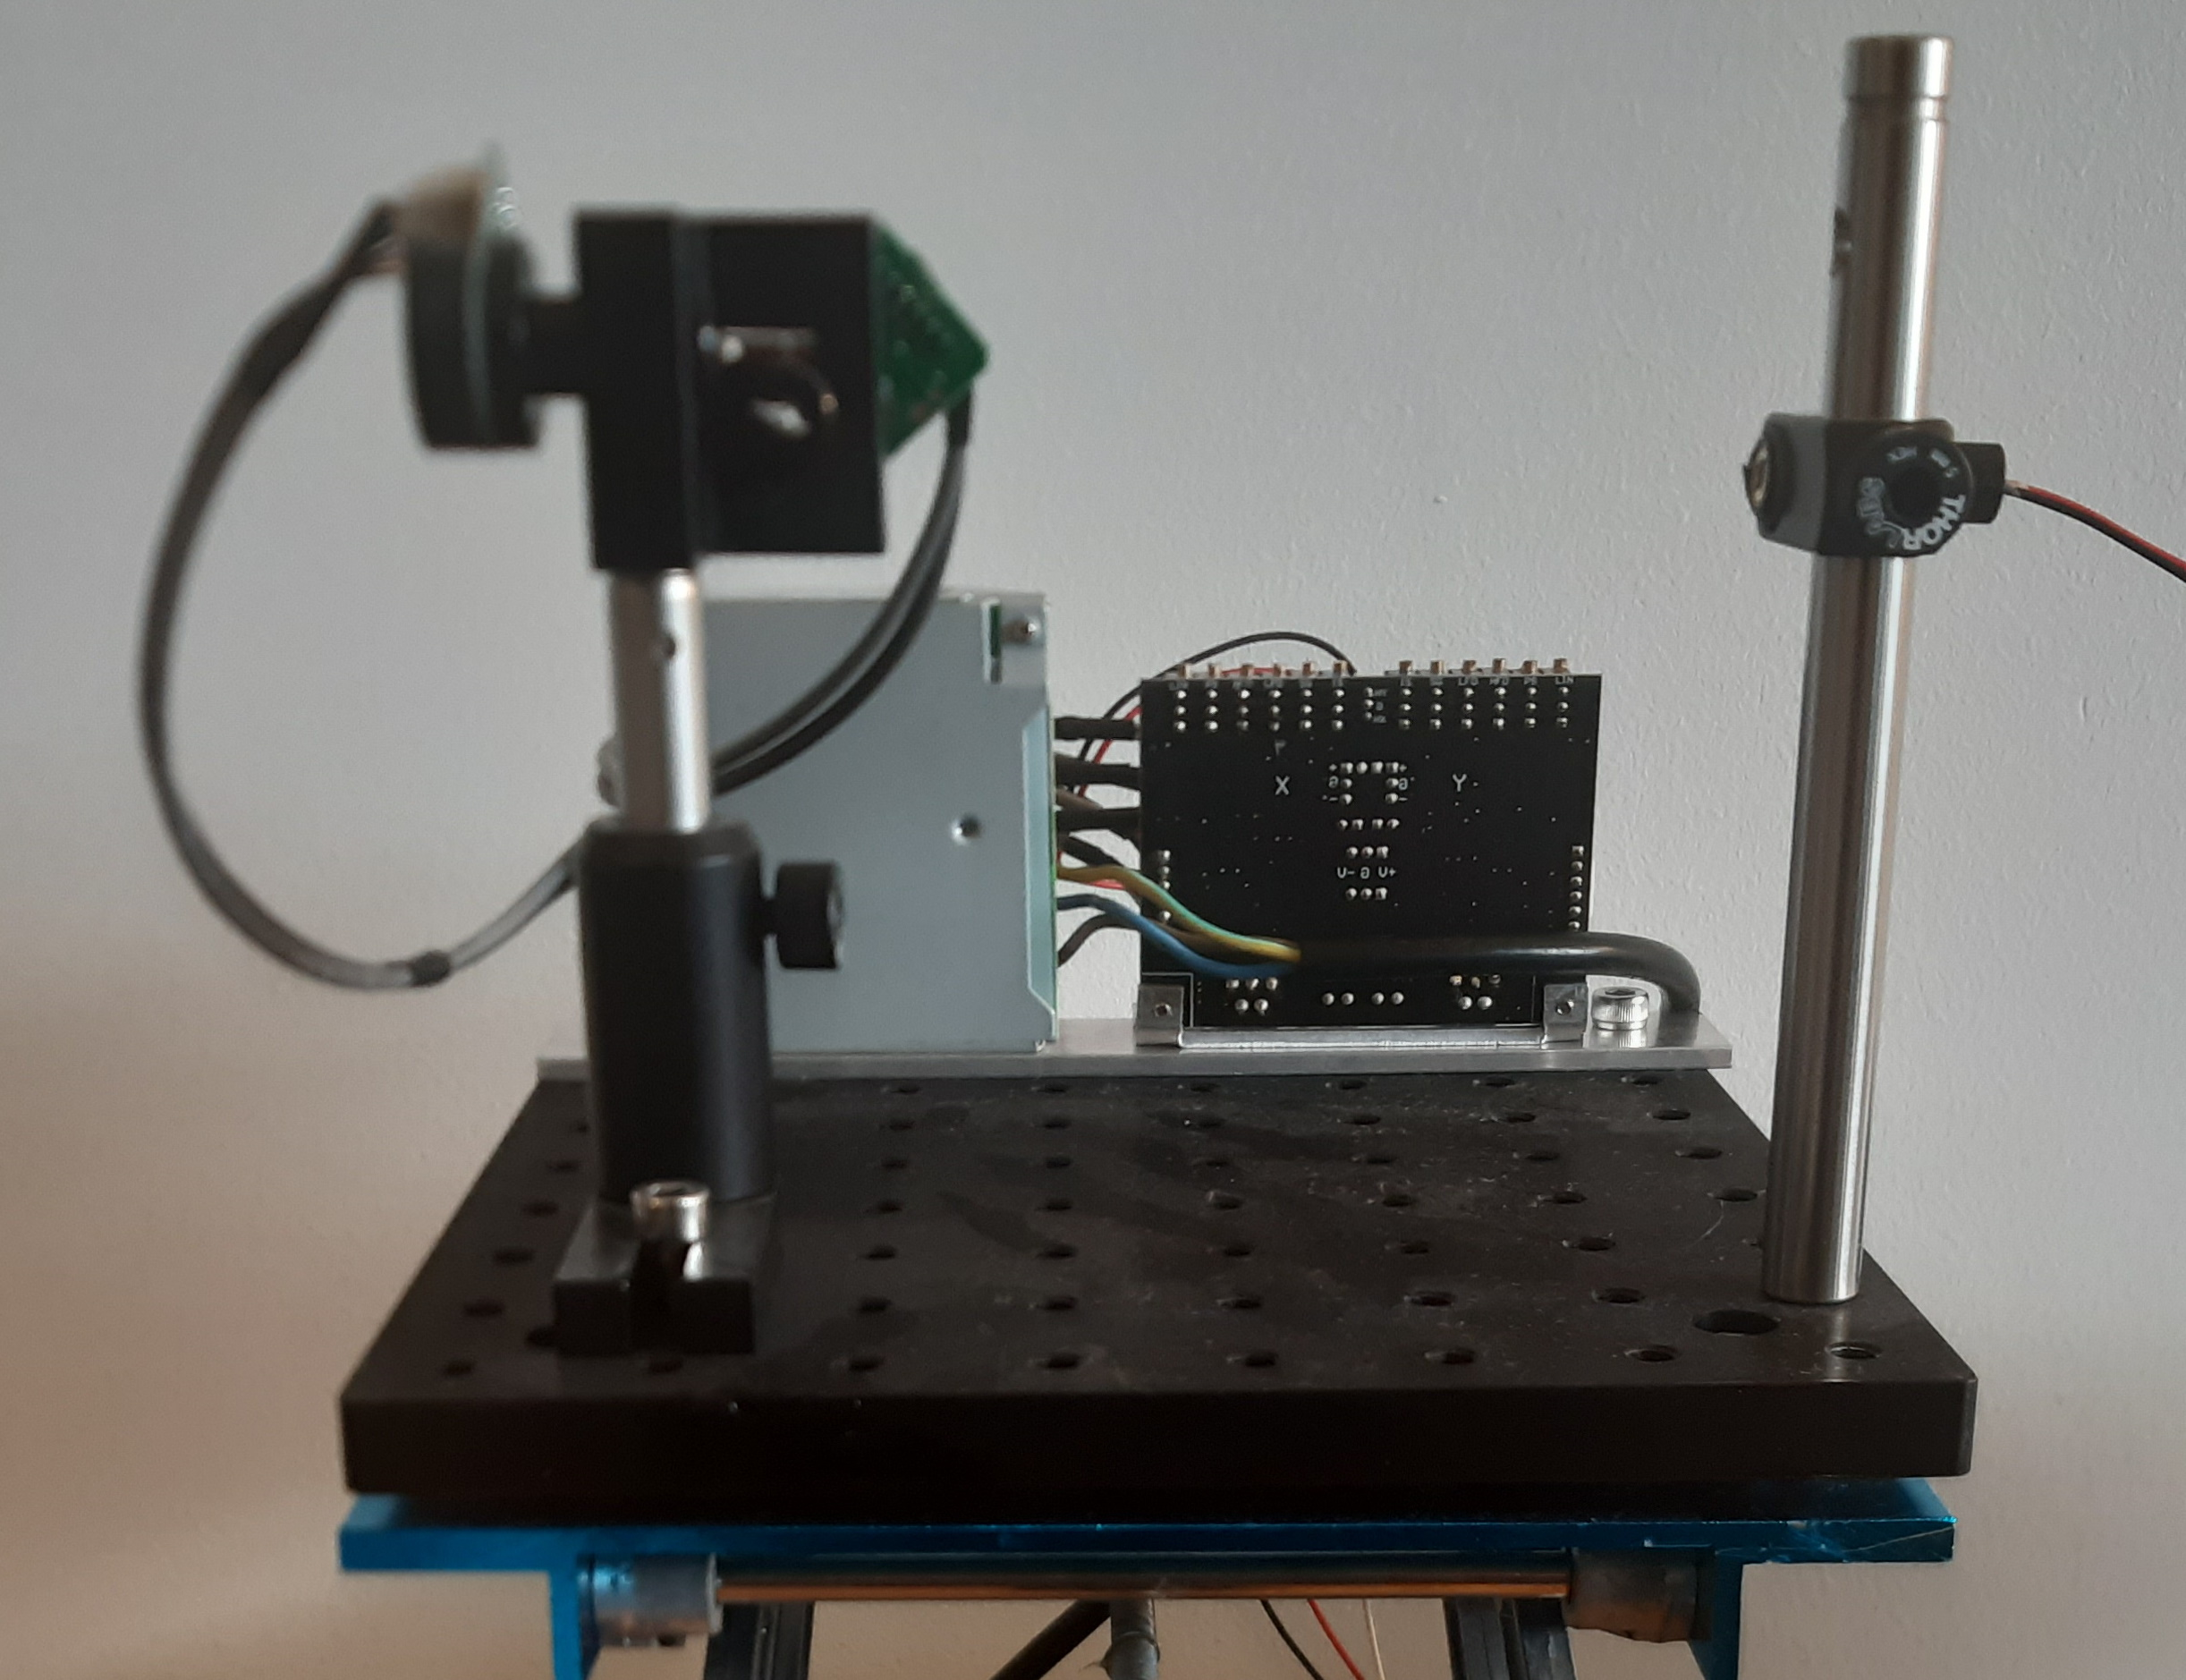
\includegraphics[width=\bildwidth]{pics/DutFront01.jpg}	\caption{DutFront01}	\label{DutFront01}	\end{figure}
% \begin{figure}[h!]	\centering	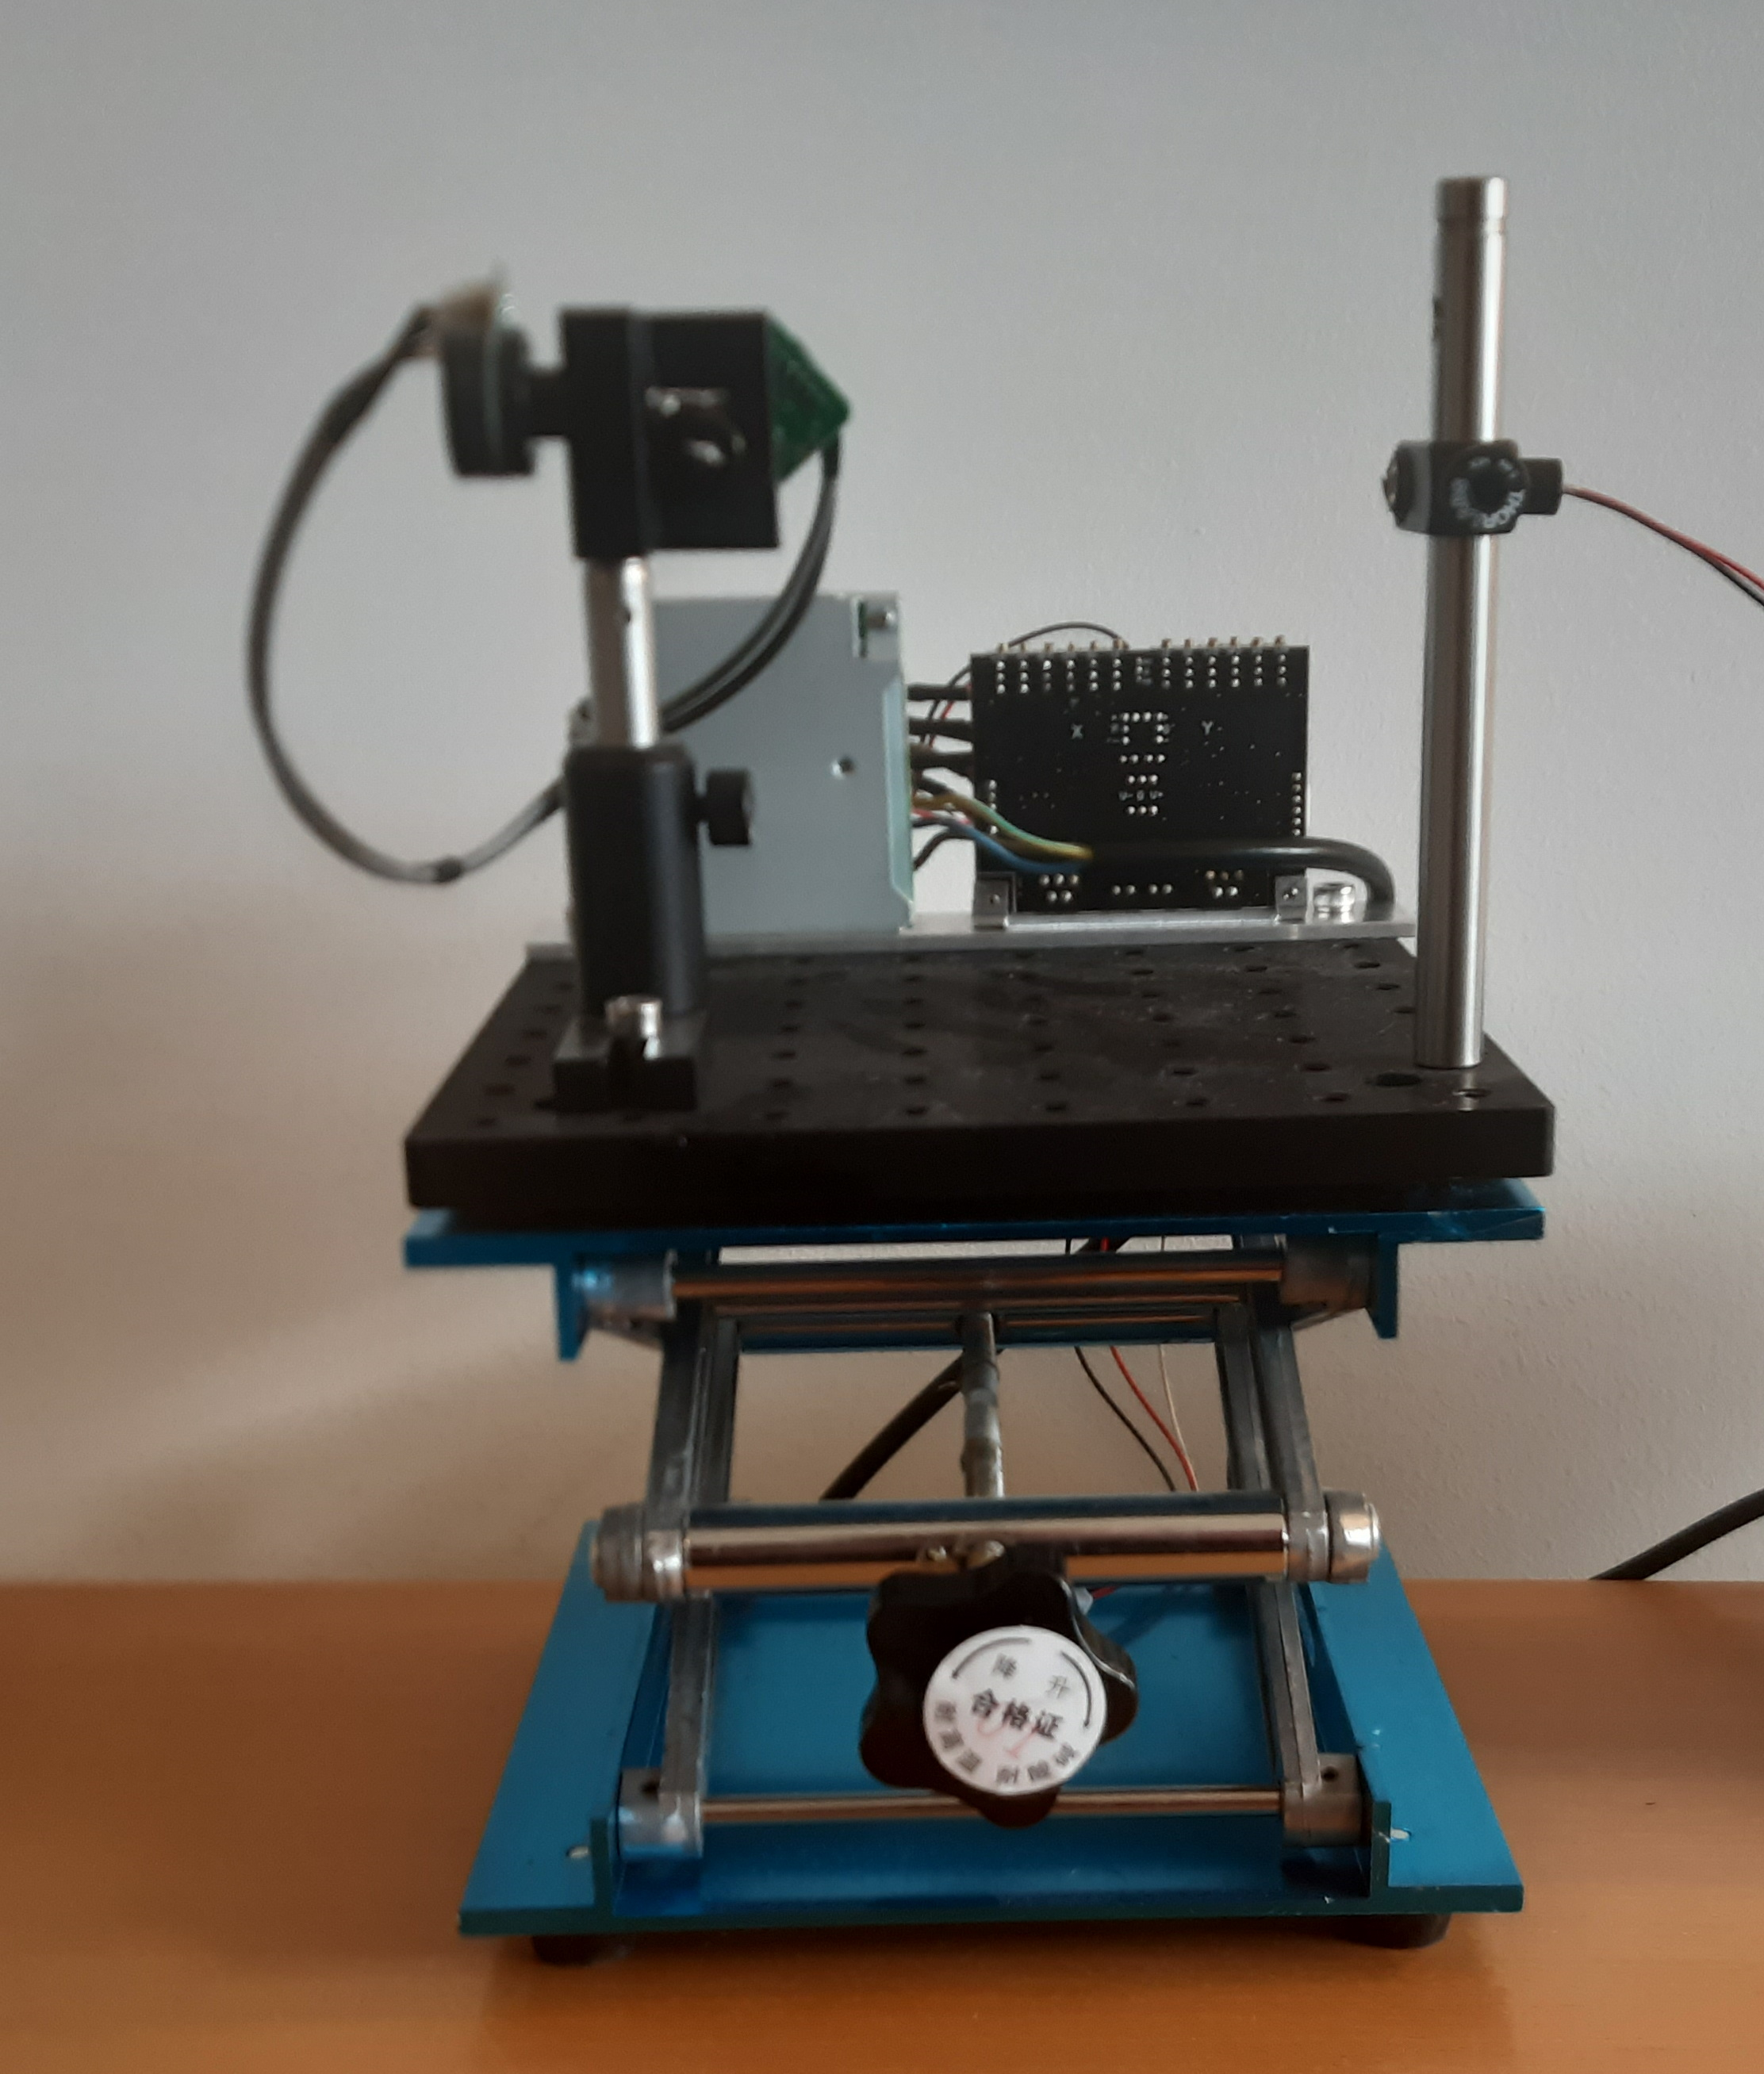
\includegraphics[width=\bildwidth]{pics/DutFront02.jpg}	\caption{DutFront02}	\label{DutFront02}	\end{figure}
% \begin{figure}[h!]	\centering	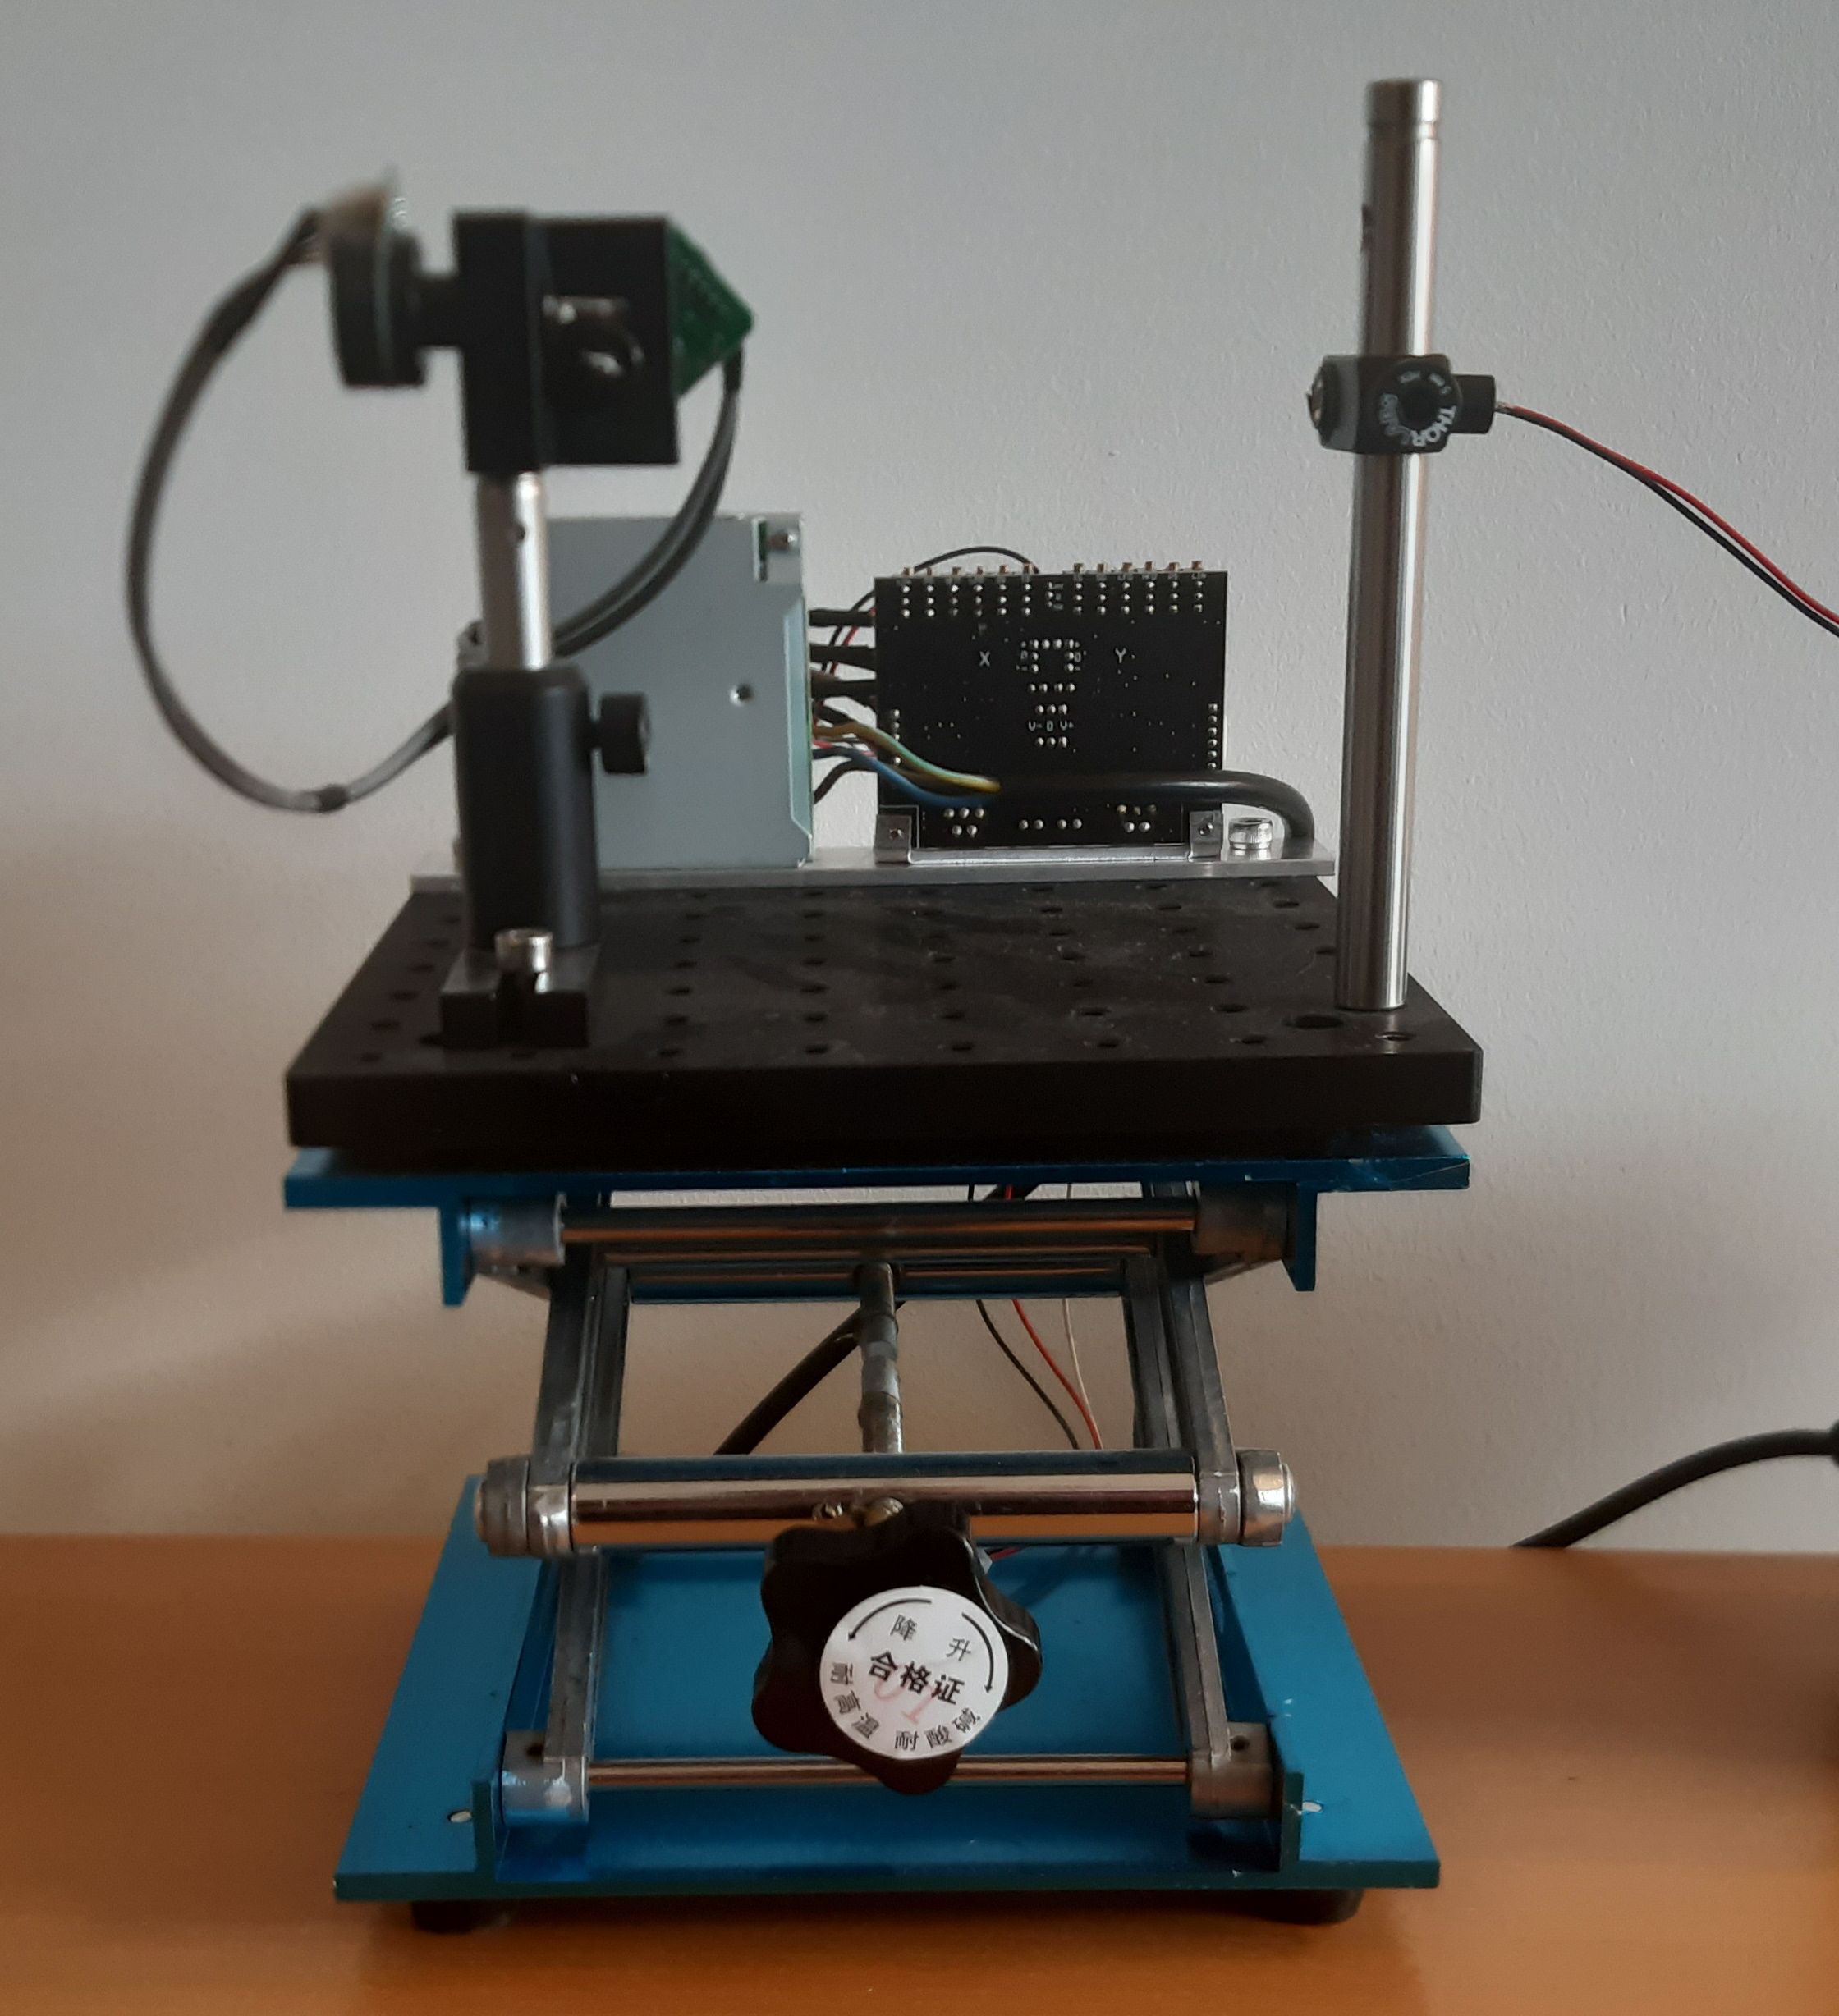
\includegraphics[width=\bildwidth]{pics/DutFront03.jpg}	\caption{DutFront03}	\label{DutFront03}	\end{figure}
% \begin{figure}[h!]	\centering	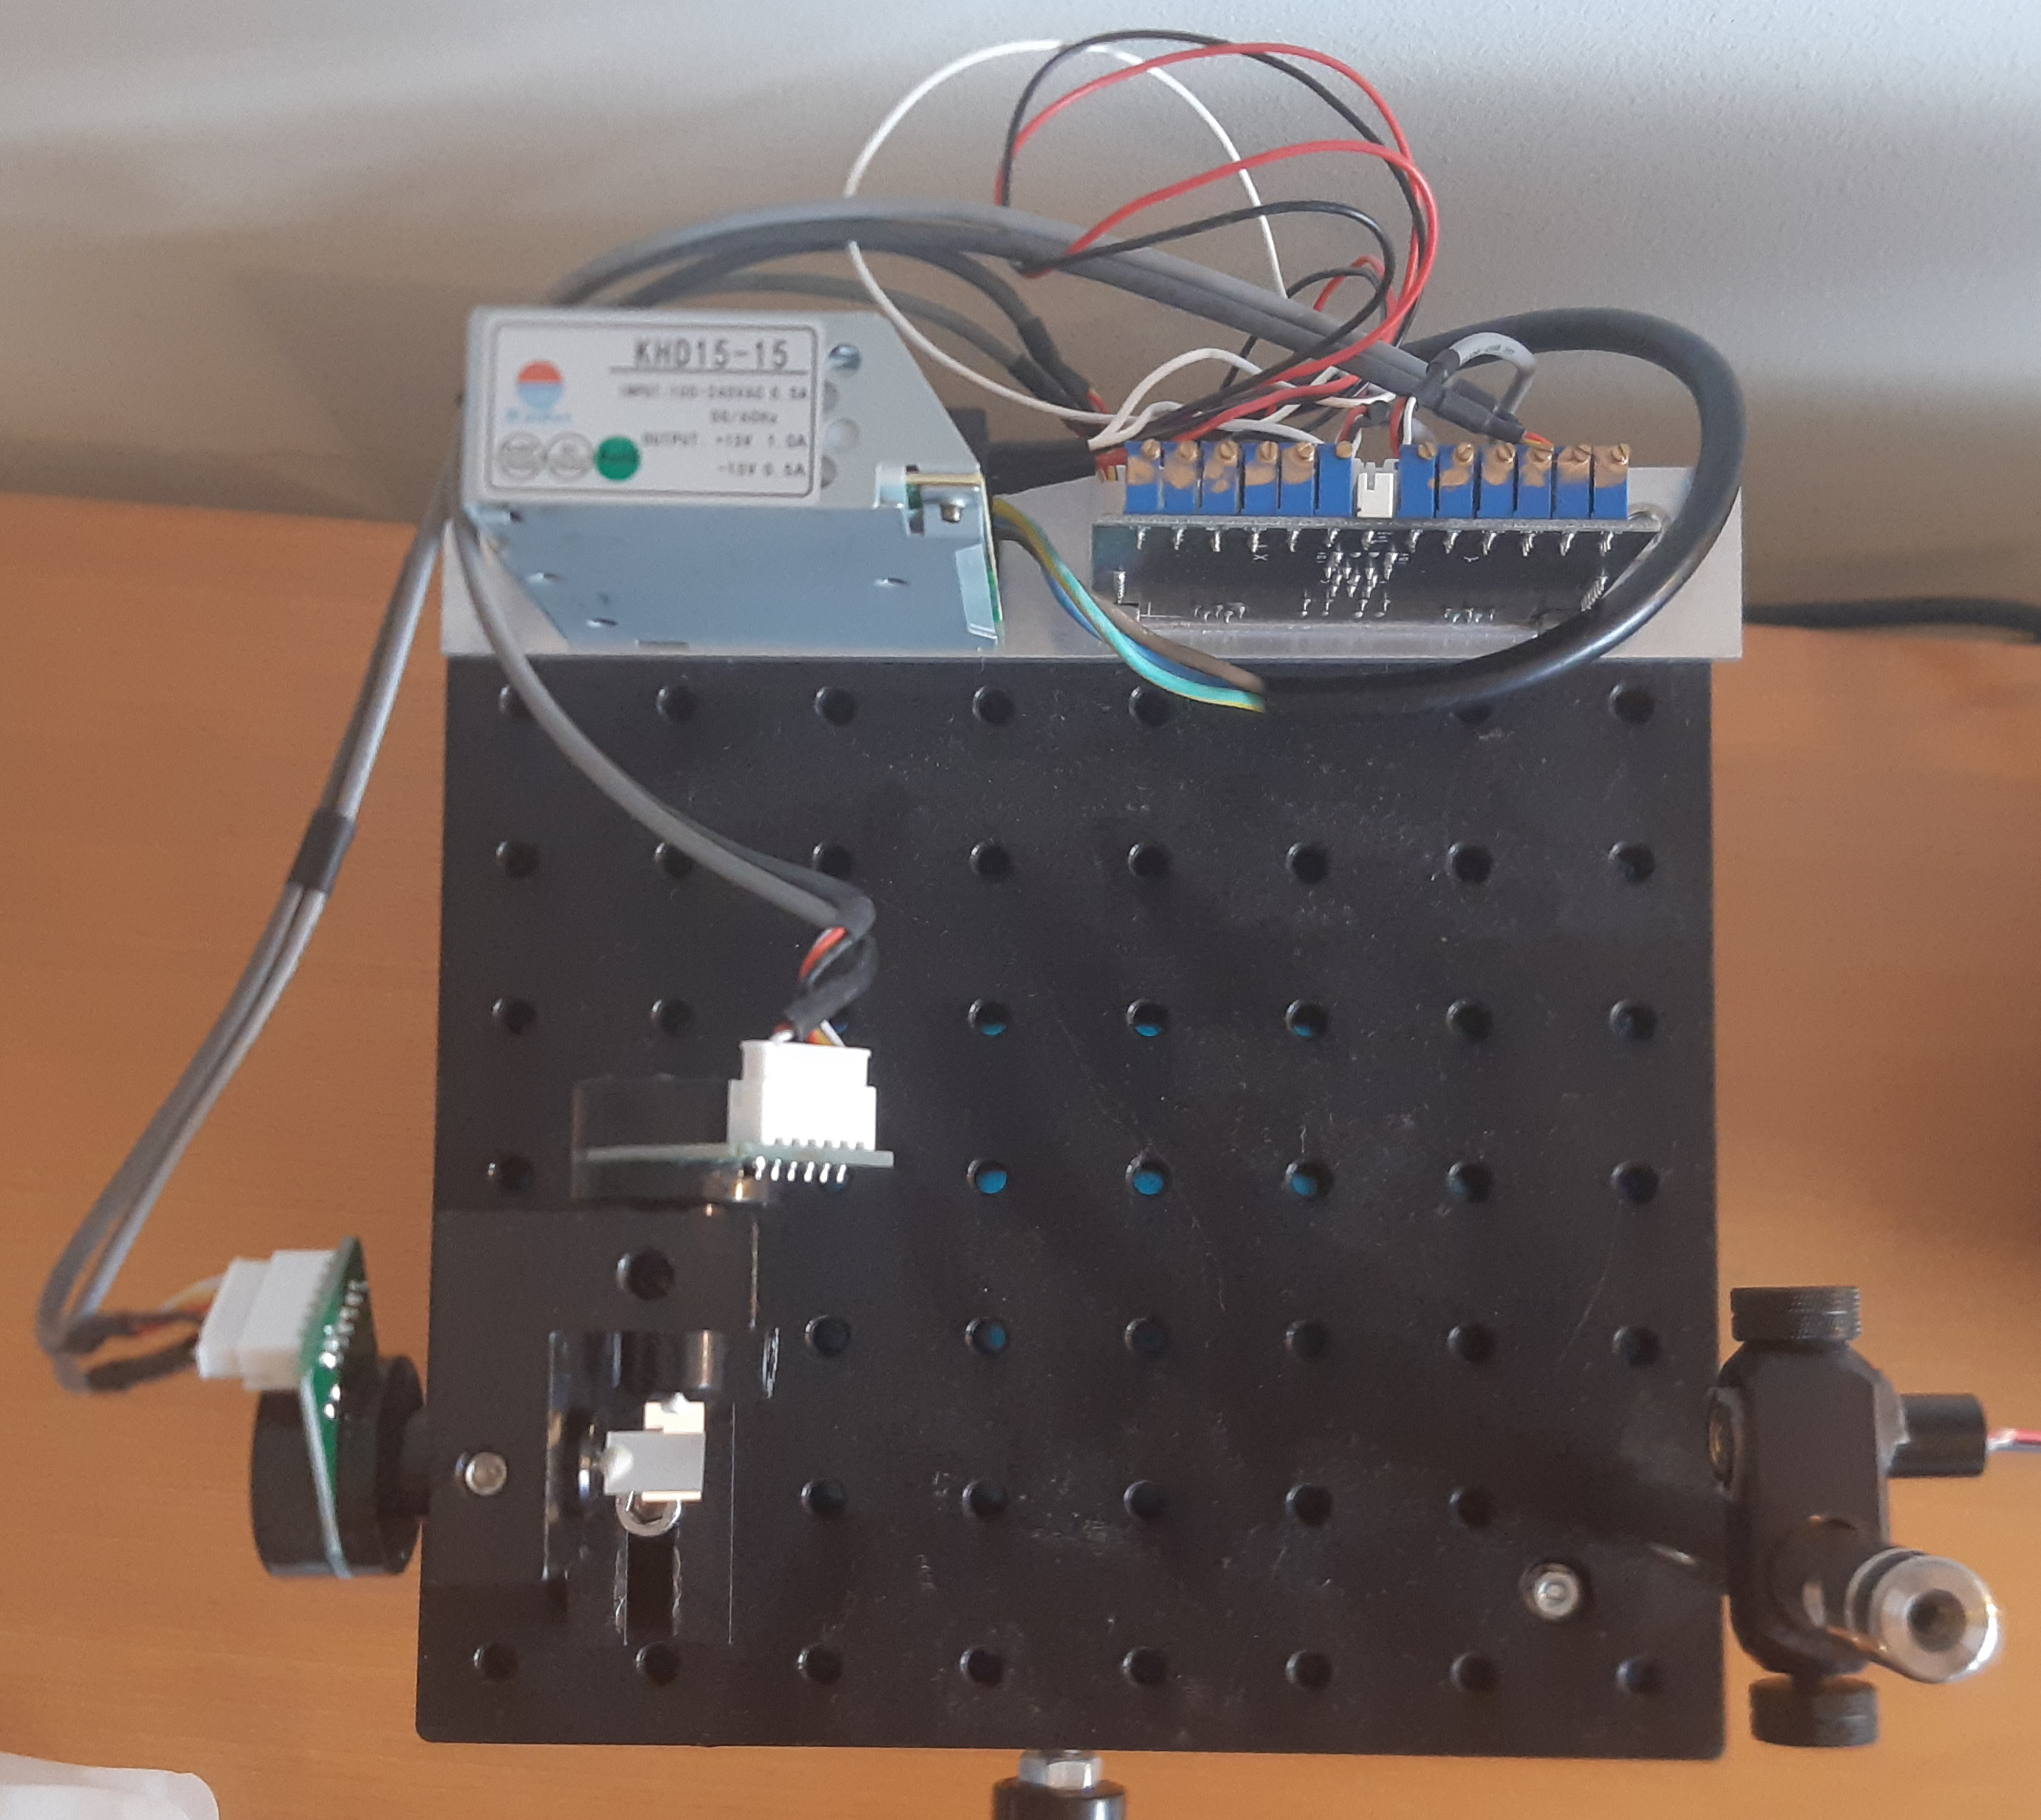
\includegraphics[width=\bildwidth]{pics/DutTop01.jpg}	\caption{DutTop01}	\label{DutTop01}	\end{figure}
\begin{figure}[h!]	\centering	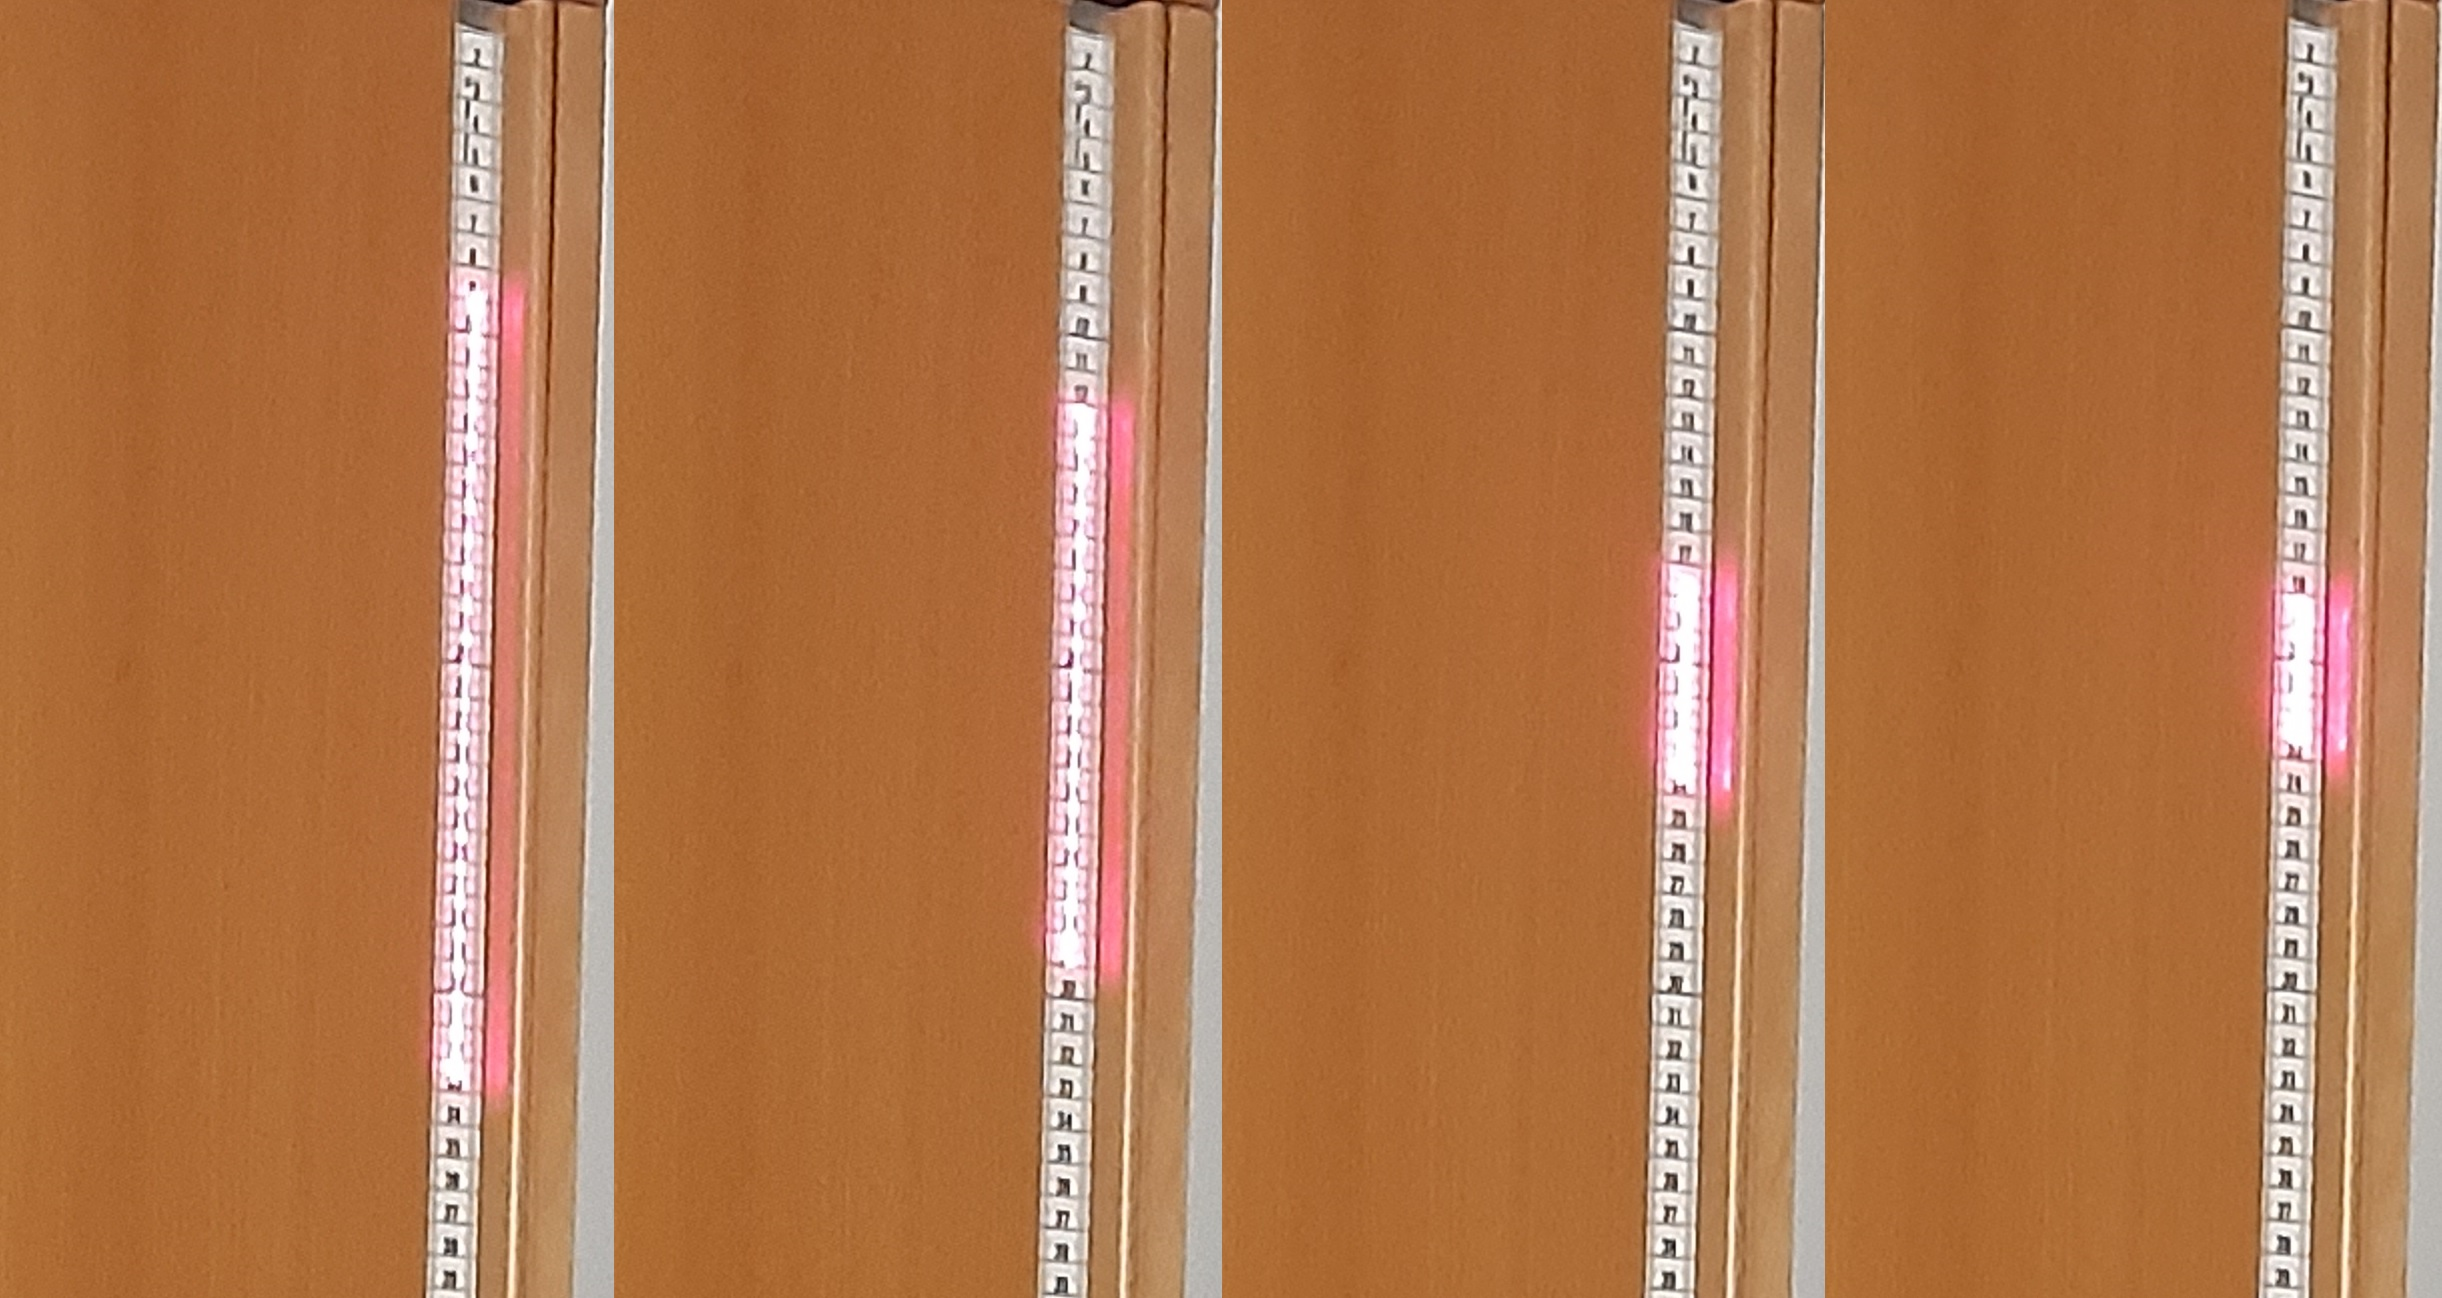
\includegraphics[width=\bildwidth]{pics/ImageMeasure01.jpg}	\caption{Abbilder von vier Messungen}	\label{ImageMeasure01}	\end{figure}
\bild{h!}{DetektorsForPhase}{Detektor zur Phasenmessung}{DetektorsForPhase}
% \begin{figure}[h!]	\centering	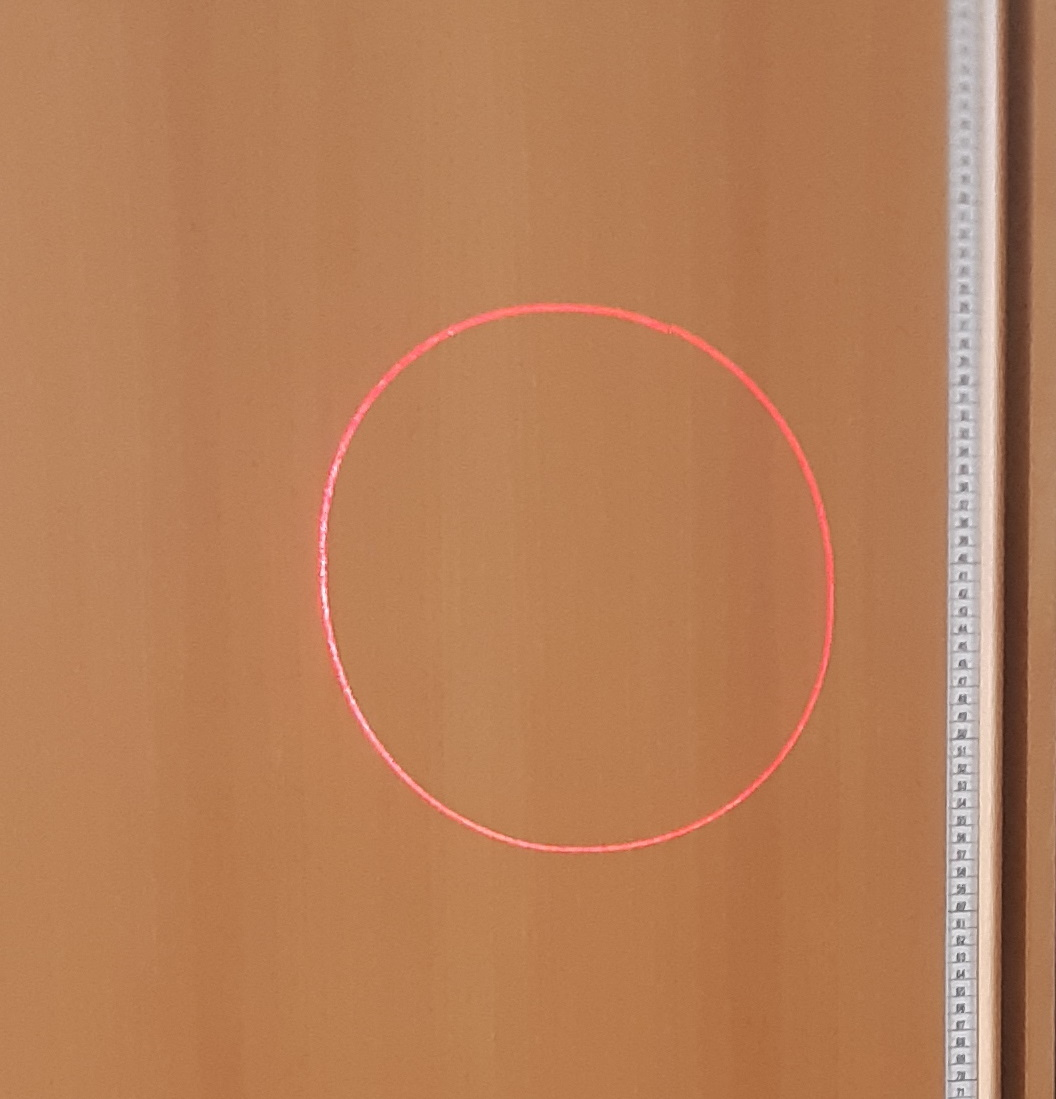
\includegraphics[width=\bildwidth]{pics/ImageXY01.jpg}	\caption{ImageXY01}	\label{ImageXY01}	\end{figure}
% \begin{figure}[h!]	\centering	\includegraphics[width=\bildwidth]{pics/.jpg}	\caption{}	\label{fig_sim}	\end{figure}

% \subsection{Messungen}
	% \begin{table}[h!]
	% \begin{center}
	% \begin{tabular}{l|l}
	% \input{Mess1.csv}
	% \end{tabular}
	% \caption{Messungcsv}
	% \label{Messungcsv}
	% \end{center}
	% \end{table}

\section{Ergebnisse}
\bild{h!}{Mess1log.eps}{Bode-Diagramm des \galvo }{Mess1log}
Die Ergebnisse der Messung sind in Abb.~\ref{Mess1log} dargestellt: Es existiert ein linearer Bereich unterhalb von 1kHz, bei dem die Auslenkung sehr exakt dem Steuersignal folgt. Oberhalb davon nimmt die Auslenkung mit steigender Frequenz ab und erreicht beim orangen Marker die -3dB-Grenzfrequenz mit 1.3kHz. Zwischen dem gruenen und roten Marker verdoppelt sich die Frequenz, was einer Oktave entspricht. Die Amplitude der Auslenkung faellt dabei um 6.43dB. Diese naeherungsweise 6dB/Oktave entsprechen 40dB/Dekade und somit einem System zweiter Ordnung der Form\cite{Staudecker}
	\begin{align*}
	% G(s) & = \frac{V}{(T_N s)^2 + 2 \xi T_N s +1} & \textrm{wird mit} \\
	% |s| & = |\alpha + j\omega| \overset{\alpha = 0} = \omega & \textrm{und} \\
	% T_N & = \frac{1}{\omega_0}  & 	\textrm{zu} \\
	G(\omega) & = \frac{V}{(\frac{\omega}{\omega_0} )^2 + 2 \xi \frac{\omega}{\omega_0}  +1} & \textrm{mit} \\
	% d &= 3190 mm \\
	\xi & = 1 \\
	\omega_0 &= 2\pi f_g \\
	f_{g}	& = 1300 Hz \\
	V &= 116.4 \frac{mm}{V} \\ % =  291mm/2.5V
	% dmax = 291mm
	% Vpp = 2.5V
	% f_{g,1Vpp} & = 1000 Hz \\
	\end{align*}
Die Daempfung $\xi$ mit '1' laesst sich aus dem Kurvenverlauf abschaetzen, da dieser keine Resonanzspitze an der Grenzfrequenz aufweist. Die Verstaerkung 'V' setzt die maximale Auslenkung mit der Amplitude der Steuerspannung ins Verhaeltnis. Auf eine Rueckrechnung von der Auslenkung auf den Drehwinkel des \galvo s wurde verzichtet. Fuer die Applikation ist die erreichbare Auslenkung in mm von Bedeutung, der Winkel stellt somit keine relevante Information dar. Beide vorhandenen  Galvanometer-Spiegel des Testobjektes wurden unter gleichen Bedingungen vermessen und zeigten nahezu identes Verhalten bezueglich ihrer Dynamik. Das Phasendiagramm ergibt sich mit der Formel \textrm{$\phi = 360^\circ f  \Delta t$} aus den gemessenen $\Delta t$. Diese wiederum stellen die Verzoegerung zwischen dem Nulldurchgang des Steuersignals, sowie der steigenden Flanke eines Opto-Detektors dar, der an der optischen Null-Position platziert ist. Der resultierende Verlauf entspricht einigermassen dem erwarteten Phasengang eines Systems 2ter Ordnung. Allerdings weist er schon bei tiefen Frequenzen eine Abweichung von der 0grad-Achse ab, was eine Totzeit des verwendeten Detektors vermuten laesst.
\section{Konklusion}
Das gewonnene Modell wird in einer Masterarbeit zur Adaptierung von Steuersignalen herangezogen. Das zugrundeliegende Konzept dazu nennt sich 'flachheitsbasierte Steuerung'. Hierbei wird das Steuersignal, unter Einbeziehung der Modell-Eigenschaften, so berechnet, dass der Ausgang einer Sollkurve folgt. Abgesehen von diesem direkten Nutzen der Messungen, verbessert sich auch das intuitive Verstaendnis der analysierten Komponenten und nuetzt damit bei der Applikation und Abschaetzung der Applizierbarkeit in OCT-Systeme. \\
Weitere Messungen mit unterschiedlichen Steuerspannungen und an mehreren Frequenzen, 	speziell im Bereich der Grenzfrequenz, sollen das bestehende Modell noch verfeinern. Auch soll die vermutete Totzeit des Opto-Detektors untersucht werden, damit praezisere Phasen-Messungen moeglich sind.

% \hfill rechtsbuendiger Text
\section*{Danksagung}
% \begin{itemize}
Martin Staudecker, Guenther Hannesschlaeger, Rankl Christian, Josef Langer und Silke Dorner, fuer die Assistenz bei Messungen.
% \end{itemize}
\label{cha:galvoChar}

% \chapter{Closing Remarks}
\label{cha:Closing}

%%%-----------------------------------------------------------------------------
\appendix                                                             % Appendix 
%%%-----------------------------------------------------------------------------

% \chapter{Technical Details}
\label{app:TechnicalDetails}



 % Technical supplements
\chapter{Supplementary Materials}
\label{app:materials}


List of supplementary data submitted to the degree-granting institution for archival storage
(in ZIP format).

% Use this as an example only, adapt the structure to your requirements!

\section{PDF Files}
\begin{FileList}{/}
\fitem{thesis.pdf} Master/Bachelor thesis (complete document)
\end{FileList}

\section{Media Files}
\begin{FileList}{/media}
\fitem{*.ai, *.pdf} Adobe Illustrator files
\fitem{*.jpg, *.png} raster images
\fitem{*.mp3} audio files
\fitem{*.mp4} video files
\end{FileList}


% \section{Online Sources (PDF Captures)}
% \begin{FileList}{/online-sources}
% \fitem{Reliquienschrein-Wikipedia.pdf} \parencite{WikiReliquienschrein2020}
% \end{FileList}




 % Contents of the CD-ROM/DVD
% \chapter{Questionnaire}
\label{app:Questionnaire}





 % Chronological list of changes
% \chapter{\latex Source Code}
\label{app:SourceCode}

 % Source text of this document

%%%-----------------------------------------------------------------------------
\backmatter                           % Back part (bibliography, glossary, etc.)
%%%-----------------------------------------------------------------------------

	\section{Abbreviations and Acronyms}
	\begin{table}[h!]
			\begin{tabular}{|p{2cm}|l|}
			\hline	
			uC		& MicroController							\\ \hline
			FW		& Firmware, the Software, running on the uC \\ \hline	
			OCT		& Optical Coherence Tomography				\\ \hline	
			SW		& Software, the Software, running on the OCT-System 	\\ \hline	
			FSM 	& Finite State Machine									\\ \hline
			CRC		& Cyclic Redundancy Check								\\ \hline
			IO		& Input-Output, bidirectional Communcation Lines 		\\ \hline
			USB		& Universal Serial Bus									\\ \hline
			VCP		& Virtual Com Port, a serial connection via USB			\\ \hline
			% CDC		& communications device class, implements VCP over USB	\\ \hline
			USB		& Universal Serial Bus									\\ \hline
			SCPI	& Standard Commands for Programmable Instruments, as defined by IEEE 488.2	\\ \hline
			% r.SCPI	& RECENDTs adaption of SCPI, employed for Communication between SW and FW	\\ \hline
			LUT		& Look-up-table											\\ \hline
			IRQ		& Interrupt request										\\ \hline
			ISR		& Interrupt-service-routine, a function within the FW, that is called by an IRQ	\\ \hline
			HW		& Hardware, the entirety of uC, the PCB and peripherals	\\ \hline
			SLD		& Super luminiscence Diode								\\ \hline
			AIM		& Aiming Laser											\\ \hline
			CAM		& Camera												\\ \hline
			LED		& Light emitting diode									\\ \hline
			LSB		& Least significant bit									\\ \hline
					% & \\ \hline
					% & \\ \hline
			\end{tabular}
			\caption{Abbreviations}
		\end{table}


\MakeBibliography % References

%%%-----------------------------------------------------------------------------
% Special page for checking print size
%%%-----------------------------------------------------------------------------

% \chapter*{Check Final Print Size}

\begin{center}
{\Large --- Check final print size! ---}

\bigskip

\calibrationbox{100}{50} % width/height of box in mm

\bigskip

{\Large --- Remove this page after printing! ---}

\end{center}



%%%-----------------------------------------------------------------------------
\end{document}
%%%-----------------------------------------------------------------------------
